\documentclass[12pt]{article}
\usepackage{geometry}
\usepackage[utf8]{inputenc}
\usepackage[T1]{fontenc}
\usepackage{latexsym,amsmath,amssymb,amsfonts}
\usepackage[spanish]{babel} 
\usepackage{time}
\usepackage{setspace}          % Para manejar el espacio interlineal
\usepackage{fancyhdr}          % Para personalizar encabezados y pies de página
\usepackage{graphicx}
\usepackage{amsmath}
\usepackage{relsize}
\hyphenation{Mod-NVD}
\usepackage{float}
\usepackage{placeins}
\usepackage[autostyle]{csquotes}
\usepackage[backend=biber,style=apa,sorting=nyt]{biblatex}
\addbibresource{referencias/Referencias.bib}
\spanishdecimal{.}
\usepackage{makecell} % para permitir saltos de línea en una celda

\usepackage{cellspace} % Para agregar padding vertical a las celdas

% Configuración de padding
\setlength{\tabcolsep}{5pt} % Padding horizontal
\setlength\cellspacetoplimit{10pt} % Padding vertical superior
\setlength\cellspacebottomlimit{10pt} % Padding vertical inferior

% Configuración de la sangría
\setlength{\parindent}{2ex}   % Sangría de 5 espacios (aproximadamente 5ex)

% Configuración del espacio interlineal
\onehalfspacing
\usepackage{enumitem} % Paquete para personalizar listas
 
\usepackage{array} % Para personalizar el estilo de las celdas
 
 % Configuración de padding
 \renewcommand{\arraystretch}{1.6} % Padding vertical (1.5 es el factor de espaciado)       
        

\geometry{
	paperwidth=21.59cm,
	paperheight=27.94cm,
	left=4.0cm,
	right=1.5cm,
	top=3cm,
	bottom=3cm,
}

\parindent = 0mm
 
\begin{document}
	
	\thispagestyle{empty}
	\hskip-2.15cm
	\begin{minipage}[c][1\totalheight][s]{3.5cm} 
		\begin{center}
			
\includegraphics[height=2.5cm]{img/uady.png}\\[10pt]
		\end{center}
	\end{minipage}\begin{minipage}[c][1\totalheight][s]{12cm} 
		\begin{center}
			{\fontfamily{phv}\selectfont\Large\textbf {UNIVERSIDAD AUTÓNOMA DE YUCATÁN}}
			\vspace{0.3cm}
			\hrule height1.5pt
			\vspace{.3cm}
			{{\fontfamily{phv}\selectfont FACULTAD DE MATEMÁTICAS\\UNIDAD MULTIDISCIPLINARIA TIZIMÍN}}
		\end{center}
	\end{minipage}\begin{minipage}[c][1\totalheight][s]{3cm} 
		\begin{center}
			
\includegraphics[height=2.5cm]{img/matem.png}\\[10pt]
		\end{center}
	\end{minipage}\quad
	\vspace{.01cm}
	
	\hskip -0.9cm
	\begin{minipage}[c][1\totalheight][s]{1cm}
		\begin{center}
			\hskip2pt\vrule width3.5pt height19.5cm\hskip1mm
			\vrule width0.5pt height19.5cm\\[10pt]
		\end{center}
	\end{minipage}\hspace{0.5cm}\begin{minipage}[c][1\totalheight][s]{14cm}
		\begin{center}
			\vspace{1.5cm}
			
			{\fontfamily{phv}\selectfont\Large\textbf{Una propuesta basada en estimadores Bootstrap robustos para la evaluación de la precisión de un modelo con la técnica de regresión lineal}}
			
			\vspace{1cm}
			{{\fontfamily{phv}\selectfont\large Tesis presentada por el:}}\\
			
			\vspace{0.5cm}
			
			{{\fontfamily{phv}\selectfont\large Br. Irving Geyler Cupul Uc}}\\
			
			\vspace{1.5cm}
			
			{\fontfamily{phv}\selectfont\large En su examen profesional en opción al título de:}
			
			\vspace{0.5cm}
			
			{\fontfamily{phv}\selectfont\large Licenciado en Ingeniería de Sofware}
			
			\vspace{1.2cm}
			
			{\fontfamily{phv}\selectfont\large Asesores:}
			
			\vspace{0.5cm}
			
			{\fontfamily{phv}\selectfont\large M.C. Luis Colorado Martínez\\M.C. Salvador Medina Peralta}
			
			\vspace{4cm}
			{{\fontfamily{phv}\selectfont Tizimín, Yucatán, Diciembre 2024}}
		\end{center}
	\end{minipage}
	\newpage
	
	\input{2_agradecimientos-dedicacion.tex}
	\section*{Resumen}

En este trabajo se propone un método que permite evaluar la precisión de un modelo con la técnica de regresión lineal; y se basa en implementar diversos esquemas de remuestreos y estimar la precisión, a través de intervalos de confianza Bootstrap para el coeficiente de determinación $R^2$, del modelo de regresión entre los valores reales y predichos del modelo que se desea evaluar.\\

Tomando en cuenta el cumplimiento o no de los supuestos de normalidad y varianza constante, se consideraron cuatro escenarios posibles (NVC, NNVC, NVD y NNVD), como resultados de la combinación de ambos supuestos; y para estimar la distribución del coeficiente de determinación $R^2$, se implementaron ocho esquemas de remuestreos: el Bootstrap simple; el Wild Bootstrap robusto propuesto en \textcite{rana-2012}, ejecutado con los tres esquemas propuestos por \textcite{wu-1986} y con los dos esquemas propuestos por \textcite{liu-1988}; el Bootstrap de residuales balanceado y el Bootstrap pareado balanceado. Se proponen los intervalos percentiles y el Bca para estimar $R^2$ y para su cómputo se utilizan $B=1,000$ remuestras para cada uno de los esquemas Bootstrap.\\ 

Se realizó un estudio de simulación para comparar las eficiencias de los intervalos de confianza para cada tipo de supuesto con respecto a los diferentes esquemas Bootstrap, tamaños de muestra y tipo de modelo; para ello se simularon y evaluaron $60,000$ modelos Exactos-Precisos (EP) y $60,000$ modelos Exactos-Imprecisos (EI); para cada modelo se identificó la $R^2$ de origen utilizada para su simulación. Se simularon modelos de tamaños $n=10, 15, 20, 25, 30, 35$ para cada uno de los supuestos y tipo de modelo.\\

Se consideraron tres criterios principales para determinar las eficiencias de los intervalos para cada esquema Bootstrap, el primer criterio determina la eficiencia como el porcentaje de las veces en que el intervalo contiene a la $R^2$ de origen para los modelos EP simulados; y viceversa, para los modelos EI la eficiencia se determinó como el porcentaje de las veces en que el intervalo de confianza no contiene a la $R^2$ de origen. El segundo criterio determina la eficiencia como el porcentaje de las veces en que ambos intervalos contienen de manera simultánea a la $R^2$ de origen para los modelos EP y de manera viceversa cuando ambos no la contienen para los modelos EI; y el tercer criterio determina la eficiencia como el porcentaje de las veces en que uno de los intervalos es más estrecho que el otro cuando ambos intervalos contienen simultáneamente la $R^2$ de origen para los modelos EP y de manera viceversa uno de los intervalos es más estrecho que el otro cuando ambos no la contienen simultáneamente para los modelos EI.\\

Se analizaron los resultados del estudio de simulación a través de un ANOVA factorial y se determinó con al menos un 95\% que para los supuestos NVC, NNVC o NVD se utilice el ICB Percentil con el esquema de remuestreo Liu2 sin importar el tamaño de muestra. Y se determinó con al menos el 88.8\% que para el supuesto NNVD se utilice el ICB BCa con el esquema de remuestreo pareado balanceado; con la limitación de que para modelos EI con tamaños de muestra “pequeño” $n=10, 15, 20,$ no se obtuvo un buen desempeño. \\


Con el propósito de que los resultados de este trabajo conformen una herramienta que permita evaluar la precisión de un modelo, se consideró como propuesta final: para los supuestos NVC, NNVC o NVD se utilice el ICB Percentil con el esquema de remuestreo Liu2 (NVC: residuales de regresión lineal simple, NNVC: residuales robustos sin ponderar y NVD: residuales robustos ponderados) y para el supuesto NNVD se utilice el ICB BCa con el esquema de remuestreo Pareado Balanceado. La propuesta final se implementó en el lenguaje R \parencite{R-2024}; y se ilustra con la evaluación de dos modelos que se ajustan a los diferentes escenarios contemplados en la propuesta y que corresponden a casos reales. Para la ganancia diaria de peso en ovinos, el modelo resultó ser de tipo NVC y preciso, coincidiendo con \textcite{balam-2012}, cabe señalar que usó ICB BCa con residuales balanceados y en este trabajo se usó ICB Percentil con el esquema de remuestreo Liu2. Para el volumen por parcela, el modelo resultó de tipo NNVD y preciso, coincidiendo con \textcite{balam-2012}, tanto en la decisión como en el esquema e ICB que utilizó.
	\newpage
	\tableofcontents
	\newpage
	\listoffigures
	\newpage
	\section{Introducción}
Los modelos son representaciones matemáticas de mecanismos que rigen fenómenos naturales que no se reconocen, controlan o comprenden plenamente, y el proceso de modelación abarca varios pasos que comienzan con una declaración clara de los objetivos del modelo, supuestos sobre sus límites del modelo, la adecuación de los datos disponibles, el diseño de la estructura del modelo, la evaluación de las simulaciones y la aportación de la información para los procesos de recomendación y rediseño (Tedeschi, 2006).
\vspace{.5cm}
 
La validación de un modelo en predicción del sistema es la comparación por medio de algún método de las predicciones del modelo con los valores observados del sistema real para determinar su capacidad predictiva; en esta etapa del proceso de modelación matemática se evalúan la exactitud y precisión del modelo, la primera se refiere a la proximidad de las predicciones $( z )$ con los valores observados $( y )$, por ejemplo, sus diferencias $ ( d=y-z ) $ del cero y la segunda a la dispersión de los puntos $ (z, y) $; sin embargo, en presencia de exactitud la precisión se mide cuantificando la dispersión de dichos puntos respecto a una referencia, por ejemplo, la recta determinista $ y=x $, o bien, evaluar la varianza de las diferencias $ (\sigma_{D}^{2}) $ alrededor del cero $ (\mu_{D}=0) $ (Medina-Peralta et al., 2017).
\vspace{.5cm}
 
En la literatura se han expuesto diferentes enfoques y técnicas para validar modelos. Las técnicas de validación se pueden agrupar en cuatro categorías principales: evaluación subjetiva (involucra a un número de expertos en el campo de interés), técnicas visuales (gráficas comparativas), medidas de desviación (basadas en las diferencias entre valores observados y simulados) y pruebas de estadísticas (Mayer y Butler, 1993).
\vspace{.5cm}
 
Entre las técnicas inferenciales, una de las más utilizadas es la Regresión Lineal (RL) entre los observados del sistema real $ (y) $ en función de los predichos del modelo a evaluar $ (z) $, $ y_{i} = \beta_{0} + \beta_{1}z_{i} +\epsilon $  donde $ \epsilon_{i} \sim NI(0,\sigma^{2}) $ ; la exactitud se evalúa por medio de una $ F $ conjunta verificando si simultáneamente $ \beta_{0} $ y $ \beta_{1} $ son cero y uno respectivamente (Yang et al., 2004; Tedeschi, 2006; Montgomery et al., 2012); y la precisión se evalúa por medio del coeficiente de determinación $ R^{2} $ (Balam, 2012), mientras más cerca esté de uno el modelo es más preciso.
Adicionalmente, Zacarias (2023) desarrolló un método no paramétrico para evaluar la exactitud de un modelo con la técnica de regresión lineal cuando no se cumplen los supuestos de normalidad y/o varianza constante, basada en la construcción de una región de confianza Bootstrap para el vector de parámetros de regresión. De modo que si el vector  $ (\beta_{0},\beta_{1})=(0,1) $ está contenido en dicha región de confianza, se concluye el modelo es exacto en predicción del sistema. En Zacarias (2023), para garantizar que las estimaciones sean confiables y resistentes a las influencias de datos atípicos se utilizaron estimadores de regresión robustos y se implementó el Wild Bootstrap robusto propuesto en Rana et al. (2012) bajo tres esquemas de remuestreo propuestos por (Wu, 1986) y dos propuestos por (Liu, 1988).
\vspace{.5cm}

Febles (2014) propuso un método para simular modelos que implica la creación de una muestra pareada de valores observados y predichos $ (z_{i},y_{i}) $ basada en la media $ (\bar{z}) $ y los parámetros $ (\beta_{0}, \beta_{1}, R^{2}, SCE) $ de un modelo de regresión entre los observados y predichos. Este método simula modelos de cuatro tipos (exacto-preciso, exacto-impreciso, inexacto-preciso, inexacto-impreciso) y considera cuatro casos de supuestos (normalidad-varianza constante, no normalidad-varianza constante, normalidad-varianza no constante, no normalidad-varianza no constante) en función de la normalidad y la varianza en el modelo de regresión. En Zacarías (2023), se mejoraron los simuladores de Febles (2014) al seleccionar valores plausibles de $ SCE $ que generan modelos exacto-precisos independientemente del supuesto cumplido. Además, se determinó una constante para el ancho de una banda horizontal donde se distribuyen los valores predichos y residuales. Se reemplazó el estadístico de Kolmogorov-Smirnov por el de Lilliefors para las pruebas de normalidad, y se implementó la prueba de Breusch-Pagan cuando los residuales cumplen el supuesto de normalidad y la de White cuando los residuales no se ajustan a la distribución normal.
\vspace{.5cm}

Balam (2012), para medir la precisión de un modelo con regresión lineal, propone la construcción de un intervalo de confianza Bootstrap de residuales balanceado con sesgo corregido acelerado BCa, para los casos cuando se cumple el supuesto de varianza constante, independiente si se cumple o no el supuesto de normalidad; y para los casos cuando no se cumple el supuesto de varianza constante, independientemente si se cumple o no el de normalidad, se construye un intervalo de confianza Bootstrap pareado balanceado método percentil con sesgo corregido acelerado BCa.
\vspace{.5cm}

Para medir la precisión se puede considerar el Wild Bootstrap robusto propuesto en Rana et al. (2012) ya que este considera la utilización de estimadores robustos y otros esquemas de remuestreo diferente al Bootstrap simple.
En el presente trabajo se implementará una propuesta a través de intervalos de confianza para evaluar la precisión de un modelo con la técnica de regresión lineal, basada en estimadores robustos y los esquemas de remuestreo Bootstrap propuestos por Rana et al. (2012) e implementados en Zacarías (2023). Se realizará un estudio de simulación para evaluar la eficacia de esta propuesta y se implementará en el lenguaje R (R Core Team, 2024).

	\newpage
	\section{Objetivos}
\subsection{Objetivo general}
Determinar la precisión de un modelo con la técnica de regresión lineal por medio de intervalos de confianza basado en diferentes esquemas de remuestreo Bootstrap y medir sus eficiencias a través de un estudio de simulación.
\vspace{.5cm}
\subsection{Objetivos específicos}
\begin{enumerate}
\item Desarrollar la metodología para medir la precisión de un modelo con la técnica de regresión lineal por medio de intervalos de confianza basado en diferentes esquemas de remuestreo Bootstrap.
\item Determinar la precisión de un modelo cuando se cumplan los supuestos de normalidad y varianza constante.
\item Determinar la precisión de un modelo cuando no se cumplan los supuestos de normalidad y/o varianza constante.
\item Diseñar e implementar un estudio de simulación para evaluar la eficiencia de la metodología propuesta.
\item Simular modelos exactos-precisos (EP) y modelos exactos-imprecisos (EI) mediante la propuesta de \textcite{febles-2014} y \textcite{zacarias-2023}; cuando se cumplan o no los supuestos de normalidad e igualdad de varianzas.
\item Determinar la eficiencia de los esquemas Bootstrap propuestos para medir la precisión de un modelo.
\end{enumerate}

	\newpage
	\section{Marco Teórico}

\subsection{Validación de Modelos}
Los modelos son representaciones matemáticas de los mecanismos que rigen los fenómenos naturales \parencite{tedeschi-2006} o como una construcción matemática diseñada para estudiar un sistema del mundo real o fenómeno (Giordano et al., 1997).\\

\textcite{medina-peralta-2017} indican que la validación de un modelo en la predicción del sistema implica la comparación, por medio de algún método, de las predicciones del modelo con los valores observados del sistema real para determinar su capacidad predictiva.\\

\textcite{mayer-butler-1993}, clasifican los métodos de validación de modelos en Evaluación Subjetiva, Técnicas Visuales, Medidas de Desviación y Pruebas Estadísticas; también señalan que debido a las complejidades y tipos de datos, no existe una combinación establecida de técnicas de validación que sea aplicable en todas las áreas.\\

Halachmi et al. (2004), menciona que la validación determina si el modelo matemático es una representación exacta del sistema real, y una forma de validación es comparando los datos reales con los predichos por el sistema.
\vspace{.5cm}

Para la validación de un modelo se evalúan la exactitud y la precisión; la primera se refiere a la proximidad de las predicciones $( z )$  con los valores observados $( y )$, por ejemplo, sus diferencias $ ( d=y-z ) $ del cero y la segunda a la dispersión de los puntos $ (z, y) $; además, en presencia de exactitud la precisión se mide cuantificando la dispersión de dichos puntos respecto a una referencia, por ejemplo, la recta determinística  $ y=x $, o bien, evaluar la varianza de las diferencias $ (\sigma_{D}^{2}) $ alrededor del cero $ (\mu_{D}=0) $ \parencite{medina-peralta-2017}.
\vspace{.5cm}

En la Figura \ref{fig:EsquemaExacPreci} se ilustra la diferencia entre la exactitud y precisión de un modelo de simulación. El caso 1 es inexacto e impreciso, el caso 2 es inexacto y preciso, el caso 3 es exacto e impreciso y el caso 4 es exacto y preciso. En un modelo de predicción lo ideal es que cumpla el caso 4. 

\begin{figure}[H]
	\centering
	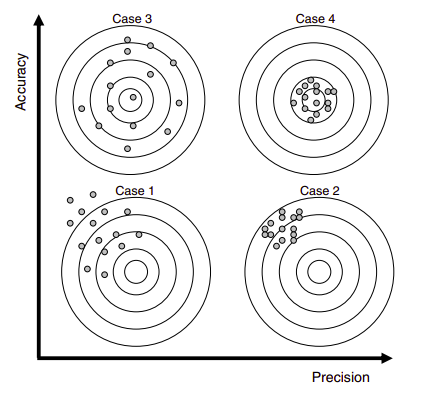
\includegraphics[width=180px]{img/tadeshi_casos.png}
	\caption{Esquematización de Exactitud y Precisión. Fuente: Tedeschi (2006).}
	\label{fig:EsquemaExacPreci}
\end{figure}
\FloatBarrier

De manera similar, la Figura \ref{fig:ComparmedidExacPreci} representa los conceptos ilustrados en la Figura \ref{fig:EsquemaExacPreci} en una forma numérica; el eje $X$ y el eje $Y$ representan al modelo de los valores predichos contra los observados respectivamente. El caso 1 es inexacto e impreciso, el caso 2 es inexacto y preciso, el caso 3 es exacto e impreciso y el caso 4 es exacto y preciso. La línea punteada representa la línea de $X = Y$ . En un modelo de predicción lo ideal es que cumpla el caso 4. 

\begin{figure}[H]
	\centering
	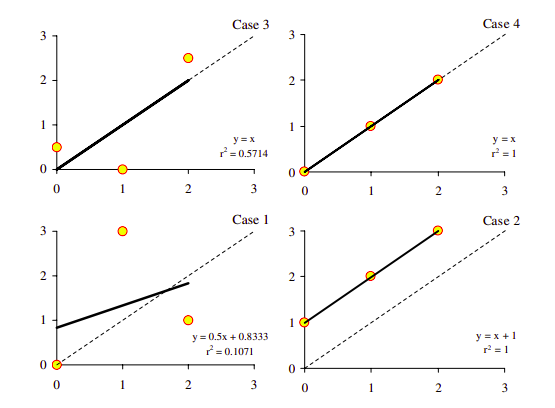
\includegraphics[width=0.6\linewidth]{img/tedeshi_casos_2.png}
	\caption{ Comparación de las medidas de Exactitud y Precisión. Fuente: Tedeschi (2006).}
	\label{fig:ComparmedidExacPreci}
\end{figure}
\FloatBarrier

Las estimaciones del intercepto y la pendiente son buenos indicadores de la exactitud: cuanto mas cerca
estén simultáneamente de cero y uno respectivamente mayor es la exactitud. La estimación del coeficiente de
determinación $(R^{2})$ es un buen indicador de la precisión: cuanto mayor es la $R^{2}$ mayor es la precisión \parencite{balam-2012}.
\vspace{.5cm}

Por su parte, \textcite{mayer-butler-1993} indican que la prueba $t$ paramétrica de medias y el análisis de regresión lineal de la grafica observada frente a la predicha son los métodos estadísticos generales mas útiles, sin embargo, cada método inferencial se encuentra principalmente sujeto a las dificultades para satisfacer sus supuestos.
\vspace{.5cm}



\subsection{Regresión Lineal Simple}
Una de las técnicas mas comunes en la validación de modelos es la de Regresión Lineal Simple de los observados sobre los predichos (Mayer et al., 1994; Analla, 1998; Tedeschi, 2006).
\vspace{.5cm}


El análisis de regresión lineal tiene como objetivo modelar en forma matemática el comportamiento de una variable de respuesta en función de una o mas variables independientes
(Gutiérrez y de la Vara, 2012). Por lo tanto, se ajusta el modelo  $ y_{i} = \beta_{0} + \beta_{1}z_{i} +\epsilon $ donde $ 1 \leq i \leq n$, $ y_{i}$ es el valor real observado en la i-esima unidad experimental, $ z_{i}$ es el correspondiente valor predicho por el modelo a validar, $\epsilon_{i}$ es el componente aleatorio o error, $\beta_{0}$ es la ordenada al origen y $\beta_{1}$ la pendiente \parencite{zacarias-2023}.
\vspace{.5cm}


Esta técnica se encuentra principalmente sujeta al cumplimiento de sus supuestos. Cuando los residuales son independientes, se ajustan a una distribución normal y tienen varianza común, se aplican pruebas de hipótesis estadísticas para evaluar la exactitud, intercepto cero y pendiente uno, ya sea mediante pruebas t de Student, o bien, mediante una prueba F para determinar si el intercepto y la pendiente son simultáneamente cero y uno respectivamente \parencite{balam-2012}.




\subsubsection{Validación de Modelos con la Técnica de Regresión Lineal Simple \parencite{febles-2014}}

\textcite{febles-2014}, describe la validación de modelos con la técnica de regresión lineal simple que se centra en determinar el grado de exactitud y precisión del modelo basándose en el trabajo previo de \textcite{balam-2012}.\\

Sea un modelo $Y = H(\Theta )$, con una muestra pareada $(z_{1}, y_{1}), (z_{2}, y_{2}) , \dots , (z_{n}, y_{n})$ de valores observados y predichos respectivamente por el modelo. Bajo estas condiciones, se considera el modelo de regresión lineal: $y_{i}= \beta_{0} + \beta_{1}z_{i}$, donde $ 1 \leq i \leq n$. Donde  los estimadores de mínimos cuadrados para $\beta_{0}$,  $\beta_{1}$ y el coeficiente de determinación $R^{2}$ son respectivamente: \\

\begin{center}
	$\hat{\beta_{0}} = \hat{y} - \hat{\beta_{1}} \bar{z} $, \\
\end{center}

\begin{center}
	$ \hat{\beta_{1}} = \frac{\sum_{i=1}^{n} (z_{i} - \bar{z} ) (y_{i} - \bar{y})} {  \sum_{i=1}^{n} (z_{i} - \bar{z} )^{2} }$, \\
\end{center}

\begin{center}
	$R^{2} = \frac{ \sum_{i=1}^{n} ( \hat{y}_{i} - \bar{y})^{2}} { \sum_{i=1}^{n} ( y_{i} - \bar{y})^{2}  }$  y  $ 0 \leq R^{2} \leq 1$,
\end{center}


Donde $ \bar{z}$ y $ \bar{y}$ son las medias muéstrales de los valores observados y predichos respectivamente por el modelo; la evaluación estadístico de la exactitud y precisión depende del cumplimiento de los supuestos de normalidad y de varianza constante de los errores i en el modelo. \\


Los residuales $\epsilon_{i} = y_{i} - \bar{y}_{i}$ son estimaciones de los errores $i$ en el modelo, verificando el  supuesto de normalidad en los residuales $\epsilon_{1}, \epsilon_{2} , \dots, \epsilon_{n} $, con pruebas de bondad de ajuste, como la de Kolmogorov-Smirnov y Shapiro Wilk. El supuesto de varianza constante se verifica con el grafico de dispersión entre los predichos $y_{i}$ y los residuales $\epsilon_{i}$ del modelo. Con todas las combinaciones de los supuestos de normalidad y varianza constante, la evaluación de la exactitud y precisión del modelo $Y = H(\Theta )$ se analizan en los siguientes tres casos: cuando la muestra de residuales es independiente con distribución normal y varianza constante (NVC); cuando la muestra de residuales es independiente con distribución no normal y varianza constante (NNVC) y cuando la muestra
de residuales es independiente con varianza no constante (NVD - NNVD).

\subsubsection{Evaluación de la Exactitud de un Modelo}

Cuando se cumplen los supuestos de la Regresión, la verificación de la exactitud de un modelo puede llevarse a cabo vía dos pruebas t de Student, o bien, mediante una prueba F \parencite{balam-2012}.\\

La Prueba F Conjunta que considera el intercepto y la pendiente de manera conjunta, ambos valores agrupados en un vector de dimensión dos, a diferencia del caso anterior, se compara que el vector de parámetros  sea  contra que no lo sea. Bajo la premisa de que los residuales del modelo entre los observados y predichos cumplen los supuestos de normalidad y varianza constante,la prueba de hipótesis conjunta permite obtener una región de confianza para el vector de parámetros ,en este caso,se dice que el modelo ese exacto cuando la región de confianza conjunta contiene al punto $(0,1)$. \parencite{zacarias-2023}.\\

Para la aplicación de la F conjunta se ajusta el modelo de regresión lineal a simple con los supuestos de que los residuos ajustados se distribuyan normal, son independientes y tienen varianza constante (Ayala,2024).\\

Para la prueba de exactitud mediante la prueba de F conjunta se toma en cuenta lo siguiente \parencite{montgomery-2012}: 

\begin{center}
	$S_{zz} = \sum_{i=1}^{n}z_{i}^{2} - \frac{( \sum_{i=1}^{n} z_{i})^{2}}{n} \;$ ,
	$S_{zy} = \sum_{i=1}^{n}z_{i} y_{i} - \frac{ \sum_{i=1}^{n} z_{i} \sum_{i=1}^{n} y_{i} }{n} \;$,\\
\end{center}

\begin{center}
	$SS_{T} = \sum_{i=1}^{n}y_{i}^{2} - \frac{( \sum_{i=1}^{n} y_{i})^{2}}{n} \;$, $\bar{y} = \frac{1}{n} \sum_{i=1}^{n} y_{i} \; $, $\bar{z} = \frac{1}{n} \sum_{i=1}^{n} z_{i} $ \\
\end{center}


\begin{center}
	$ \hat{\beta_{1}} = \frac{S_{zy}}{S_{zz}}  \;$, $\hat{\beta_{0}} =  \bar{y} - \hat{\beta_{a}} \bar{z}  \; $, $\hat{y} = \hat{\beta_{0}}  + \hat{\beta_{1}}z $ \\
\end{center}

\begin{center}
	$ CME =  \frac{SCE}{n-2} = \frac{ \sum_{i=1}^{n} (y_{i} - \hat{y_{i}} )^{2} }{n - 2 } =  \frac{SS_{T} - \hat{\beta_{1}} S_{zy}}{n -2} $ \\
\end{center}


La Prueba F Conjunta considera un sólo procedimiento que nos permite establecer si un modelo es exacto considerando simultáneamente el intercepto \(\beta_0\) y la pendiente \(\beta_1\), es decir, se prueba si $\bigl(\begin{smallmatrix} \beta_{0} \\ \beta_{1} \end{smallmatrix}\bigr) = \bigl(\begin{smallmatrix}0  \\  1\end{smallmatrix}\bigr) $ estadísticamente. flata qui \\

\textcite{zacarias-2023}, para evaluar la exactitud de un modelo ante los escenarios NNVC, NVD y NNVD, implemento un método que consiste en estimar la distribución de la estadística F a través de muestras Bootstrap robustas propuestas en \textcite{rana-2012}, en donde dependiendo del caso que se presente se implementan los distintos tipos de remuestreos propuestos por \textcite{wu-1986} y \textcite{liu-1988} y a partir de estas construir una región de confianza para el vector de parámetros $ \mathbf{\beta} = (\beta_{0}, \beta_{1})$.\\


\subsubsection{Evaluación de la Precisión de un Modelo}

\textcite{zacarias-2023}, menciona que una parte importante del método de regresión lineal, es que estudia si dicha relación permite realizar estimaciones con una precisión aceptable; por lo que también se considera como un criterio cuantitativo relevante para evaluar la calidad de ajuste de la regresión, el coeficiente de determinación $R^{2}$, que en general se interpreta como la proporción de la variabilidad en los datos observados $y_{i}$, que es explicada por el modelo.\\


\textcite{balam-2012}, utilizó un intervalo de confianza Bootstrap para medir la precisión de un modelo, donde el esquema de remuestreo propuesto depende del cumplimiento o no del supuesto de varianza constante. Cuando se cumple dicho supuesto se emplea un intervalo de confianza Bootstrap de residuales balanceado por el método percentil con sesgo corregido acelerado para evaluar la precisión de un modelo; y cuando no se cumple el supuesto de varianza constante se emplea un intervalo de confianza Bootstrap pareado balanceado por el método percentil con sesgo corregido acelerado.\\

\subsubsection{El Coeficiente de Determinación $R^{2}$}

El coeficiente de determinación $R^{2}$ se utiliza cuando las variables de estudio son cuantitativas y están medidas en una escala de intervalo o razón, siendo una herramienta común para medir el ajuste del modelo a los datos. El valor de $R^{2}$
se interpreta frecuentemente como la proporción de la variación de la variable dependiente explicada por el modelo de regresión lineal simple \parencite{balam-2012}. Sin embargo, es importante señalar que $R^{2}$
presenta varias limitaciones y características que deben ser tomadas en cuenta al evaluar su utilidad.\\


Según lo señalado por \textcite{balam-2012}, algunos puntos clave sobre $R^{2}$:\\

\begin{enumerate} 
	\item $R^{2}$ no mide la magnitud de la pendiente de la recta de regresión ajustada, ni implica que una pendiente grande se corresponda con un valor grande de $R^{2}$. 
	
	\item Es posible obtener un valor grande de $R^{2}$ agregando términos adicionales al modelo, lo que puede no reflejar una mejora real en la calidad del modelo.
	
	\item El valor de $R^{2}$  no mide adecuadamente la relación entre las variables si no existe una relación lineal, por lo que puede ser grande aunque 
	y no tengan una relación lineal significativa. 
	
	\item Un valor elevado de $R^{2}$ no necesariamente implica que el modelo sea un buen predictor, ya que puede estar influenciado por factores no realistas en los datos.
	
	\item En algunos casos, $R^{2}$ puede ser pequeño si el intervalo de las $z$  es demasiado estrecho para detectar una relación significativa con $y$. 
	
	\item En presencia de valores atípicos o agrupamientos (clustering) en los datos, $R^{2}$ puede ser engañoso, pues un valor grande podría ser el resultado de estos factores, en lugar de un ajuste verdadero. \\
\end{enumerate}


A pesar de sus limitaciones,  $R^{2}$ tiene ciertas ventajas, como cuando su valor es cercano a cero, lo que indica que el modelo no se ajusta bien a los datos. Sin embargo, si no hay puntos repetidos, es posible construir un modelo polinómico de grado $n-1$ que ofrezca un ajuste perfecto, lo que también pone en evidencia la necesidad de interpretar  $R^{2}$ con cautela.\\

Entre otras características, se destaca que el valor esperado de  $R^{2}$ puede aumentar o disminuir dependiendo de la variabilidad de la variable independiente 
$z$, y que, debido a la falta de conocimiento sobre su distribución exacta,  $R^{2}$  no debe usarse para hacer predicciones directas.\\


Dadas estas limitaciones, es importante considerar estudios adicionales que profundicen en las propiedades de $R^{2}$. \textcite{Ohtani-2004}, mencionan que para medir la precisión de un modelo de regresión lineal simple, al utilizarse tradicionalmente el coeficiente de determinación  \( R^2 \) y el coeficiente de determinación ajustado, se han presentado estudios sobre las propiedades de muestras pequeñas de \( R^2 \) y \( \overline{R}^2 \) como lo son \textcite{barten-1962} que sugiere una versión modificada de \( R^2 \) para reducir su sesgo, y la propuesta de \textcite{crammer-1987} al derivar las fórmulas exactas para los dos primeros momentos de \( R^2 \) y \( \overline{R}^2 \), quien muestra que \( R^2 \) está seriamente sesgado hacia arriba en muestras pequeñas, mientras que \( \overline{R}^2 \) es más inestable que \( R^2 \) en términos de desviación estándar.\\


Por lo cual, en \textcite{Ohtani-2004} deriva las fórmulas exactas para la función de densidad, la función de distribución y el momento \(m\)-ésimo, realizando un análisis numéricos basados en las fórmulas exactas, todo esto considerando un modelo de regresión lineal donde los términos de error obedecen a una distribución \(t\) multivariada, examinando los efectos del alejamiento de la normalidad de los términos de error en las distribuciones exactas de \(R^2\) y \(\bar{R}^2\). Con intervalos de confianza de \(R^2\) y \(\bar{R}^2\), muestran que el sesgo hacia arriba de \(R^2\) se vuelve significativo y que el error estándar de \(R^2\) aumenta a medida que los grados de libertad de la distribución de error \(t\) multivariada (\(\nu_0\)) disminuyen. También se muestra que, cuando los valores de \(\nu_0\) y el coeficiente de determinación de la población (\(\Phi\)) son pequeños, los límites superiores de confianza de \(R^2\) y \(\bar{R}^2\) son muy grandes.\\

Adicionalmente, \textcite{christou-2005} explica la distribución del coeficiente de determinación muestral en el caso de regresión simple utilizando su relación con la distribución \(F\) no central. Introduce el concepto de coeficiente de determinación verdadero, el cual es útil en estudios de simulación donde la varianza del término de error es conocida, permitiendo construir relaciones con una fuerza predeterminada.\\



\subsubsection{Verificación de los Supuestos de Normalidad y Varianza constante}




\subsection{Regresión Lineal Robusta}
En un modelo de regresión lineal, los supuestos de normalidad y homocedasticidad son fundamentales para garantizar la validez de los estimadores obtenidos por mínimos cuadrados ordinarios (OLS). Sin embargo, en la práctica, estos supuestos rara vez se cumplen debido a la presencia de valores atípicos, heterocedasticidad o discrepancias en las hipótesis del modelo. En estos casos, los estimadores de regresión robusta se presentan como una alternativa confiable, ya que están diseñados para ser menos sensibles a dichas anomalías y proporcionar inferencias más confiables sobre los parámetros del modelo \parencite{zacarias-2023}.\\

\textcite{annalisa-2024}, menciona que la regresión robusta ofrece ventajas significativas frente a métodos como la regresión ponderada basada en mínimos cuadrados iterativamente reponderados (IRWLS), especialmente en contextos con patrones heterocedásticos en los residuos. No solo permite gestionar de manera óptima los valores atípicos, sino que también proporciona un enfoque más eficaz para manejar la heterocedasticidad y las desviaciones de los supuestos clásicos del modelo.\\


El objetivo principal de la regresión robusta es desarrollar métodos que produzcan estimaciones precisas y resistentes a influencias indebidas en los datos. Una de las métricas clave para evaluar la robustez de un estimador es el punto de ruptura, definido como la mínima fracción de datos atípicos necesarios para invalidar completamente el estimador. Mientras que los estimadores clásicos como OLS tienen un punto de ruptura bajo que converge a cero a medida que aumenta el tamaño de la muestra, los estimadores robustos modernos pueden alcanzar un punto de ruptura de hasta el 50\%, lo que los hace altamente resistentes ~\parencites{siegel-1982,rousseeuw-1984}. \\

Entre los estimadores robustos más avanzados se encuentra el MM-Estimador, introducido como una combinación de alta eficiencia y robustez.El MM-Estimador es especialmente útil en contextos donde los datos contienen una proporción significativa de valores atípicos, ya que logra una eficiencia asintótica superior al 85\% y un punto de ruptura máximo del 50\% \parencite{rousseeuw-yohai-1984}. Este balance lo convierte en una herramienta clave para análisis estadísticos robustos, asegurando un ajuste confiable incluso en condiciones adversas.\\



\subsubsection{MM-Estimador \parencite{yohai-1987}}
El estimador MM tiene las siguientes propiedades: (i) es altamente eficiente cuando los errores tienen una distribución normal y (ii) su punto de ruptura es 0.5.\\

El estimador MM se define en un procedimiento de tres etapas. En la primera etapa, se calcula una estimación de regresión inicial que es consistente, robusta y con un alto punto de ruptura, pero no necesariamente eficiente. En la segunda etapa, se calcula un estimador M de la escala de errores utilizando residuos basados en la estimación inicial. Finalmente, en la tercera etapa se calcula un estimador M de los parámetros de regresión basada en una función $\psi$ descendente.\\

Considerando el modelo de regresión lineal simple:
\begin{center}
$y_{i}= \beta_{0} + \beta_{1}z_{i}$, $1 \leq i \leq n, $
\end{center}

\textcite{huber-1981} define los estimadores M de la siguiente manera: Sea una función real que satisfaga los siguientes supuestos (A1):

\begin{enumerate}[label=\roman*.]
	\item $\rho(0) = 0$.
	\item   $\rho(-u) =  \rho(u)$.
	\item $1 \leq i \leq v$ implica $\rho(u) \leq  \rho(v)$.
	\item $\rho$ es continua.
	\item Sea a = sup $\rho(u)$, entonces $0<a< \infty$.
	\item Si $\rho(u) < a $ y $0 \leq  u < v $, entonces  $\rho(u) <  \rho(v)$.
\end{enumerate}

Dada una muestra de tamaño $n$, $ \mathbf{u} = (u_{1}, u_{2}, \dots , u_{n})$,  el estimador M, $s(\mathbf{u})$ está de nido como el valor de s que es la solución de\\

\begin{center}
	$\frac{1}{n} \sum_{i=1}^{n} \rho( \frac{u_{i}}{s}) = b$,\\
\end{center}

donde $b$ puede de definirse como $E_{\Phi}(\rho(u)) = b$, donde $\Phi$ denota la distribución normal estándar.\\

Se cumple que si $c(\mathbf{u}) = \#\{i : 1 \leq i \leq n, u_{i}=0\} / n < 1- (b/a) $, entonces la sumatoria previa tiene solución única y esta solución es diferente de 0. Si $c(\mathbf{u}) \geq 1 -  (b/a)$, se define $s(\mathbf{u}) = 0$. \\

Luego, el estimador MM se define en tres etapas de la siguiente manera:\\

\begin{enumerate}
	\item Sean $ \beta_{0}^{'}$ y $ \beta_{1}^{'}$ estimaciones de los parámetros$ \beta_{0}$ y $ \beta_{1}$ respectivamente con un alto punto de ruptura, posiblemente 0.5.
	\item  Calcular los residuales\\
	\begin{center}
		 $ \epsilon_{i} = y_{i} -\beta_{0}^{'} -\beta_{1}^{'} z_{i}  $, $1 \leq i \leq n $.\\
	\end{center}
	
	y calcular $s_{n} = s(\epsilon_{i})$, el estimador M definido previamente, usando una función $\rho_{0}$ que satisface los supuestos (A1) y considerando una constante $b$ tal que $b/a = 0.5$, donde$ a = $ máx $ \rho_{0}(u)$, lo cual implica que para esta escala la estimación tiene un
	punto de ruptura igual a 0.5.
	
	\item  Sea $\rho_{1}$ otra función que satisfaga los supuestos (A1) y tal que\\
	\begin{center}
		$\rho_{1}(u) \leq \rho_{0}(u)$\\
		sup $\rho_{1}(u)$  = sup $ \rho_{0}(u) = a$\\
	\end{center}

	
	Sea $\psi_{1} = \rho_{1}^{'}$. Entonces el estimador MM, se define como cualquier solución de\\
	\begin{center}
		$\sum_{i=1}^{n} \psi_{1} (\frac{\epsilon_{i}}{s_{n}}) z_{i} = 0$\\
	\end{center}

\end{enumerate}


\subsubsection{ Algoritmo MM-Estimador \parencite{zacarias-2023} }
Como se presenta en la tesis de \textcite{zacarias-2023}, el algoritmo MM-Estimador es un enfoque robusto que mejora la estimación de los coeficientes en presencia de valores atípicos. A continuación, se describe el algoritmo:\\

Sea\\
\begin{center}
 $ y_{i} = \beta_{0} -\beta_{1}z_{i} + \epsilon_{i} $, $1 \leq i \leq n $,\\
\end{center}

una muestra de tamaño $n$ y suponga dadas las estimaciones iniciales $\beta_{0}^{'}$ y $\beta_{0}^{'}$, además del estimador M definido en la Etapa 2 como $s_{n}$. Para cada $t \: \in  \: \mathbb{R} $ se definen los pesos
$w_{i}(t) = \psi_{1} (\epsilon_{i} /s_{n}) /(\epsilon_{i} /s_{n})$. También se definen \\


\begin{center}
	$g(t) = \frac{1}{s_{n}^{2}} \sum_{i=1}^{n} w_{i}( t )\epsilon_{i} z_{i} =  \frac{1}{s_{n}}  \sum_{i=1}^{n} \psi_{1} (\frac{\epsilon_{i}}{s_{n}}) z_{i} $, y \\	
\end{center}

\begin{center}
	$ M(t) = \frac{1}{s_{n}^{2}}  \sum_{i=1}^{n}  w_{i}( t ) z_{i}^{2} $.\\
\end{center}





Si $t^{(i)}$ es el valor de la estimación en la j-esima iteración, entonces $t^{(j+1)}$ está definido por $t^{(j+1)} = t^{(j)} + \Delta ( t^{(j)})$, donde,\\

\begin{center}
	$\Delta ( t) = M^{-1}(t)g(t)$.\\
\end{center}

Sea $0< \delta  < 1$  y $-g(t)$ el gradiente de $S(t)$, donde \\

\begin{center}
	$S(t) = \sum_{i=1}^{n} \rho_{1} ( \frac{\epsilon_{i}}{s_{n}})$. \\
\end{center}


Es posible encontrar un entero $k$ \parencite{yohai-1987} tal que\\

\begin{center}
	$ S(t^{(j)} + \Delta(t^{(j)} )/2^{k}) \leq S(t^{(j)}) - \delta( \Delta(t^{(j)} )/2^{k} ) g(t^{(j)})$. \\
\end{center}


Sea $k_{1,j}$ el mínimo de dichas $k$ y sea $k_{2,j}$ el valor de $k, 0 \leq k  \leq k_{1,j}$, lo que da el mínimo de $S(t^{(j)} + \Delta(t^{(j)} )/2^{k})$. Entonces se define el paso recursivo mediante\\

\begin{center}
	$ t^{(t+1)} = (t^{j} + (1/2^{k_{2,j}}) \Delta(t^{(j)} )$.\\
\end{center}

comenzando $t_{(0)} $ las estimaciones de los parámetros de regresión $\beta_{0}$ y $\beta_{1}$.\\

Los estimadores MM considerados se basan en la función $\rho$ bicuadrada dada por:


\[
\rho(u) =
\begin{cases}
	u^{2}/2 -u^{4}/2 + u^{6}/6	, & \text{si } |u| \leq 1 \\ \\
	1/6,     & \text{si } | u | > 1\\
\end{cases}
\]


que corresponde a la función $\psi$ bicuadrada

\[
\psi(u) =
\begin{cases}
	u(1- u^{2})^{2}	, & \text{si } |u| \leq 1 \\ \\
	0,     & \text{si } | u | > 1
\end{cases}
\]



\subsection{La Técnica Bootstrap}

La Técnica Bootstrap es un método computacional intensivo que permite simular la distribución de una estadística. La idea es maestrear repetidamente los datos observados, produciendo cada vez una función de distribución empírica a partir de los datos remuestreo dos \parencite{zacarias-2023}. El Bootstrap se desarrollo por primera vez para datos independientes y distribuidos de manera idéntica, pero esta suposición se puede relajar para que sea posible realizar
estimaciones de Bootstrap a partir de datos dependientes, como los residuos de regresión o los datos de series de tiempo (Givens y Hoeting, 2013).\\


El enfoque Bootstrap esta especialmente indicado en los casos en donde los datos no siguen una distribución normal, hecho que es común a la mayor parte de las medidas utilizadas habitualmente en las ciencias del comportamiento (Micceri, 1989).\\


El Bootstrap constituye una variedad de técnicas para la inferencia estadística denominadas genéricamente métodos de remuestreo entre las que se encuentran la permutación estocástica, el Jacknife y la validación cruzada (Balam, 2012). Con los métodos de remuestreo nos permiten cuantificar la incertidumbre calculando errores estándar e intervalos de confianza y realizando pruebas de significancia.Requieren menos suposiciones que los métodos tradicionales y generalmente dan respuestas precisas (Hesterberg et al. , 2003).\\


Segun Hesterberg et al., (2003) las ventajas del bootstrap son:

\begin{enumerate}
	\item  Pocos supuestos. No requiere que la muestra sea modelada con la distribución normal o que el tamaño de muestra sea grande.
	
	\item Mayor precisión. Algunos métodos Bootstrap son mas precisos en la practica que los métodos clásicos.
	
	\item Generalidades. Los métodos de remuestreo son notablemente similares para una amplia gama de estadísticos y no requieren de nuevas formulas para cada estadístico. No es necesario memorizar o buscar formulas especiales para cada procedimiento.
\end{enumerate}


\subsubsection{El Principio Bootstrap}
Sea $\theta =T(F)$ una característica de interés de una distribución $F$ desconocida. Sea $x_{1}, x_{2}, \dots, x_{n}$ aleatoria independiente e idénticamente distribuida de la distribución $F$, sea $\chi =\{ x_{1}, x_{2}, \dots, x_{n} \}$ junto de datos y sea $\hat{F}(x) = \frac{1}{n} \sum_{i=1}^{n} I _{(-\infty, x)} (x_{i})$ la distribución empírica de la muestra. Entonces un estimador de $\theta$ es $\hat{\theta} = T(\hat{F})$ (Givens y Hoeting, 2005).\\

Suponga que se desea estimar la distribución $F$ de $\hat{\theta}$ la distribución $F_{R}$ de algún estadístico de prueba $R( \chi, F)$. Por ejemplo, un estadístico de prueba es\\

\begin{center}
	$ R( \chi, F) = [T(\hat{F}) - T(F)/S(\hat{F})]$\\
\end{center}

donde $S(\hat{F})$ estima la desviación estándar de $T(\hat{F})$. La distribución de la variable aleatoria $R( \chi, F)$ puede ser intratable o completamente desconocida. Esta distribución también puede depender de la distribución desconocida de $F$. Ante esta situación, la metodología Bootstrap proporciona una aproximación a la distribución de $R( \chi, F)$ derivada de la función de distribución empírica de los datos observados de manera numérica \parencite{balam-2012}.\\

A continuación, se detallan algoritmos Bootstrap implementados por \textcite{balam-2012}:\\

\subsubsection{Algoritmo de Remuestreo Básico \parencite{balam-2012}}

Se asume una muestra de $ x_{1}, x_{2},  \dots,  x_{n}$ independiente e idénticamente distribuida.

\begin{enumerate}
	\item Se obtienen $B$ muestras de tamaño $n$ con reemplazo y con probabilidades iguales de la muestra original. La cardinalidad de este espacio muestra es $n^{n}$. Se denotan las muestras Bootstrap por $X^{*}_{1}, X^{*}_{2},  \dots, X^{*}_{B}$ donde cada $X^{*}_{i}$ es un vector de tamaño $n$.
	
	\item Se obtienen las muestras, $\hat{\theta}^{*}_{1} = T (X^{*}_{1}) , \hat{\theta}^{*}_{2} = T (X^{*}_{2}), \dots,\hat{\theta}^{*}_{B} = T (X^{*}_{B})$.
	
	\item Se usa la distribución empírica $\hat{F}_{\hat{\theta}^{*}}$ de la muestra $\hat{\theta}^{*}_{1},\hat{\theta}^{*}_{2},  \dots, \hat{\theta}^{*}_{B}$ para estimar $F_{\hat{\theta}} $.
\end{enumerate}

En la practica, se usa una $B$ grande para disminuir el error de simulación al evitar el calculo de todo el espacio muestra Bootstrap.\\

Las estimaciones para  $F_{\hat{\theta}}, \theta^{*}$ y $ \sigma_{\theta^{*}} $ están dadas respectivamente por:

\[
\hat{F}_{\hat{\theta}^{*}} \approx F_{\hat{\theta}}, 
\hspace{.5cm} \hat{\theta}^{*} = \frac{1}{B} \sum_{i=1}^{B}  \hat{\theta}^{*}_{i} \approx \theta,
\hspace{.5cm} Var(\hat{\theta}^{*}) = \frac{1}{B-1} \sum_{i=1}^{B}(\hat{\theta}^{*}_{i}-\hat{\theta}^{*})^2
\]




\subsubsection{Algoritmo de Remuestreo Balanceado \parencite{balam-2012}}
\textcite{balam-2012}, menciona que el Bootstrap Balanceado al ser una modificación a la forma del muestreo del Bootstrap básico garantiza que los datos correspondientes a cada individuo de la muestra aparezcan el mismo numero de veces, incrementando con esto la eficiencia.\\

Se asume una muestra  $ x_{1}, x_{2},  \dots,  x_{n}$ independiente e idénticamente distribuida y supongamos que se desean obtener $B$ muestras Bootstrap.

\begin{enumerate}
	\item  Considere el vector $ X=(x_{1}, x_{2},  \dots,  x_{n}) $.
	
	\item  Generar un vector $ N= (1,2,\dots,n,1,2,\dots,n,1,2,\dots,n)$ de longitud $nB$.
	
	\item Generar una permutación aleatoria $N^{*}$ del vector $N$.
	
	\item La muestra Bootstrap haciendo lo siguiente:
	
	$X^{*}_{1}$ =  Los elementos de $X$ comprendidos desde la primera hasta la posición $n$ de $N^{*}$.\linebreak
	$X^{*}_{2}$ =  Los elementos de $X$ comprendidos desde la posición $n + 1$ hasta la posición $2n$ de $N^{*}$.\\
	\vdots\\
	$X^{*}_{B}$ =  Los elementos de $X$  cuyas posiciones son las ultimas $n$ posiciones de $N^{*}$.
	
	\item  Se obtienen las muestras, $\hat{\theta}^{*}_{1} =T (X^{*}_{1}), \hat{\theta}^{*}_{2} =T (X^{*}_{2}), \dots, \hat{\theta}^{*}_{B} =T (X^{*}_{B})$.
	
	\item  Se usa la distribución empírica $\hat{F}_{\hat{\theta}^{*}}$ de la muestra $\hat{\theta}^{*}_{1},\hat{\theta}^{*}_{2}, \dots, \hat{\theta}^{*}_{B}$ para estimar $F_{\hat{\theta}}$
	
\end{enumerate}



\subsubsection{Bootstrap en Regresión Lineal}

Sea $(y_{i}, z_{i}),  1 \leq  i \leq n$; una muestra pareada entre observados y predichos, se define el modelo de regresión lineal, $ y_{i} = \beta_{0} + \beta_{1}z_{i} +\epsilon $, teniendo con Bootstrap la idea de  estimar la distribución de la estadística $R( \chi, \theta)$ que esta en función de $\theta = (\beta_{0}, \beta_{1}) $ y de $\hat{\theta}$ \parencite{zacarias-2023}. Hay dos maneras de aplicar el Bootstrap
en un modelo de regresión: aplicando Bootstrap a la muestra de residuales o aplicando Bootstrap a la muestra Pareada entre Y y Z \parencite{balam-2012}.\\


\subsubsection{Algoritmo Bootstrap de Residuales}

Se asume que los $ \epsilon_{i} $ son independientes e idénticamente distribuidos. El algoritmo Bootstrap para generar muestras de $ R^{2} $ es el siguiente:

\begin{enumerate}
	\item Ajustar una regresión simple para el modelo $ y_{i} = \beta_{0} +\beta_{1}x_{i} + \epsilon_{i} $.
	
	\item Obtener los residuales $ \epsilon_{i} = y - \hat{y}   $
	, $i = 1,2,\dots, n $.
	
	\item  Remuestrear con probabilidades iguales la muestra $ e_{1},\dots,e_{n} $, para obtener $e^{*}_{11},...,e^{*}_{1n}$.
	\item Obtener $ y^{*}_{1i} = e^{*}_{1i} + \hat{y}_{1i}, i = 1,2, \dots, n. $.
	
	\item Correr una regresión simple $ y^{*}_{1i} = \beta^{*}_{10} +\beta^{*}_{11}x_{i} + \epsilon^{*}_{1i} $ para obtener $ \hat{R}^{2*}_{1} $.
	
	\item Repetir los pasos 3 al 5, $B - 1$ veces para obtener las muestras: 
	\[
	\hat{R}^{2*}_{1} \hspace{.5cm} \hat{R}^{2*}_{2} \hspace{.5cm} \dots \hspace{.5cm} \hat{R}^{2*}_{B}
	\]
\end{enumerate}



\subsubsection{Algoritmo Bootstrap Pareado}

Se asume que los los $e_{i}$ en el modelo
$ y_{i} = \beta_{0} +\beta_{1}x_{i} + \epsilon_{i}$, $i=1,2,..., n$ , no tienen varianza constante, lo que implica que no son idénticamente distribuidos (Givens y Hoeting, 2005; Montgomery et al., 2006).

\begin{enumerate}
	\item Considere la muestra $ w_{1} = (y_{1}, x_{1}),  w_{2} = (y_{2}, x_{2}), ..., w_{n} = (y_{n}, x_{n})$ como una muestra independiente e idénticamente distribuida donde la distribución es la conjunta $ F_{Y|X} $.
	
	\item  Tomar una muestra Bootstrap  $ w^{*}_{1}, w^{*}_{2},...,  w^{*}_{n} $ de $w_{1}, w_{2},...,  w_{n} $. Se obtienen la muestras  $y_{1}, y_{2},...,  y_{n} $ y  $x_{1}, x_{2},...,  x_{n} $.
	
	\item Correr una regresión lineal $ y^{*}_{i} = \beta_{i0} +\beta_{i1}x_{i}^{*} + \epsilon_{i} $.
	
	\item Estimar  $ \hat{R}^{2*}_{1} $.
	
	\item  Repetir los pasos 3 al 5, $B - 1$ veces para obtener las muestras: 
	\[
	\hat{R}^{2*}_{1} \hspace{.5cm} \hat{R}^{2*}_{2} \hspace{.5cm} \dots \hspace{.5cm} \hat{R}^{2*}_{B}
	\]
\end{enumerate}


\subsubsection{Algoritmo Bootstrap Robusto Simple}
El algoritmo Bootstrap para generar muestras Bootstrap robustas para $\hat{R}^{2}$ es el siguiente:

\begin{enumerate}
	\item Obtener el MM-Estimador $\hat{B}^{MM}$ de $B$ ... y con este  obtener los ajustados $ \hat{y}^{MM}_{i} = z_{i}B^{MM},i=1,2,..., n$.
	
	\item Obtener los residuales del modelo robusto $ e^{MM}_{i} = y_{i}-\hat{y}^{MM}_{i},i = 1,2, \dots, n$.
	
	\item Remuestrea con reemplazo y con probabilidades la muestra robusta $ e^{MM}_{1},\dots, e^{MM}_{n}$ para obtener $ e^{*MM}_{1},\dots, e^{*MM}_{n}$.
	
	\item Obtener $y^{*MM}_{i} = e^{*MM}_{i} + \hat{y}^{MM}_{i},i=1,2,..., n  $.
	
	\item Ajustar una regresión simple $ y^{*MM}_{i} = \beta_{0}^{*MM}+\beta_{1}^{*MM}z_{i} + e^{*MM}_{1i}$ y obtener $\hat{R}^{2*MM}_{1}$
	
	\item Repetir los pasos 3 a 5, $(B-1)$ veces para obtener las muestras Bootstrap:
	
	\[
	\hat{R}^{2*MM}_{1} \hspace{.5cm} \hat{R}^{2*MM}_{2} \hspace{.5cm} \dots \hspace{.5cm} \hat{R}^{2*MM}_{B}
	\]
\end{enumerate}



\subsection{Wild Bootstrap}
El Wild Bootstrap es una técnica útil cuando no se cumplen los supuestos de homocedasticidad en modelos de regresión. \textcite{wu-1986} demostró que, en presencia de heterocedasticidad, las estimaciones de mínimos cuadrados son inconsistentes y asintóticamente sesgadas. Para abordar este problema, propuso un esquema Bootstrap basado en tres métodos de remuestreo de residuales, mejorando así la precisión de las estimaciones de los parámetros del modelo. Posteriormente, \textcite{liu-1988} amplió el trabajo de Wu al desarrollar dos alternativas adicionales para generar remuestras de residuales. \\


\textcite{russell-2008} en su estudió sobre el Wild Bootstrap en modelos de regresión con perturbaciones heterocedásticas, demostraron que en casos específicos, puede lograrse una inferencia perfecta. Aunque ciertas versiones carecen de corrección de asimetría, han mostrado reducciones significativas en errores de probabilidad de rechazo en pruebas Bootstrap, incluso en muestras pequeñas o medianas.\\

Estudios posteriores, como el de \textcite{rana-2012}, implementaron algunos de los esquemas de Wu y Liu; y demostraron que ofrecen un rendimiento superior en comparación con métodos tradicionales como el Bootstrap clásico, especialmente cuando existen valores atípicos. La asignación de pesos a los residuales estabiliza la varianza de las estimaciones, lo que resulta crucial para obtener inferencias más confiables.\\


Finalmente, \textcite{zacarias-2023} aplicó estos esquemas de Wild Bootstrap para evaluar la exactitud de modelos de regresión lineal en situaciones donde los supuestos de normalidad o varianza constante no se cumplen. Con una metodología inédita que utilizó los tres esquemas propuestos por \textcite{wu-1986} y las dos variantes de \textcite{liu-1988} para construir regiones de confianza robustas, adaptándose a diferentes escenarios de residuales.\\


En los apartados siguientes, se detallarán los algoritmos del Bootstrap robusto propuesto \textcite{rana-2012} con las tres diferentes maneras de remuestreo propuesto en \textcite{wu-1986} y con las dos formas
propuestas en \textcite{liu-1988}.



\subsubsection{Técnica Robusta Basada en el Esquema Wild Bootstrap}

\textbf{Algoritmo - Esquema Bootstrap de Wu 1}

\begin{enumerate}
	\item  Ajustar un modelo $y_{i} = \beta_{0} +\beta_{1}z_{i} + \epsilon_{i}$  mediante el MM-estimador de la muestra original de observaciones para obtener los parámetros robustos $\hat{B}^{MM}$ y, obtener los ajustados $\hat{y}_{i}=z_{i}\hat{\beta}_{MM}$.
	
	\item  Calcular los residuales $ \hat{e}^{MM}_{i} = y_{i}-\hat{y}_{i},i = 1,2, \dots, n$, y obtener los residuales ponderados
	\begin{center}
	\[
	\hat{e}^{WMM}_{i} =
	\begin{cases}
		e^{MM}_{i}, & \text{si } \frac{|e^{MM}_{i}|}{\sigma_{MM}} \leq c \\ \\
		\frac{c \times e^{MM}_{i}}{ | \hat{e}^{MM}_{i} | /\sigma_{MM}},     & \text{si } \frac{|e^{MM}_{i}|}{\sigma_{MM}} > c
	\end{cases}
	\]
	\end{center} 
	donde $c$ es una constante arbitraria que se elige entre 2 y 3; mientras que $\sigma_{MM}$ es la
	raíz cuadrada del cuadrado medio del error del modelo robusto $\sigma_{MM} = \sqrt{CME}$.

	\item Obtener una muestra Bootstrap $y^{*}_{i}$, tal que 
	\begin{center}
		$y^{*}_{i} =z_{i}\hat{\beta}_{MM} + \frac{t^{*}_{i}\hat{e}^{WMM}_{i}}{\sqrt{1-h_{ii}}} $,
	\end{center}
	donde $h_{ii}$ es el i-ésimo elemento de la matriz diag$(Z(Z^{T}Z)^{-1} Z^{T})$ y el valor $t^{*}_{i}$ es el
	i-ésimo elemento de una muestra aleatoria de tamaño $n$ de una $N(0,1)$.
	
	\item  Ajustar una regresion simple $ y^{*}_{1i} = \beta^{*}_{10} +\beta^{*}_{11}x_{i} + \epsilon^{*}_{1i} $ para obtener $ \hat{R}^{2*}_{1} $.
	
		\item Repetir $B - 1$ veces veces los pasos 3 y 4 para obtener las muestras:
	\[
	\hat{R}^{2*}_{1} \hspace{.5cm} \hat{R}^{2*}_{2} \hspace{.5cm} \dots \hspace{.5cm} \hat{R}^{2*}_{B}
	\]
\end{enumerate}


\textbf{Algoritmo - Esquema Bootstrap de Wu 2}

\begin{enumerate}
	\item Repetir los pasos 1 y 2 del Algoritmo Wu 1.
	
	\item  Similar al paso 3 del Algoritmo Wu 1,se obtiene una muestra Bootstrap;
	pero el valor $t^{*}_{i}$ es el i-ésimo elemento de una muestra con reemplazo con probabilidades iguales de los residuos normalizados $a_{1},a_{2}, \dots,a_{n}$, donde
	
	\begin{center}
		$a_{i} = \frac{\hat{e}_{i}-\bar{\hat{ e}}_{i}}{ \sqrt{ \frac{1}{n} \sum_{i=1}^{n} (\hat{e}_{i}-\bar{\hat{e}})^{2} } }$ con $ \bar{\hat{e}}= \frac{1}{n} \sum_{i=1}^{n} \hat{e}_{i} $.
	\end{center}
	
	\item Repetir los pasos 4 y 5 del Algoritmo Wu 1.
\end{enumerate}



\textbf{Algoritmo - Esquema Bootstrap de Wu 3}

\begin{enumerate}
	\item Repetir los pasos 1 y 2 del Algoritmo Wu 1.
	
	\item  Similar al paso 3 del Algoritmo Wu 1,se obtiene una muestra Bootstrap;
	pero el valor $t^{*}_{i}$ es el i-ésimo elemento de una muestra con reemplazo con probabilidades iguales del vector de residuales transformado:
	
	\begin{center}
		$R_{ai} = \frac{\hat{e}^{WMM}_{i} - Mediana(\hat{e}^{WMM}_{i})}{ NMAD(\hat{e}^{WMM}_{i})  }$ ,
	\end{center}
	donde $NMAD = \frac{1}{0.6745} Mediana\{ | \hat{e}^{WMM}_{i} - Mediana(\hat{e}^{WMM}_{i}) | \}$.
	
	\item Repetir los pasos 4 y 5 del Algoritmo Wu 1.
\end{enumerate}


\textbf{Algoritmo - Esquema Bootstrap de Liu 1}

\begin{enumerate}
	\item Repetir los pasos 1 y 2 del Algoritmo Wu 1.
	
	\item  Similar al paso 3 del Algoritmo Wu 1,se obtiene una muestra Bootstrap;
	pero el valor $t^{*}_{i}$ es el i-ésimo elemento de una muestra aleatoria de tamaño $n$ de una distribución Gamma$(\alpha = 4,\beta = 1/2)$ con función de densidad $ gz(x) = [\frac{2^{4}}{3!}]x^{3}e^{-2x}I_{(x>0)}$ 

	
	\item Repetir los pasos 4 y 5 del Algoritmo Wu 1.
\end{enumerate}



\textbf{Algoritmo - Esquema Bootstrap de Liu 2}

\begin{enumerate}
	\item Repetir los pasos 1 y 2 del Algoritmo Wu 1.
	
	\item  Similar al paso 3 del Algoritmo Wu 1,se obtiene una muestra Bootstrap;
	pero el valor $t^{*}_{i}$ es el i-ésimo elemento de una muestra aleatoria de tamaño $n$ obtenida por 
	
	\begin{center}
		$t^{*}_{i} = H_{i}D_{i}- E(H_{i})E(D_{i})$,\hspace{.5cm} $i = 1,2, \dots, n$
	\end{center}
	
	donde$ H_{1},H_{2}, \dots,H_{n}$ son variables aleatorias independientes, idénticamente normalmente distribuidas con media $(1/2)( \sqrt{17/6})+ \sqrt{1/6}$ y varianza $1/2$. De igual manera,$ D_{1},D_{2}, \dots,D_{n}$ también se distribuyen normal, son independientes e idénticamente
	distribuidas con media $(1/2)( \sqrt{17/6})- \sqrt{1/6}$ y varianza  $1/2$. Tanto $ H_{i}$ y las $ D_{i}$ son independientes entre sí.
	
	\item Repetir los pasos 4 y 5 del Algoritmo Wu 1.
\end{enumerate}



\subsection{Intervalos de Confianza Bootstrap}
Las muestras Bootstrap se pueden utilizar para calcular intervalos de confianza mas aproximados. Cuando $n \rightarrow \infty$, el Bootstrap y el intervalo estándar convergen el uno al otro; en algunas situaciones se pueden hacer correcciones al sesgo. Estas correcciones pueden significativamente mejorar la exactitud inferencial de la estimación de un intervalo \parencite{efron-tibs-1993}.\\


\textcite{good-2005}, determina que el Bootstrap puede ayudarnos a obtener una estimación del intervalo para cualquier aspecto de la distribución si las observaciones son independientes y todos provienen de una distribución con el mismo valor del parámetro que se estima.El Bootstrap es particularmente valioso cuando se trata de obtener una estimación del intervalo para una proporción o para la media y la varianza de una distribución no simétrica.\\


Según \textcite{balam-2012}, desafortunadamente, tales intervalos tienen las siguientes de ciencias:\\

\begin{enumerate}
\item Son sesgados, esto es, es mas probable que contengan ciertos valores falsos del parámetro que se estiman que el verdadero.

\item Son mas anchos y menos eficientes de lo que podrán ser.
\end{enumerate}

Motivos por los que en \textcite{balam-2012} se implementa dos métodos para corregir estas de ciencias, el primero es el método Percentil con sesgo corregido y el segundo es el Bootstrap con sesgo corregido acelerado BCa.\\

Se recomienda que el número de remuestras Bootstrap este entre 2000 y 4000 en orden para la construcción de intervalos de confianza, especialmente para los percentiles mas bajos. Meeker y Escobar (1998).\\

A continuación se presentan los algoritmos para al construcción de intervalos de confianza Bootstrap con el método Percentil de \textcite{efron-1982} y Bootstrap con sesgo corregido acelerado BCa implementado en \textcite{balam-2012}.\\

\subsubsection{Algoritmo Intervalo de Confianza Bootstrap Método Percentil}

Para calcular un intervalo de confianza Bootstrap Percentil de $\hat{\theta}$ a partir de un muestra $x_{1}, x_{2}, \dots, x_{n}$ con probabilidad $(1-\alpha)$\% y con $B$ muestras.


\begin{enumerate}
\item Se obtienen $B$ muestras de tamaño $n$ con reemplazo y con probabilidades iguales de la muestra original. Se denotan las muestras Bootstrap por $X^{*}_{1}, X^{*}_{2},  \dots, X^{*}_{B}$ donde cada $X^{*}_{i}$ es un vector de tamaño $n$.

\item Se obtienen las muestras, $\hat{\theta}^{*}_{1} = T (X^{*}_{1}) , \hat{\theta}^{*}_{2} = T (X^{*}_{2}), \dots,\hat{\theta}^{*}_{B} = T (X^{*}_{B})$.

\item Las $B$ muestras $\hat{\theta}^{*}_{1}, \hat{\theta}^{*}_{2},\dots, \hat{\theta}^{*}_{B} $ se ordenan de manera ascendente, tal que $\hat{\theta}^{*}_{1} \leq \hat{\theta}^{*}_{2} \leq \dots \leq \hat{\theta}^{*}_{B} $.

\item Determinar los cuantiles $LI$ y $LS$, para el nivel de confianza del $(1-\alpha)$\% en la muestra Bootstrap ordenada, con $LI = \hat{\theta}^{*}_{ ( \alpha/2 ) \: \times \: B} $ y $LS = \hat{\theta}^{*}_{ (1 - \alpha/2) \: \times \: B} $.

\item El intervalo de confianza esta dado por: $[LI, LS]$.
\end{enumerate}





\subsubsection{Algoritmo Intervalo de Confianza Bootstrap BCa}

Para calcular un intervalo de confianza Bootstrap BCa de $\hat{\theta}$ a partir de un muestra $x_{1}, x_{2}, \dots, x_{n}$ con probabilidad $(1-\alpha)$\% y con $B$ muestras.


\begin{enumerate}
 \item Obtener una estimación $\hat{\theta}$ a partir de los datos originales.
 
\item Se obtienen $B$ muestras de tamaño $n$ con reemplazo y con probabilidades iguales de la muestra original. Se denotan las muestras Bootstrap por $X^{*}_{1}, X^{*}_{2},  \dots, X^{*}_{B}$ donde cada $X^{*}_{i}$ es un vector de tamaño $n$.

\item Se obtienen las muestras, $\hat{\theta}^{*}_{1} = T (X^{*}_{1}) , \hat{\theta}^{*}_{2} = T (X^{*}_{2}), \dots,\hat{\theta}^{*}_{B} = T (X^{*}_{B})$.

\item Se determina la proporción $p$ de las  $\hat{\theta}^{*}_{i}$ que son mayores o iguales a $\hat{\theta}$.

\item  Determinar $Z_{0} = Z_{p}$ donde $Z_{p}$ es el cuantil en la distribución normal estándar tal que $P(Z > Z_{p}) = p$.

\item  Obtener la constante de aceleración $a$ dada por:
\begin{center}
 \Large $ a = \frac{\sum_{i=1}^{n}  (\hat{\theta}_{-iprom}  - \hat{\theta}_{-i})^{3} }{ 6 \; (\; \sum_{i=1}^{n}  ( \hat{\theta}_{-iprom}  - \hat{\theta}_{-i})^{2} \; )^{3/2}} $
\end{center}

 donde: $\hat{\theta}_{-i}$ es la estimación con los datos originales quitando la $i$-esima observación y {\normalsize $\hat{\theta}_{-iprom} = \frac{1}{n} \sum_{i=1}^{n}\hat{\theta}_{-i}$}
 
 \item Obtener {\large $Z_{L} = \frac{Z_{0} - Z_{\alpha/2}}{ 1- \alpha ( Z_{0} - Z_{\alpha/2})} + Z_{0}  $}   y {\large $Z_{U} = \frac{Z_{0} + Z_{\alpha/2}}{ 1- \alpha ( Z_{0} - Z_{\alpha/2})} + Z_{0}  $}  donde: $Z_{\alpha /2}$ es el cuantil en la
 distribución normal estándar tal que $P(Z > Z_{\alpha / 2}) = \frac{\alpha}{2}$.
 
 
 \item Encontrar $LI = INVCDF( \Phi(Z_{L}))$ y $LS = INVCDF( \Phi(Z_{U}))$ donde $INVCDF$ es el cuantil en la muestra bootstrap con probabilidad $ \Phi(Z_{L})$ y $ \Phi(Z_{U})$ respectivamente y $\Phi$ es la distribución acumulada de la normal estándar, siendo $P(\hat{\theta}^{*} < LI) = \Phi(Z_{L})$ y$P(\hat{\theta}^{*} < LS) = \Phi(Z_{U})$.
 
\item El intervalo de confianza esta dado por: $[LI, LS]$.
\end{enumerate}





















\subsection{Simulación de Modelos}



\subsection{Diseño factorial con tres factores de efectos fijos}
Cuando se quiere investigar la influencia de tres factores $(A, B$ y $C)$ sobre una o más variables de respuesta, y el número de niveles de prueba en cada uno de los factores es $a, b$ y $c$, respectivamente, se puede construir el arreglo factorial $a \times b \times c$, que consiste en $a \times b \times c$ tratamientos o puntos experimentales.
\vspace{.5cm}

Debido a que son tres factores, las posibles interacciones son:
\begin{itemize}
	\item Tres interacciones de primer orden ( $A \times B $,  $A \times C $,  $B \times C $)
	\item Una interacción de segundo orden ( $A \times B \times C $).
\end{itemize}

\textbf{Estructura de los datos, modelo y análisis}\\
Sea $y_{ijkl}$ la respuesta observada $l$-ésima cuando el factor $A$ se encuentra en el $i$-ésimo nivel, el factor $B$ en el $j$-ésimo nivel y el factor $C$ en el $k$-ésimo nivel, donde  $i = 1,2, \dots, a$, $j = 1,2, \dots, b$, $k = 1,2, \dots, c$  y $l = 1,2, \dots, n$. En general, los datos observados se verán como en la tabla siguiente.


\begin{figure}[H] 
	\centering 
	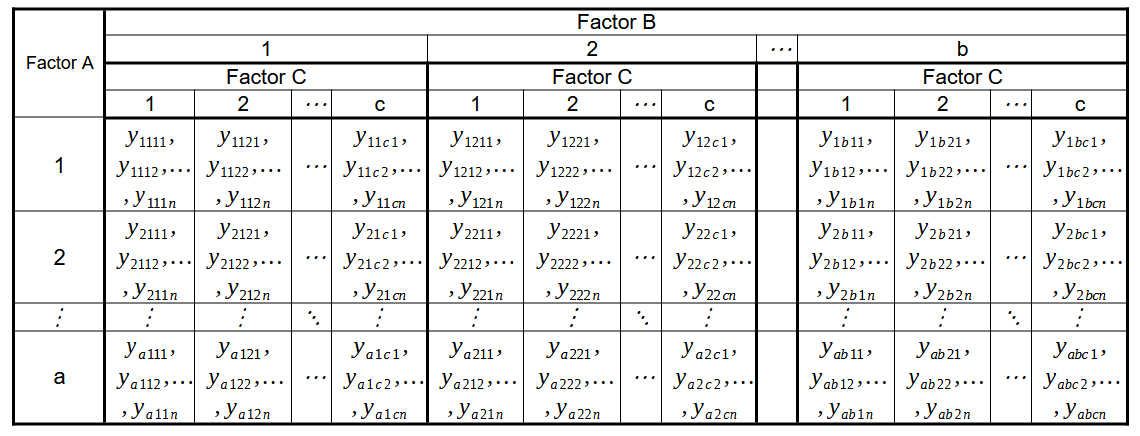
\includegraphics[width=0.90\linewidth]{img/factorial.png} 
	\caption{Disposición general para un diseño factorial con tres factores de efectos fijos.} 
	\label{fig:FactorialTres}
\end{figure}
\FloatBarrier

\textbf{El modelo para un diseño de tres factores es:}\\
	\begin{center}
	$y_{ijkl}=\mu + \tau_{i} + \beta_{j} + \gamma_{k} + (\tau \beta)_{ij} +(\tau \gamma)_{ik} + (\beta \gamma)_{jk} + (\tau \beta \gamma)_{ijk} + \epsilon_{ijkl} $

	$i = 1,2, \dots, a$, $j = 1,2, \dots, b$, $k = 1,2, \dots, c$  y $l = 1,2, \dots, n$
 \end{center}
 
Donde:
\begin{itemize}
	\item $\mu$ es la media general
	\item $\tau_{i}$ efecto del $i$-ésimo nivel del factor renglón $A$.
	\item $\beta_{j}$ efecto del $j$-ésimo nivel del factor columna $B$.
	\item $\gamma_{k} $ efecto del $k$-ésimo nivel del factor columna $C$.
	\item $(\tau \beta)_{ij} $ efecto de la interacción entre $\tau_{i}$  y  $\beta_{j}$ .
	\item $(\tau \gamma)_{ik}$ efecto de la interacción entre  $\tau_{i}$  y  $\gamma_{k}$ .
	\item $(\beta \gamma)_{jk}$ efecto de la interacción entre $\beta_{j}$ y  $\gamma_{k}$ .
	\item $(\tau \beta \gamma)_{ijk}$ efecto de la interacción entre $\tau_{i}$  , $\beta_{j}$ y $\gamma_{k}$ .
	\item $\epsilon_{ijkl}$ es el error aleatorio.
\end{itemize}


\textbf{Supuestos del modelo}\\
 $\epsilon_{ijkl} NI (0, \sigma^{2})$

\textbf{Hipótesis}\\
Para los factores
\begin{center}
	$H^{1}_{0} =\tau_{1} = \tau_{2} = \dots = \tau_{a} = 0$ vs $H^{1}_{1}$ : al menos una $\tau_{i} \neq 0$ , $i = 1,2, \dots, a$ \\
	$H^{2}_{0} =\beta_{1} = \beta_{2} = \dots = \beta_{b} = 0 $ vs $H^{2}_{1}$ : al menos una $\beta_{j} \neq 0$ , $j = 1,2, \dots,b$ \\
	$H^{3}_{0} =\gamma_{1} = \gamma_{2} = \dots = \gamma_{c} = 0 $ vs $H^{3}_{1}$ : al menos una $\gamma_{k} \neq 0$ , $k = 1,2, \dots,c$ \\
\end{center}

Para las interacciones 
\begin{center}
	$H^{4}_{0} : (\tau \beta)_{ij} = 0$ $ \forall i,j$ vs $H^{4}_{1}$ : al menos una $(\tau \beta)_{ij} \neq 0$ , $i = 1,2, \dots, a; j = 1,2, \dots,b$ \\
	$H^{5}_{0} : (\tau \gamma)_{ik} = 0$ $ \forall i,k$ vs $H^{5}_{1}$ : al menos una $(\tau \gamma)_{ik} \neq 0$ , $i = 1,2, \dots, a; k = 1,2, \dots,c$ \\
	$H^{6}_{0} : (\beta \gamma)_{jk} = 0$ $ \forall j,k$ vs $H^{6}_{1}$ : al menos una $(\beta \gamma)_{jk} \neq 0$ , $j = 1,2, \dots, b; k = 1,2, \dots, c$ \\
	$H^{7}_{0} : (\tau \beta \gamma)_{ijk} = 0$ $ \forall i,j,k$ vs $H^{7}_{1}$ : al menos una $(\tau \beta \gamma)_{ijk} \neq 0$ , $i = 1,2, \dots, a; j = 1,2, \dots, b; k = 1,2, \dots, c$ \\
\end{center}

\textbf{Suma de cuadrados}\\
Las fórmulas de cálculo para las sumas de cuadrados son:\\
$ SC_{total} = \sum_{i=1}^{a}  \sum_{j=1}^{b}  \sum_{k=1}^{c}  \sum_{l=1}^{n} y_{ijkl}^{2} - \frac{y_{....}^{2}}{abcn} $\\

$ SC_{A} = \sum_{i=1}^{a} \frac{y_{i...}^{2}}{bcn}  - \frac{y_{....}^{2}}{abcn} $\\

$ SC_{B} = \sum_{j=1}^{b} \frac{y_{.j..}^{2}}{acn}  - \frac{y_{....}^{2}}{abcn} $\\

$ SC_{C} = \sum_{k=1}^{c} \frac{y_{..k.}^{2}}{abn} - \frac{y_{....}^{2}}{abcn} $\\


\textbf{Las sumas de cuadrados para las interacciones son:}\\

$ SC_{AB} = \sum_{i=1}^{a} \sum_{j=1}^{b}  \frac{y_{ij..}^{2}}{cn}  - \frac{y_{....}^{2}}{abcn} - SC_{A} -SC_{B}  $\\

$ SC_{AC} = \sum_{i=1}^{a} \sum_{k=1}^{c}  \frac{y_{i.k.}^{2}}{bn}  - \frac{y_{....}^{2}}{abcn} - SC_{A} -SC_{C}  $\\

$ SC_{BC} = \sum_{j=1}^{b} \sum_{k=1}^{c}  \frac{y_{.jk.}^{2}}{an}  - \frac{y_{....}^{2}}{abcn} - SC_{C} -SC_{B}  $\\


$ SC_{ABC} =  \sum_{i=1}^{a}  \sum_{j=1}^{b}  \sum_{k=1}^{c}  \frac{y_{ijk.}^{2}}{n}  - \frac{y_{....}^{2}}{abcn} - SC_{A} -SC_{B} - SC_{C} -SC_{AB} -SC_{AC} -SC_{BC}  $\\


La suma de cuadrados del error puede encontrarse restando la suma de cuadrados de cada efecto principal e interacción de la suma de cuadrados total:\\

\begin{center}
	$ SC_{E} = SC_{T} -SC_{A} - SC_{B}-SC_{C} -SC_{AB} -SC_{AC} -SC_{BC} -SC_{ABC} $\\
\end{center}

O bien,
\begin{center}
	$ SC_{E} = SC_{T} - SC_{Sub(ABC)} $\\
\end{center}

Donde
\begin{center}
	$ SC_{Sub(ABC)} = \sum_{i=1}^{a}  \sum_{j=1}^{b}  \sum_{k=1}^{c} \frac{y_{ijk.}^{2}}{n} - \frac{y_{....}^{2}}{abcn}  $\\
\end{center}


\textbf{Estadísticos de prueba}\\
Para probar la significación la fuente de variabilidad $X$, se divide $CM_{X}$ por el  $CM_{E}$; de modo que los valores grandes de este cociente implican que los datos no apoyan la hipótesis nula correspondiente:
\begin{center}
	$ F^{X} = \frac{CM_{X}}{CM_{E}} \sim F_{x,abc(n-1)}  $\\
\end{center}


Donde $x$ representa los grados de libertad asociados a la fuente de variabilidad $X$.\\

\textbf{Región de rechazo}\\

Con un nivel de significación dado $\alpha$, la región de rechazo se encuentra en la cola superior de la distribución F correspondiente:

\begin{center}
	$ RR : F_{0}^{X} > F_{a;x,abc(n-1)} $\\
\end{center}

$ F_{0}^{X} $ es el valor de la estadística de prueba correspondiente.

\textbf{Valor p}\\

Se considera la fuente de variación $(X)$ con su correspondiente estadístico de prueba.

\begin{center}
	$ P_{X} =  P( F_{a;x,abc(n-1)} \geq F_{0}^{X} ) $\\
\end{center}


\begin{table}
	\centering
	\begin{tabular}{|c|c|c|c|c|c|}
		\hline
		\makecell{Fuente de \\ variación} & SC & g.l & CM & $F_{0}$ & Valor - p \\ % Encabezados de columna
		\hline
		A & $SC_{A}$ & $a-1$ & $\frac{SC_{A}}{a-1}$ &  $\frac{CM_{A}}{CM_{E}}$ & $P(F \geq F_{0}^{A} )$ \\
		\hline
		B & $SC_{B}$ & $b-1$ & $\frac{SC_{B}}{b-1}$ &  $\frac{CM_{B}}{CM_{E}}$ & $P(F \geq F_{0}^{B} )$ \\
		\hline
		C & $SC_{C}$ & $c-1$ & $\frac{SC_{C}}{c-1}$ &  $\frac{CM_{C}}{CM_{E}}$ & $P(F \geq F_{0}^{C} )$ \\
		\hline
		AB & $SC_{AB}$ & $(a-1)(b-1)$ & $\frac{SC_{AB}}{(a-1)(b-1)}$ &  $\frac{CM_{AB}}{CM_{E}}$ & $P(F \geq F_{0}^{AB} )$ \\
		\hline
		AC & $SC_{AC}$ & $(a-1)(c-1)$ & $\frac{SC_{AC}}{(a-1)(c-1)}$ &  $\frac{CM_{AC}}{CM_{E}}$ & $P(F \geq F_{0}^{AC} )$ \\
		\hline
		BC & $SC_{BC}$ & $(b-1)(c-1) $ & $\frac{SC_{BC}}{(b-1)(c-1)}$ &  $\frac{CM_{BC}}{CM_{E}}$ & $P(F \geq F_{0}^{BC} )$ \\
		\hline
		ABC & $SC_{ABC}$ & $(a-1)(b-1)(c-1)$ & $\frac{SC_{ABC}}{(a-1)(b-1)(c-1)}$ &  $\frac{CM_{ABC}}{CM_{E}}$ & $P(F \geq F_{0}^{ABC} )$ \\
		\hline
		Error & $SC_{E} $ & $abc(n-1)$ & $\frac{SC_{E}}{abc(n-1)}$ & & \\
		\hline
		Total & $SC_{T}$ & $abcn-1$ & & &  \\
		\hline
	\end{tabular}
	\caption{Tabla del ANOVA para el diseño factorial de tres factores con efectos fijos.}
\end{table}
\FloatBarrier

\subsubsection{Comparación múltiple de Tukey}

Si el ANOVA indica que hay diferencia en el nivel medio de los factores resulta de interés llevar a cabo comparaciones entre las medias individuales para determinar diferencias específicas. Existiendo interacción significativa, los efectos de los factores no son independientes.\\


Con la prueba de Tukey el nivel de significación global es exactamente  cuando los tamaños de las muestras son iguales y como máximo $\alpha$ cuando los tamaños de las muestras son desiguales. Este método también puede utilizarse para construir intervalos de confianza sobre las diferencias en todos los pares de medias. Para estos intervalos, el nivel de confianza simultáneo es del $(1-\alpha)100\%$ cuando los tamaños de las muestras son iguales y de al menos $(1-\alpha)100\%$  cuando los tamaños de las muestras son desiguales.\\
%%%Revisar acentos

$H_{0}:\mu_{i} = \mu_{j}$ vs $H_{1}:\mu_{i} \neq \mu_{j}$ para toda $i \neq j$\\

 $\mu_{i} \neq \mu_{j}$ si $| \bar{Y}_{i} -\bar{Y}_{j} | > q_{\alpha} (p,f) \: \sqrt{\frac{CM_{E}}{n}} = T_{\alpha}$ (tamaños de las muestras iguales).\\
 

La tabla V del apéndice en Montgomery (2017) contiene $q_{\alpha} (p,f)$, valor del punto porcentual $\alpha$ superior del estadístico del rango estudentizado $q=\frac{ \bar{Y}_{max} -\bar{Y}_{min}}{ \sqrt{\frac{CM_{E}}{n}}}$, donde $\bar{Y}_{max}$ y $\bar{Y}_{min}$ son las medias muestrales mayor y menor respectivamente de un grupo de $p$ medias muestrales, $f$ son los gl asociados con $CM_{E}$.\\
 
Intervalo de confianza del  $(1-\alpha)100\%$ para $\mu_{i} - \mu_{j}$:\\
 
\begin{center}
	$ \bar{Y}_{max} -\bar{Y}_{min} -  q_{\alpha} (p,f) \: \sqrt{\frac{CM_{E}}{n}} \leq \mu_{i} - \mu_{j} \leq \bar{Y}_{max} -\bar{Y}_{min} + q_{\alpha} (p,f) \: \sqrt{\frac{CM_{E}}{n}} $ \\
\end{center}

Para tamaños de muestras desiguales, en la prueba de hipótesis se utiliza:\\

\begin{center}
	$ T_{\alpha} = \frac{q_{\alpha} (p,f)}{\sqrt{2}} \sqrt{CM_{E} (\frac{1}{n_{i}} + \frac{1}{n_{j}})}  $ \\
\end{center}


Los intervalos de confianza para la diferencia de los pares de medias se determinan con:\\


\begin{center}
	$ \bar{Y}_{max} -\bar{Y}_{min} -  \frac{q_{\alpha} (p,f)}{\sqrt{2}} \sqrt{CM_{E} (\frac{1}{n_{i}} + \frac{1}{n_{j}})}  \leq \mu_{i} - \mu_{j} \leq \bar{Y}_{max} -\bar{Y}_{min} + \frac{q_{\alpha} (p,f)}{\sqrt{2}} \sqrt{CM_{E} (\frac{1}{n_{i}} + \frac{1}{n_{j}})}  $ \\
\end{center}

A la versión para tamaños de las muestras diferentes se llama el procedimiento de Tukey-Kramer.

	\newpage
	\section{Metodología}
En este trabajo se propone un método que permite evaluar la precisión de un modelo con la técnica de regresión lineal; y se basa en implementar diversos esquemas de remuestreos y estimar la precisión, a través de intervalos de confianza Bootstrap para el coeficiente de determinación $R^2$, del modelo de regresión entre los valores reales y predichos del modelo que se desea evaluar.\\

Se consideraron cuatro escenarios posibles con respecto al cumplimiento o no de los supuestos de normalidad y de varianza constante para un modelo a evaluar: NVC, NNVC, NVD y NNVD. Para estimar la distribución del coeficiente de determinación $R^2$, se implementan ocho esquemas de remuestreo: el Bootstrap Robusto Simple; el Wild Bootstrap robusto propuesto en \textcite{rana-2012} con los tres esquemas de remuestreo propuestos por\textcite{wu-1986}, y los dos esquemas propuestos por \textcite{wu-1986}; el Bootstrap de residuales balanceado y el Bootstrap pareado balanceado. Se proponen los intervalos percentiles y el BCa para estimar $R^2$ y para su cómputo se utilizan $B=1,000$ remuestras para cada uno de los esquemas Bootstrap.\\ 

Se realizó un estudio de simulación para comparar las eficiencias de los intervalos de confianza para los diferentes esquemas Bootstrap, tamaños de muestra y tipo de modelo; se simularon y evaluaron un total de 120,000 modelos, de los cuales 60,000 modelos fueron Exactos-Precisos (EP) y 60,000 fueron Exactos-Imprecisos (EI); para cada uno de los modelos se identificaron las $R^2$ de origen utilizadas para su simulación. Se simularon modelos de tamaños $n=10, 15, 20, 25, 30, 35$ para cada uno de los supuestos y tipo de modelo.\\  

Se consideraron tres criterios para determinar las eficiencias de los intervalos para cada esquema Bootstrap, el primer criterio determina la eficiencia como el porcentaje de las veces en que el intervalo contiene a la $R^2$ de origen para los modelos EP simulados; y viceversa, para los modelos IP la eficiencia se determinó como el porcentaje de las veces en que el intervalo de confianza no contiene a la $R^2$ de origen. El segundo criterio determina la eficiencia como el porcentaje de las veces en que ambos intervalos contienen de manera simultánea a la $R^2$ de origen para los modelos EP y de manera viceversa cuando ambos no la contienen para los modelos EI; y el tercer criterio determina la eficiencia como el porcentaje de las veces en que uno de los intervalos es más estrecho que el otro cuando ambos intervalos contienen simultáneamente la $R^2$ de origen para los modelos EP y de manera viceversa uno de los intervalos es más estrecho que el otro cuando ambos no la contienen simultáneamente para los modelos EI.\\

Se analizaron las eficiencias de los intervalos para cada tipo de supuesto a través de un ANOVA factorial para identificar diferencias significativas entre los tipos de intervalos, tipos de esquemas y tamaños de muestra; complementándolo con pruebas de Tukey. De acuerdo al análisis de los resultados se consideró una propuesta final para la evaluación de la precisión de un modelo, la cual se implementó en el lenguaje R \parencite{R-2024}; y se ilustra con dos modelos correspondientes a casos reales que se ajustaron a cada uno los diferentes escenarios.




\subsection{Una propuesta para evaluar la precisión de un modelo}

En esta propuesta para evaluar la precisión de un modelo se considera: el conocimiento del tipo de caso de esté ante los cuatro escenarios posibles bajo el cumplimiento de los supuestos de normalidad y/o varianza contante, los predichos $(z)$, los observados $(y)$ para generar muestras Bootstrap del coeficiente de determinación $R^{2}$. Se propone construir intervalos de confianza con el método Percentil y BCa a través de las muestras obtenidas, por ocho esquemas Bootstrap. \\ 

\subsubsection{Estimadores y esquemas Bootstrap}

Se debe considerar tres tipos de casos bajo el cumplimiento de los supuestos de normalidad y/o varianza contante:

\begin{description}
	\item[] Caso - 1 NVC
	\item[] Caso - 2 NNVC
	\item[] Caso - 3 NVD o NNVD
\end{description}


Es necesario construir los intervalos de confianza con los métodos: Percentil y BCa para la $R^{2}$. Dado el desconocimiento de la función de distribución del coeficiente de determinación, se propone el uso de los esquemas Bootstrap propuestos en \textcite{rana-2012} e implementados en \textcite{zacarias-2023}, al igual de los dos esquemas Bootstrap implementados en \textcite{balam-2012}. Dependiendo el caso a evaluar se utiliza los estimadores de mínimos cuadrados o el MM-estimador robusto.\\


\textit{Estimador de mínimos cuadrados para el Caso 1- NVC.}. En este caso se propone utilizar los estimadores al correr una regresión simple, junto a los residuales y los valores ajustados $\hat{y}$ obtenido por la regresión.\\


\textit{MM-estimador para el Caso 2- NNVC y  Caso - 3 NVD o NNVD}. En ambos casos se propone utilizar el MM-estimador con regresión robusta junto con los residuales robustos y los valores ajustados $\hat{y}$ robustos obtenidos por la regresión. Para el Caso 2- NNVC, los residuales robustos se utilizan sin ponderar y para el  Caso - 3 NVD o NNVD los residuales robustos se ponderarán.  \\



\textit{Bootstrap robusto y Bootstrap de Residuales Balanceados para todos los casos}. Para todos los casos se propone utilizar siete esquemas Bootstrap a los residuales dependiendo sus caso, los siguientes esquemas robustos: los tres de Wu (\textit{Algoritmo 3.5.1.1, Algoritmo 3.5.1.2 y Algoritmo 3.5.1.3}), los dos de Liu (\textit{Algoritmo 3.5.1.4 y Algoritmo 3.5.1.5}) y el Bootstrap simple (\textit{Algoritmo 3.4.7} y \textit{Algoritmo 3.4.2}). Adicionalmente, se propone implementar junto a los seis esquemas robustos, el Bootstrap de residuales balanceados (\textit{Algoritmo 3.4.5}). \\


\textit{Bootstrap Pareado Balanceado para todos los casos}. El Bootstrap Pareado Balanceado (\textit{Algoritmo 3.4.6}) al aplicar el remuestreo sobre una muestra pareada de las observaciones con su respectiva predicha y no depender de los estimadores al no utilizar los residuales, se implementa sin importar el tipo de caso, con los predichos $z$ y los observados $y$ del modelo a evaluar.\\

Este proceso que permite utilizar los esquemas Bootstrap dependiendo del caso del modelo se encuentra descrito en la Figura \ref{fig:AlgDifEsqBoots} e implementado en la función \textit{CalcularR2Bootstrap()} (Anexo C1).

 

\begin{figure}[ht!]
	\centering 
	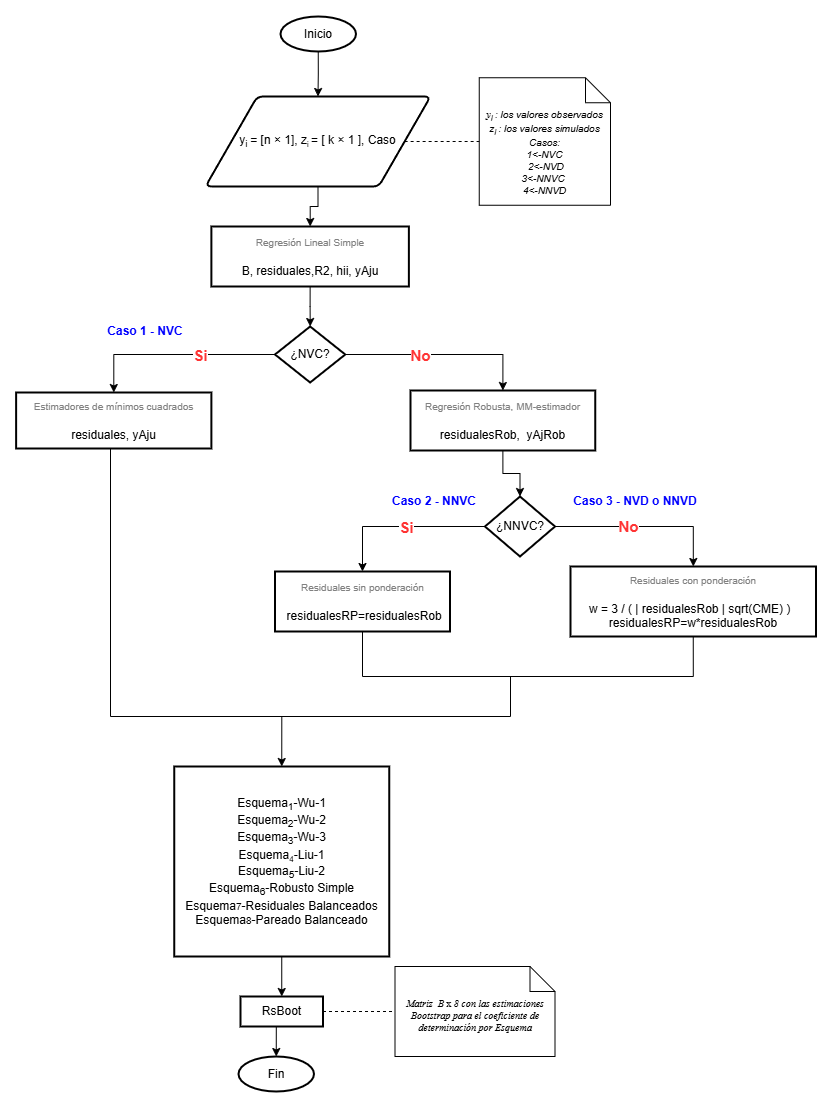
\includegraphics[width=0.7\linewidth]{img/metodologia_v7.png} 
	\caption{Diagrama de flujo para los diferentes esquemas Bootstrap.}
	\label{fig:AlgDifEsqBoots}
\end{figure}
\FloatBarrier

\subsubsection{Intervalos de confianza para la $R^{2}$}

Para evaluar la precisión del modelo se propone utilizar los intervalos de confianza Percentil y BCa para cada una de las muestras de $R^{2}s$ obtenidas en el procedimiento anterior por esquema Bootstrap. Debido a que las muestra Bootstrap de $R^{2}s$ ya se tiene, para el computo del ICB Percentil el \textit{Algoritmo 3.6.1} se comienza desde el paso 3. Y para el computó del ICB BCa se realiza el paso 1 del \textit{Algoritmo 3.6.2} en el cual se obtiene la estimación de la $R^{2}$ a partir de los datos originales del modelo, y se omiten los pasos 2 y 3 de dicho algoritmo ya que como en el caso anterior se cuenta con la muestra Bootstrap de $R^2 s$. La construcción de los ICB está implementada en la función \textit{ContruirIntervBoot()} (Anexo C2). \\



A continuación, se describe el algoritmo implementado en la función \textit{EvalPrecisionModel()} (Anexo C3) para evaluar la precisión de un modelo construyendo intervalos de confianza para cada esquema Bootstrap:\\


\textbf{Algoritmo 4.1.2.1 - Evaluación la Precisión de un Modelo}

\begin{enumerate}
	
	\item Calcular $e_i$ y $\hat{y}_{i}$ con los estimadores correspondientes a su caso (Caso - 1, Caso - 2 y Caso - 3).
	
	\item Llamar la función \textit{CalcularR2Bootstrap()} y aplicar el algoritmo con los esquemas Bootstrap para generar la matriz \( \mathbf{RsBoot} \) de orden \( b \times k \), donde:
	\begin{itemize}
		\item \( b \) es el número de remuestras generadas (\( \hat{R}^{2*}_{1}, \hat{R}^{2*}_{2}, \dots, \hat{R}^{2*}_{b} \)).
		\item \( k \) es el número de esquemas Bootstrap considerados (\( k = 8 \)).
	\end{itemize}
	
	\item Para cada columna \( k \) (\( k = 1, 2, \dots, 8 \)) en la matriz de remuestras \( RsBoot \):
	\begin{itemize}
		\item  Llamar a la función \textit{ContruirIntervBoot()} para construir el intervalo de confianza Percentil \( [LI_{P_k}, LS_{P_k}] \) utilizando el \textit{Algoritmo 3.6.1} modificado previamente.
		\item Llamar a la función \textit{ContruirIntervBoot()} para construir intervalo de confianza BCa \( [LI_{BCa_k}, LS_{BCa_k}] \) utilizando el \textit{Algoritmo 3.6.2} modificado previamente.
	\end{itemize}
\end{enumerate}





	 
\subsection{Estudio de simulación para la evaluación de la propuesta}

Para evaluar la eficiencia de los intervalos de confianza con los diferentes esquemas Bootstrap, se realizó un estudio de simulación donde se simularon modelos con la propuesta de \textcite{febles-2014} y las mejoras establecidas en \textcite{zacarias-2023}; considerando los siguientes factores: Precisión (EP, EI), Supuestos (NVC, NVD, NNVC, NNVD) y tamaño de muestra $(10, 15, 20, 25, 30, 35)$.\\


\subsubsection{Simulación de los modelos}
Para la simulación de los modelos se utilizaron los simuladores $ModNVC()$, $ModNNVC()$, $ModNNVD()$ y$ ModNVD()$ descritos en la sección 3.7. Para este trabajo se simularon modelos de tipo EP y EI, por lo que se consideraron valores \textit{a priori} fijos para el intercepto y la pendiente con b0=0 y b1=1; lo cual implicó que para el uso de los simuladores solo se tuviera que especificar tres argumentos: n, R2 y muz.\\

Los modelos se simularon para tamaños de muestra $n=10, 15, 20, 25, 30, 35$; para los valores hipotéticos de $R^2$, se seleccionaron números aleatorios en el intervalo (0.8, 0.99) para los modelos EP y números aleatorios en el intervalo (0.1, 0.3) para los modelos EI, en ambos casos los números se redondearon a cuatro decimales. Para la especificación de muz se consideraron número aleatorios en el intervalo (5,100).\\
 

\subsubsection{Generación y respaldo de los modelos simulados}

Para la simulación y el respaldo de todos los modelos utilizados para evaluar la propuesta de este trabajo, se desarrolló la función $SimMod(N,n,r,TipoPres,TipoSupues)$; la cual tiene como argumentos el número de modelos que se desean simular (N); el tamaño de la muestra (n); el número de réplicas para cada modelo (r);  la precisión deseada (TipoPres; 1: Preciso, 2:Impreciso); y tipo de supuesto que debe cumplir el modelo simulado (TipoSupues; 1:NVC, 2:NVD, 3:NNVC, 4:NNVD). Para todos los tipos de modelos simulados se consideraron $r=5$ réplicas para $N=500$ modelos; de tal forma que, para un tamaño de muestra fijo, un tipo de precisión fijo y un tipo de supuesto fijo se simularon 2,500 modelos; por lo que en total se simularon y respaldaron $120,000$ modelos $(2500 \times 6 \times 2 \times 4)$, la mitad fueron modelos EP y la otra mitad modelos EI.
La función $SimEP()$ ejecuta para cada réplica, el simulador correspondiente ($ModNVC()$, $ModNVD()$,$ ModNNVC()$,$ ModNNVD()$) $N$ veces para la simulación de los modelos correspondientes a cada tipo de supuesto. Al final, la función $SimMod()$ guarda los modelos simulados por cada tamaño de muestra, tipo de precisión y tipo de supuesto en una matriz de tamaño $rn \times 2N$ y también guarda en otra matriz de tamaño $r \times N$ a las $R^2$ de origen correspondientes a cada uno de los modelos simulados, en total se respaldaron 48 matrices que contienen los 120,000 modelos y 48 matrices que contienen las $R^2$ de origen correspondiente a cada modelo simulado. Las matrices se utilizaron para determinar las eficiencias de los métodos Bootstrap propuestos para la medición de la precisión de un modelo. Para más detalle sobre la función $SimMod()$ ver Anexo C5.\\

En el Anexo C6, se muestran las ejecuciones realizadas a la función $SimMod()$ para la simulación y respaldo de los 120,000 modelos utilizados. \\


\subsubsection{Evaluación de la precisión de los modelos}

Después de simular los modelos hipotéticos EP e EI con los cuatro supuestos, se construyó la función $ProcesarModels()$ (Anexo C4) que utiliza la función $EvalPrecisionModel()$ para evaluar la precisión, donde para la primera función $ProcesarModels$, recibe los siguientes argumentos: $"archivos \_ encontrados"$ que representa dos archivos: la matriz de $rn \times 2N$ con los modelos y la matriz de $r \times N$ con las $R^2$ de origen respectivas; $"caso"$ indica el tipo de escenario de los modelos, con 1 como Normalidad- Homocedasticidad, 2 como Normalidad-Heterocedasticidad, 3 como No normalidad-Homocedasticidad y 4 como No normalidad-Heterocedasticidad; $"replicas"$ como el número de replicas del estudio; $"nivConfianza"$ como el nivel de confianza para el I.C. para la $R^2$; $"N"$ como el tamaño de muestra de los modelos; $"MODELO"$ para indicar si es preciso o impreciso y $"CASO"$ como una etiqueta del tipo de supuesto($"NVC","NVD","NNVC","NNVD"$).\\


La función al procesar ambas matrices (modelos y sus $R^2$s de origen) por replica, recupera uno por uno los modelos y se le aplica a la función $EvalPrecisionModel()$ que implementa el \textit{Algoritmo 4.1.2.1} con $B=1,000$ remuestras Bootstrap por cada uno de los ocho tipos de remuestreos y calcula los I.C., el cual recibe los parámetros de $"data"$ como el vector $ z \times y $ con los predichos y las observaciones respectivamente del modelo;  $"alpha"$ como el nivel de significancia; $" nivConfianza" $, el nivel de confianza y el $"caso"$, que retorna una lista de ocho matrices de tamaño $2 \times 2$, donde cada fila de matriz contiene los ICB Percentil e ICB BCa para el coeficiente de determinación calculado por cada esquema para el modelo.\\


\subsubsection{Determinación de la eficiencia de los intervalos y esquemas}

Al obtener la lista con los I.C. para la $R^2$ del modelo, estos se procesan por esquema y  se realizan las evaluaciones para determinar las eficiencias, pero antes, deber cumplir el criterio de que los intervalos con el esquema hayan sido calculados, es decir, son valores válidos, para considerarlo un modelo eficaz con el esquema. La eficiencia se determinó como el porcentaje de veces que los intervalos contienen a la \( R^2 \) de origen empleada para simular el modelo. Adicionalmente, para evaluar cuál de los dos intervalos es más eficaz, se consideraron dos escenarios: si solo uno de los intervalos logró contener la \( R^2 \), se consideró ganador por defecto y la eficiencia se calculó como el porcentaje de veces en que solo uno de los intervalos incluyó la \( R^2 \); en caso de empate, es decir, cuando ambos intervalos contuvieron la \( R^2 \), se consideró más eficiente el intervalo con menor amplitud, ya que proporciona una estimación más precisa. La eficiencia en este caso se calculó como el porcentaje de veces que ambos intervalos incluyeron la \( R^2 \), pero uno de ellos fue más estrecho.\\

La eficiencia de los esquema Bootstrap, se determinó como el porcentaje de veces que logra que ambos intervalos contengan a la \( R^2 \) de origen con respecto a los modelos evaluados.\\

Los resultado de las eficiencias se respaldan por supuesto, tipo de modelo y tamaño de muestra, y sus réplicas con dos tablas: la primera tabla para la eficiencia de los intervalos se guarda el número de réplica, el identificador del esquema utilizado, el número de modelos dados por la réplica, el número de modelos eficaces en la réplica que cumplieron la condición de construir ambos intervalos con valores válidos, la frecuencia de que el I.C Percentil es eficiente, la frecuencia de que el I.C BCa es eficiente, la frecuencia en la que el I.C Percentil fue el ganador por defecto, la frecuencia en la que el I.C BCa fue el ganador por defecto, la frecuencia en la que el I.C. Percentil fue mejor que el I.C. BCa cuando ambos fueron ganadores y la frecuencia en la que el I.C. BCa fue mejor que el I.C. Percentil cuando ambos fueron ganadores. La segunda tabla, corresponde a la eficiencia de los esquemas por réplica determinado por el número de veces en la que el esquema logró hacer que sus ICB contuvieran a la \( R^2 \) de origen (Ver Anexo C4).\\

En total se construyeron 96 tablas para las eficiencias, de las cuales 48 fueron para modelos EP y 48 para modelos EI. Para resumir los resultados de las tablas se construyeron 8 nuevas tablas con las eficiencias promedios para cada tipo de modelo, donde para cada supuesto se construyó una tabla de eficiencias promedios para los ICB, por tamaño de muestra y esquema de remuestreo y otra para las eficiencias promedio de los esquemas por tamaño de muestra.\\

Finalmente, se construyó por cada tipo de modelo una tabla que resume la eficiencia promedio por cada supuesto y esquemas sin importar el tamaño de la muestra.\\


\subsection{Análisis estadísticos}
Para cada supuesto (NVC, NNVC, NVD, NNVD) se utilizó ANOVA en un arreglo factorial de tres factores seguido de la comparación múltiple de Tukey \parencite{montgomery-2017}, para determinar el comportamiento de la eficiencia de dos ICB en la evaluación de la precisión, bajo ocho esquemas de remuestreo, seis tamaños de muestra y dos tipos de modelo. Cabe señalar que, en cuatro de los ocho análisis de varianza realizados se eliminaron valores atípicos para el logro del cumplimiento de los supuestos del ANOVA.
Las pruebas estadísticas se consideraron significativas cuando el $pvalor<0.05$  y se utilizó el paquete estadístico STATGRAPHICS Centurion 19 \parencite{statgraphics-2024} .





	\newpage
	\section{Resultados}
En esta sección se presentan los resultados correspondientes a las eficacias de los intervalos de confianza, bajo los esquemas Bootstrap con los estimadores para la evaluación de la precisión de modelos EP y EI, cuando cumplen los supuestos de normalidad e igualdad de varianzas, y cuando no se cumplan los supuestos de normalidad y/o igualdad de varianzas.
\vspace{.5cm}

Al igual que los resultados correspondientes a las eficacias de los esquemas Bootstrap con los estimadores en la construcción de ICB que contienen al coeficiente de determinación en modelos EP y EI, cuando cumplen los supuestos de normalidad e igualdad de varianzas, y no se cumplan los supuestos de normalidad y/o igualdad de varianzas.



\subsection{Eficiencia de los intervalos Bootstrap para el caso EP-NVC}
Con base en el promedio general (Figura \ref{fig:EP_NVC_Boots}) para: Eficiencia del ICB Percentil (Efic Int Boot Perc) y Eficiencia en ICB BCa (Efic Int Boot Bca) el mejor esquema resultó Liu2, 0.9569 y 0.9586 respectivamente;
Eficiencia del ICB Percentil cuando solo él lo contiene a la $R^{2}$ y Eficiencia del ICB BCa cuando solo él contiene a la $R^{2}$ el mejor esquema es Liu1, 0.7354 y 0.7366 respectivamente;
la Eficiencia de ICB Percentil cuando gana en el empate a ICB BCa (Efic Boot Perc gana empate), el mejor esquema es Wu1 $(0.8989)$ y la Eficiencia ICB BCa cuando gana el empate al ICB Percentil (Efic Boot Bca gana empate), el mejor esquema es Wu3 $(0.4304)$.
\vspace{.5cm}

%Poner el contexto
Sin considerar el tamaño de la muestra, para el caso EP-NVC los ICB mejores en promedio general (Figura \ref{fig:EP_NVC_Boots}) son: el ICB Percentil con $0.8081$ ante la Eficiencia en ICB BCa; la Eficiencia del ICB Bca cuando solo él contiene a la $R^{2}$ $(0.1516)$ y la Eficiencia de ICB Percentil cuando gana en el empate al ICB Bca con $0.7047$.

\begin{figure}[H] 
	\centering 
	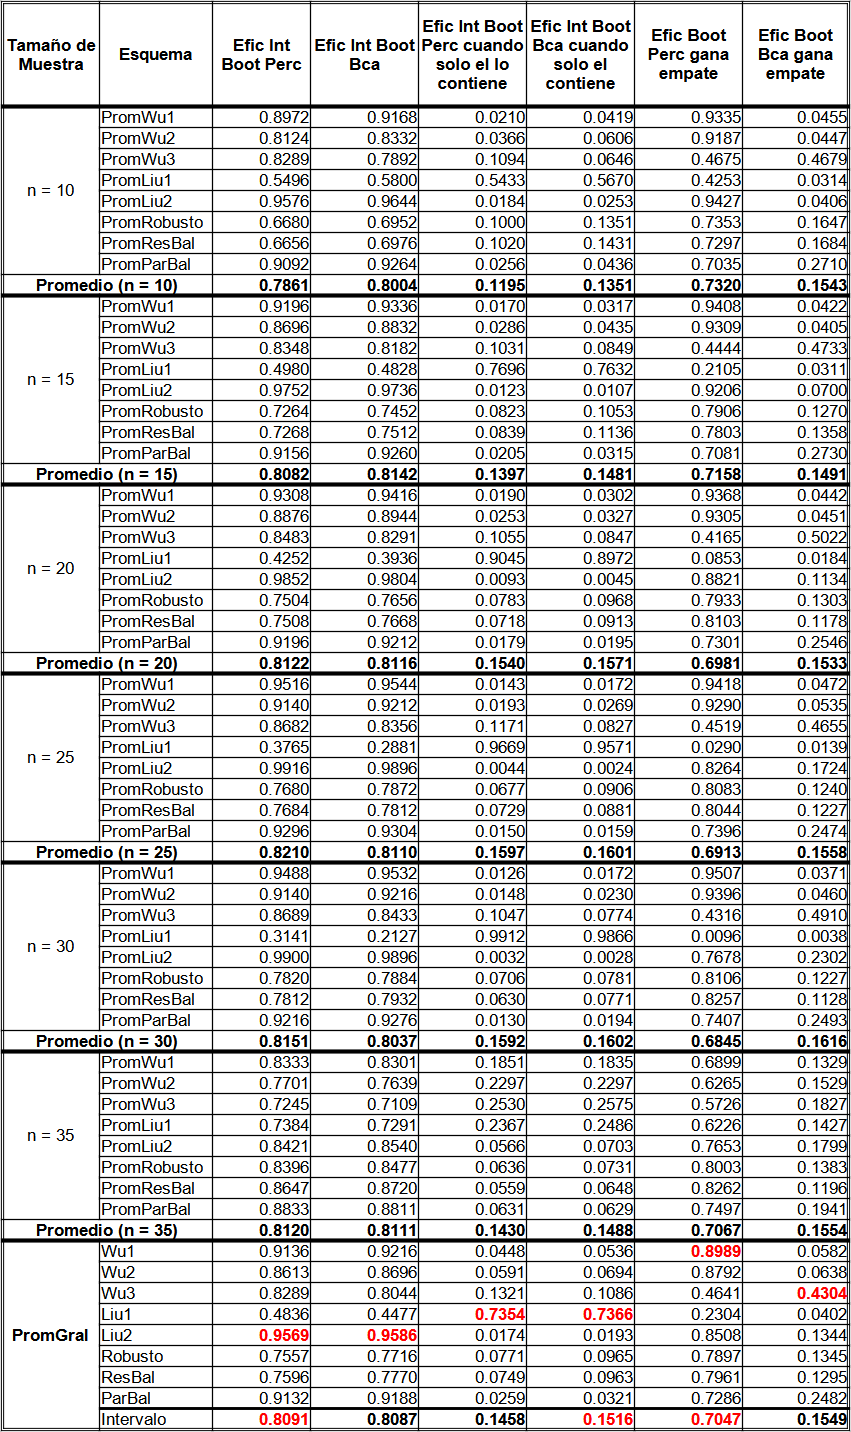
\includegraphics[width=0.55\linewidth]{img/EP_NVC_Efic_Boots.png} 
	\caption{Eficiencia promedio de los intervalos Bootstrap por tamaño de muestra y esquema de remuestreos para el caso EP-NVC.} 
	\label{fig:EP_NVC_Boots}
\end{figure}

\FloatBarrier

\subsubsection{Eficiencia de los esquemas para el caso EP-NVC}
Con base en el promedio de eficiencia por tamaño de muestra (Figura 4) y un nivel de confianza mayor o igual a 0.95: con tamaño de muestra 10 ningún esquema cumplió la condición, sin embargo con Liu2 se obtuvo 0.94, y con los tamaños de muestra 15, 20, 25, 30 y 35 el mejor fue es el esquema Lui2.
\vspace{.5cm}

Sin considerar el tamaño de la muestra, para el caso EP-NVC el mejor promedio general (Figura 4) en eficiencia de esquema es Liu2 (0.9737).


\begin{figure}[H] 
	\centering 
	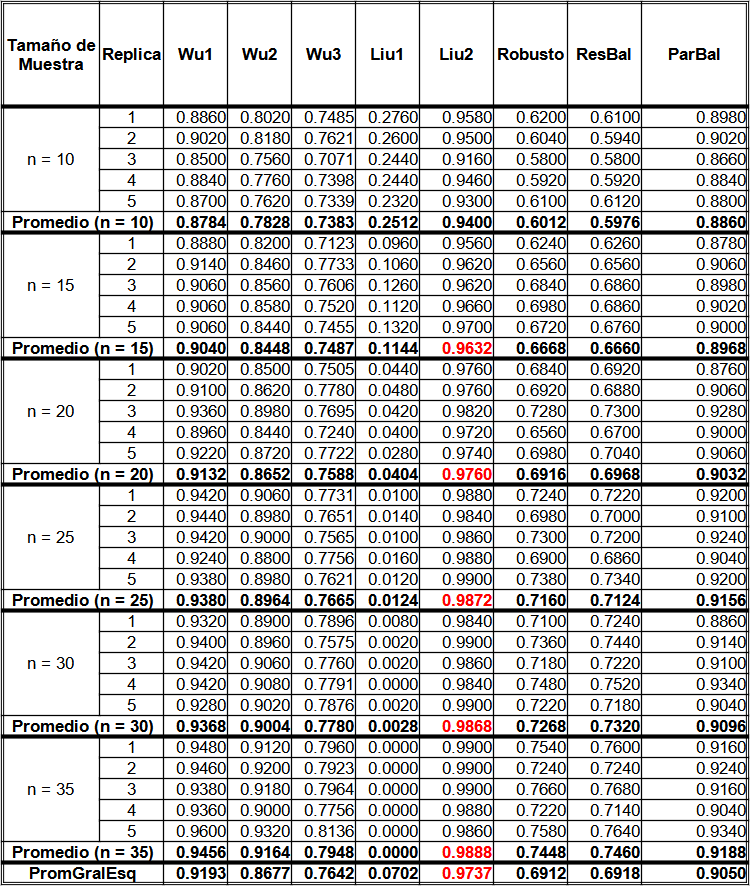
\includegraphics[width=0.70\linewidth]{img/EP_NVC_Efic_Esq.png} 
	\caption{Eficiencia promedio de los esquemas por tamaño de muestra y esquema de remuestreos para el caso EP-NVC.} 
	\label{fig:EP_NVC_Esq}
\end{figure}

\FloatBarrier

%%%%%%%%%%%%%%%%%%%%%%%%%%%%%%%%%%%%%%%%%%%
\subsubsection{Eficiencia de los intervalos Bootstrap para el caso EP-NNVC}
Con base en el promedio general (Figura 5) para: Eficiencia del ICB Percentil (Efic Int Boot Perc) y Eficiencia en ICB BCa (Efic Int Boot Bca) el mejor esquema resulto Liu2, 0.9893 y 0.9870 respectivamente;
Eficiencia del ICB Percentil cuando solo el lo contiene a la $R^{2}$ y Eficiencia del ICB BCa cuando solo el contiene a la $R^{2}$ el mejor esquema es Liu1, 0.6381 y 0.6549 respectivamente; 
la Eficiencia de ICB Percentil cuando gana en el empate a ICB BCa (Efic Boot Perc gana empate), el mejor esquema es Wu2 $(0.9026)$ y la Eficiencia ICB BCa cuando gana el empate al ICB Percentil (Efic Boot Bca gana empate), el mejor esquema es Wu3 $(0.8147)$.
\vspace{.5cm}


%Poner el contexto
Sin considerar el tamaño de la muestra, para el caso EP-NNVC los ICB mejores en promedio general  (Figura 5) son: Eficiencia del ICB BCa (Efic Int Boot Bca) con $0.8653$ ante la Eficiencia en ICB Percentil (Efic Int Boot Perc); la Eficiencia del ICB BCa cuando solo el contiene a la $R^{2}$ $(0.1117)$ y la Eficiencia de ICB Percentil cuando gana en el empate al ICB BCa (Efic Boot Perc gana empate) con $0.6697$.



\begin{figure}[ht] 
	\centering 
	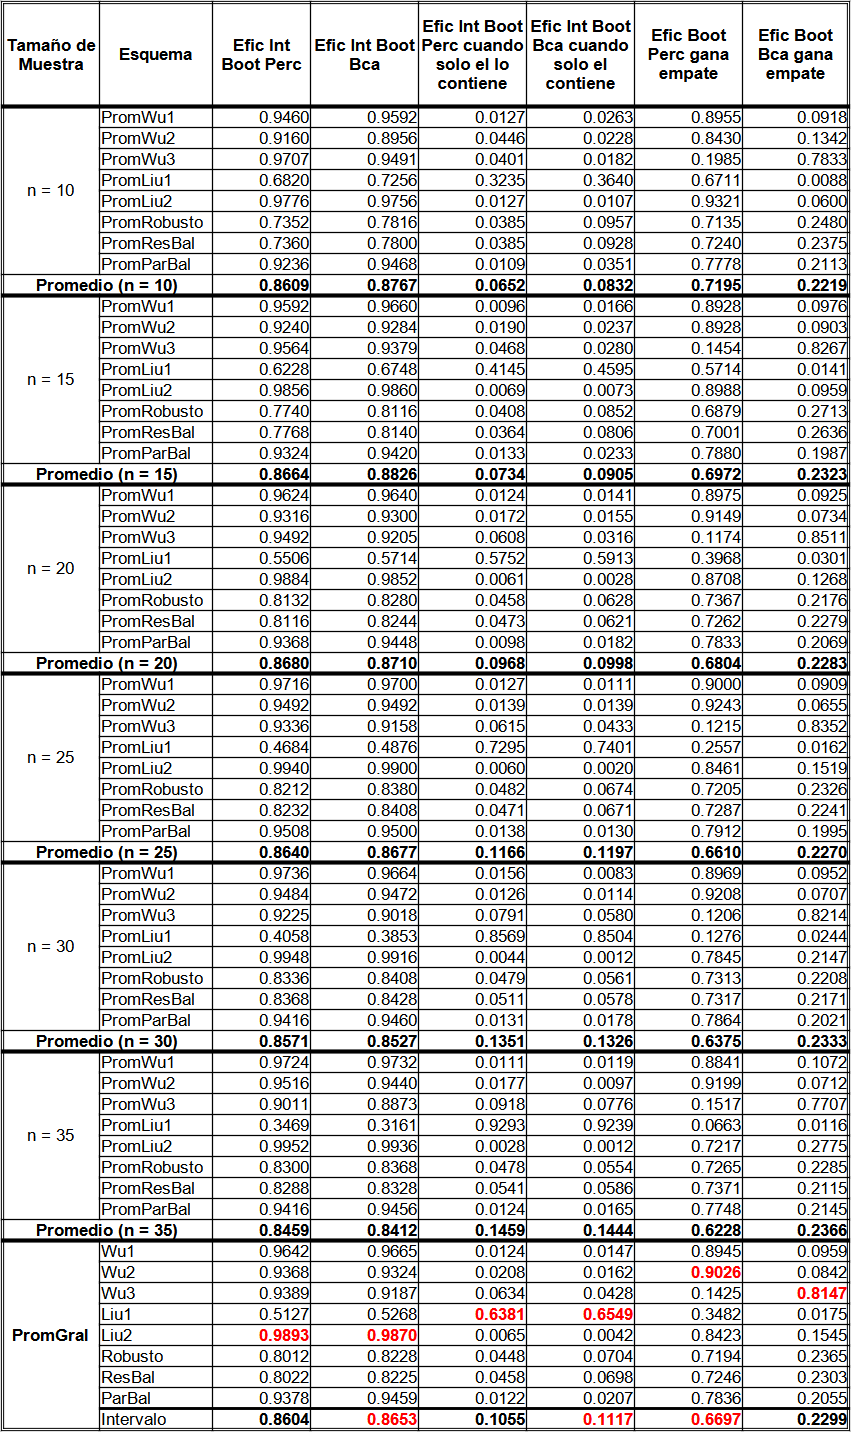
\includegraphics[width=0.55\linewidth]{img/EP_NNVC_Efic_Boots.png} 
	\caption{Eficiencia promedio de los intervalos Bootstrap por tamaño de muestra y esquema de remuestreos para el caso EP-NNVC.} 
	\label{fig:EP_NNVC_Boots}
\end{figure}
\FloatBarrier


\subsubsection{Eficiencia de los esquemas para el caso EP-NNVC}
Con base en el promedio de eficiencia por tamaño de muestra (Figura 6) y un nivel de confianza mayor o igual a 0.95: con tamaño de muestra 10 el mejor fue el esquema Liu2 (0.9651), seguido por Wu1 (0.9340) y con los tamaños de muestra 15, 20, 25, 30 y 35 los mejores esquemas son Liu2 y Wu1.
\vspace{.5cm}


Sin considerar el tamaño de la muestra, para el caso EP-NNVC los mejores promedio generales (Figura 6) en eficiencia son los esquema Liu2 y Wu1.


\begin{figure}[ht] 
	\centering 
	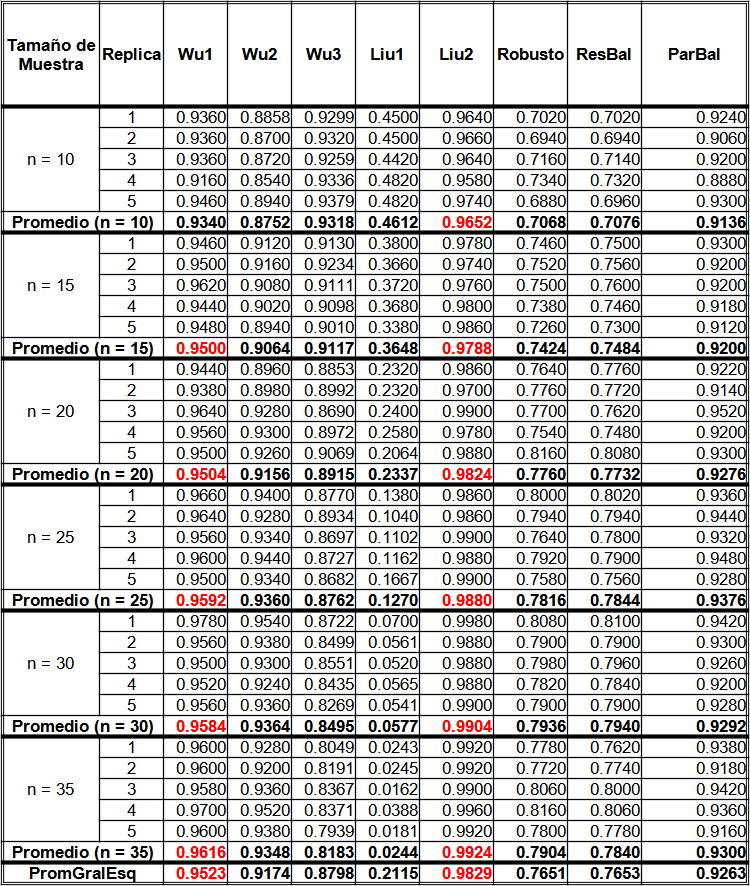
\includegraphics[width=0.70\linewidth]{img/EP_NNVC_Efic_Esq.png} 
	\caption{Eficiencia promedio de los esquemas por tamaño de muestra y esquema de remuestreos para el caso EP-NNVC.} 
	\label{fig:EP_NNVC_Esq}
\end{figure}
\FloatBarrier


%%%%%%%%%%%%%%%%%%%%%%%%%%%%%%%%%%%%%%%%%%%%%%%%

\subsubsection{Eficiencia de los intervalos Bootstrap para el caso EP-NVD}
Con base en el promedio general (Figura 7) para: Eficiencia del ICB Percentil (Efic Int Boot Perc) y Eficiencia en ICB BCa (Efic Int Boot Bca) el mejor esquema resulto Liu2, 0.9775 y 0.9760 respectivamente; Eficiencia del ICB Percentil cuando solo el lo contiene a la $R^{2}$ y Eficiencia del ICB BCa cuando solo el contiene a la $R^{2}$ el mejor esquema es Liu1, 0.5042 y 0.4677 respectivamente; 
la Eficiencia de ICB Percentil cuando gana en el empate a ICB BCa (Efic Boot Perc gana empate), el mejor esquema es Pareado Balanceado (ParBal) con 0.8230 y la Eficiencia ICB BCa cuando gana el empate al ICB Percentil, el mejor esquema es Wu3 $(0.5159)$.
\vspace{.5cm}


Sin considerar el tamaño de la muestra, para el caso EP-NVD los ICB mejores en promedio general (Figura 7) son: Eficiencia del ICB BCa (Efic Int Boot Bca) con $0.8299$ ante la Eficiencia en ICB Percentil (Efic Int Boot Perc); la Eficiencia del ICB Percentil cuando solo el contiene a la $R^{2}$ $(0.1049)$ y la Eficiencia de ICB BCa cuando gana en el empate al ICB Percentil (Efic Boot Bca gana empate) con $0.2942$.


\begin{figure}[ht] 
	\centering 
	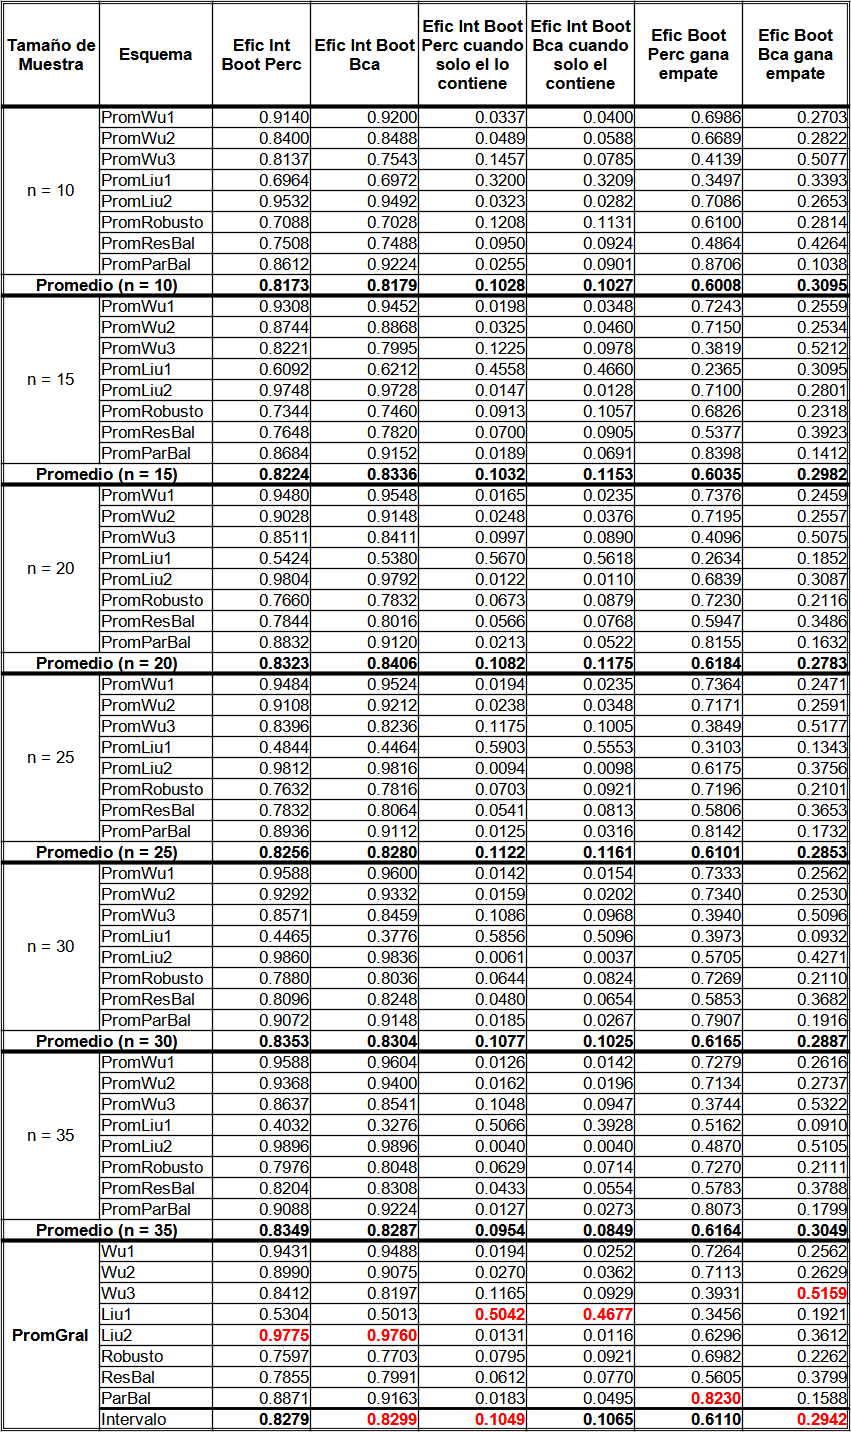
\includegraphics[width=0.55\linewidth]{img/EP_NVD_Efic_Boots.png} 
	\caption{Eficiencia promedio de los intervalos Bootstrap por tamaño de muestra y esquema de remuestreos para el caso EP-NVD.} 
	\label{fig:EP_NVD_Boots}
\end{figure}
\FloatBarrier

\subsubsection{Eficiencia de los esquemas para el caso EP-NVD}
Con base en el promedio de eficiencia por tamaño de muestra (Figura 8) y un nivel de confianza mayor o igual a 0.95: con tamaño de muestra 10 ningún esquema cumplió la condición, sin embargo con Liu2 se obtuvo 0.9224 y con los tamaños de muestra 15, 20, 25, 30 y 35 el mejor fue el esquema Lui2.
\vspace{.5cm}

Sin considerar el tamaño de la muestra, para el caso EP-NVD el mejor promedio general (Figura 8) en eficiencia de esquema es Liu2 (0.9648).


\begin{figure}[ht] 
	\centering 
	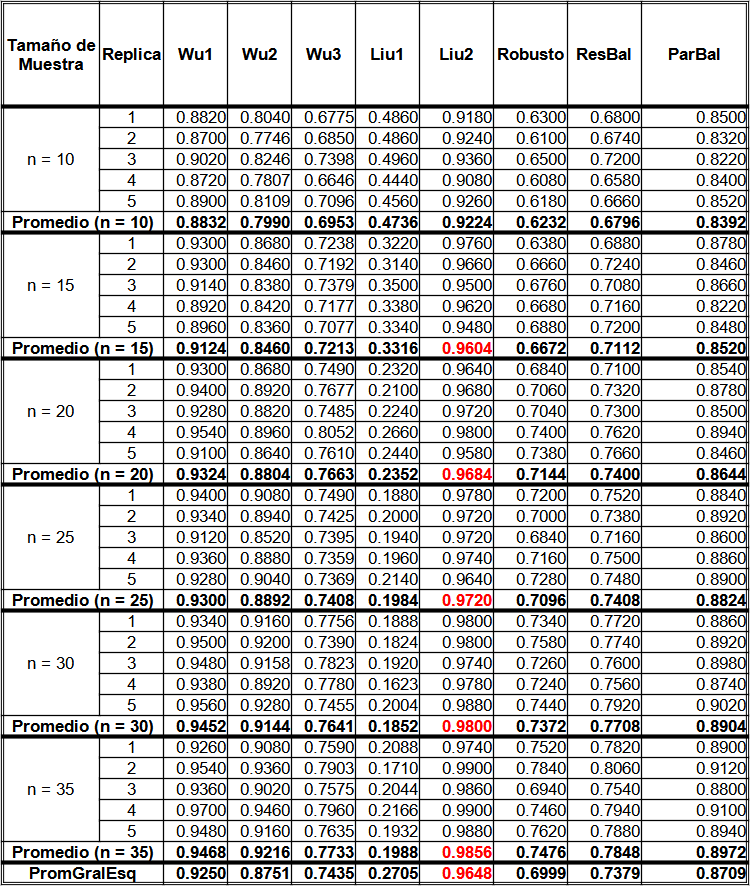
\includegraphics[width=0.70\linewidth]{img/EP_NVD_Efic_Esq.png} 
	\caption{Eficiencia promedio de los esquemas por tamaño de muestra y esquema de remuestreos para el caso EP-NVD.} 
	\label{fig:EP_NVD_Esq}
\end{figure}
\FloatBarrier


%%%%%%%%%%%%%%%%%%%%%%%%%%%%%%%%%

\subsubsection{Eficiencia de los intervalos Bootstrap para el caso EP-NNVD}
Con base en el promedio general (Figura 9) para: Eficiencia del ICB Percentil (Efic Int Boot Perc) el mejor esquema resulto Liu2 (0.9171); 
Eficiencia en ICB BCa (Efic Int Boot Bca) el mejor esquema resulto Pareado Balanceado (ParBal) con 0.9162;
 Eficiencia del ICB Percentil cuando solo el lo contiene a la $R^{2}$ y Eficiencia del ICB BCa cuando solo el contiene a la $R^{2}$ el mejor esquema resulto Wu3, 0.3156 y 0.2458 respectivamente;
 la Eficiencia de ICB Percentil cuando gana en el empate a ICB BCa (Efic Boot Perc gana empate), el mejor esquema es ParBal (0.7930) y la Eficiencia ICB BCa cuando gana el empate al ICB Percentil (Efic Boot Bca gana empate), el mejor esquema es de Residuales Balanceados (ResBal) con 0.8630.
\vspace{.5cm}


Sin considerar el tamaño de la muestra, para el caso EP-NNVD los ICB mejores en promedio general (Figura 9) son: Eficiencia del ICB Percentil (Efic Int Boot Perc) con $0.8186$ ante la Eficiencia en ICB BCa (Efic Int Boot Bca); la Eficiencia del ICB Percentil cuando solo el contiene a la $R^{2}$ $(0.1119)$ y la Eficiencia de ICB BCa cuando gana en el empate al ICB Perc (Efic Boot Bca gana empate) con $0.6286$.


\begin{figure}[ht] 
	\centering 
	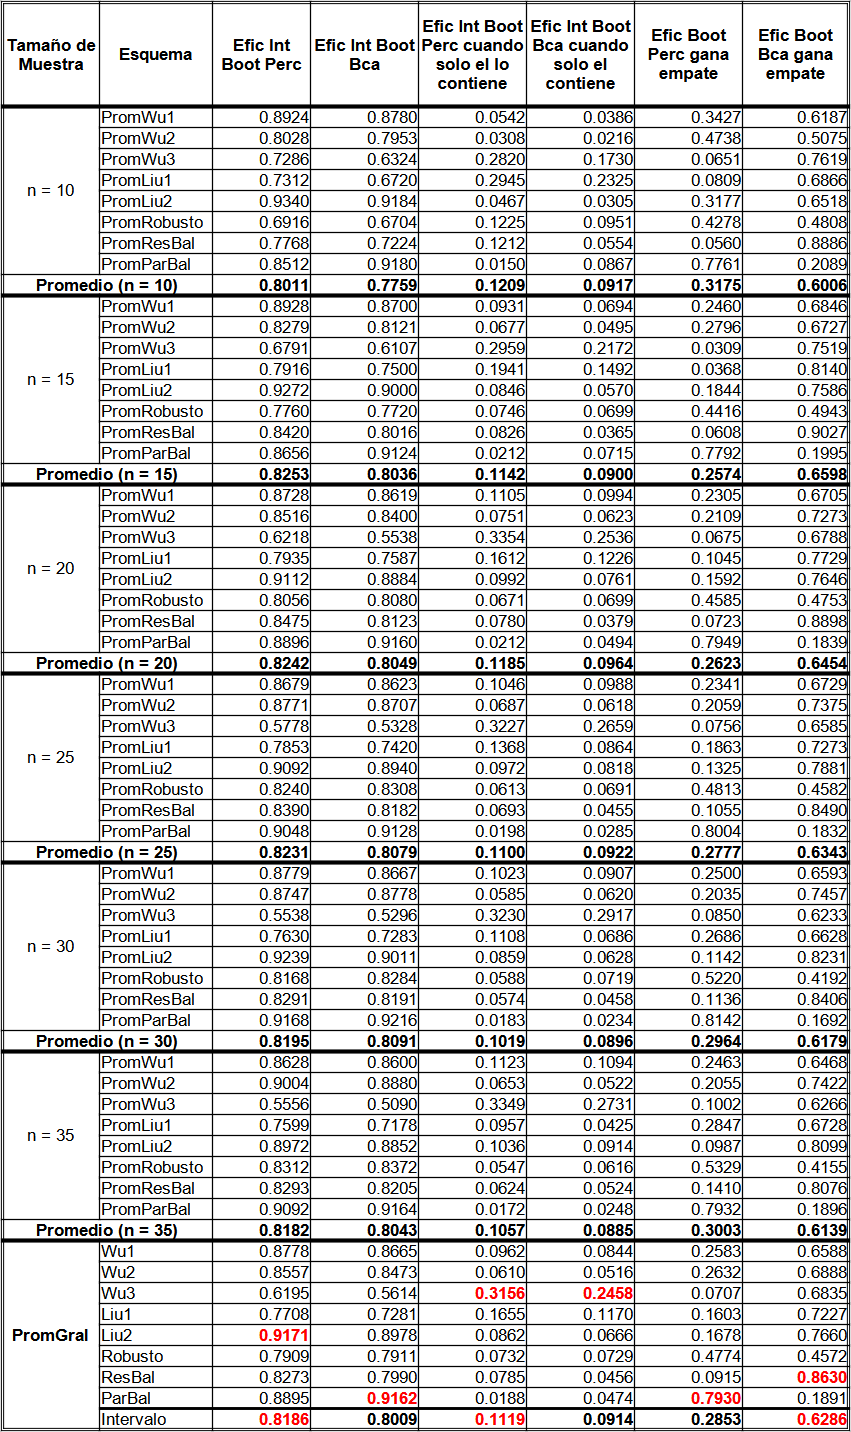
\includegraphics[width=0.55\linewidth]{img/EP_NNVD_Efic_Boots.png} 
	\caption{Eficiencia promedio de los intervalos Bootstrap por tamaño de muestra y esquema de remuestreos para el caso EP-NNVD.} 
	\label{fig:EP_NNVD_Boots}
\end{figure}
\FloatBarrier

\subsubsection{Eficiencia de los esquemas para el caso EP-NNVD}
Con base en el promedio de eficiencia por tamaño de muestra (Figura 10) y un nivel de confianza mayor o igual de 0.90: solo con el tamaño de muestra 30 se cumple la condición bajo el esquema Pareado Balanceado (ParBal) con 0.9. Ahora sin considerar el criterio anterior, el mejor esquema para: n=10 es Liu2 (0.8904) y Wu1(0.8440), n=15 es Liu2 (0.8488) y ParBal (0.8472), n=20 es ParBal (0.8708) y Liu2 (0.8207), n=25 es ParBal (0.8868) y Liu2 (0.8207), n=30 es ParBal (0.9) y Liu2 (0.8447) y en n=35 es ParBal (0.8936) y Wu2 (0.8415).  
\vspace{.5cm}


Sin considerar el tamaño de la muestra, para el caso EP-NNVD los mejores promedios generales (Figura 10) en eficiencia de esquema son ParBal (0.8728) y Liu2 (0.8383).


\begin{figure}[ht] 
	\centering 
	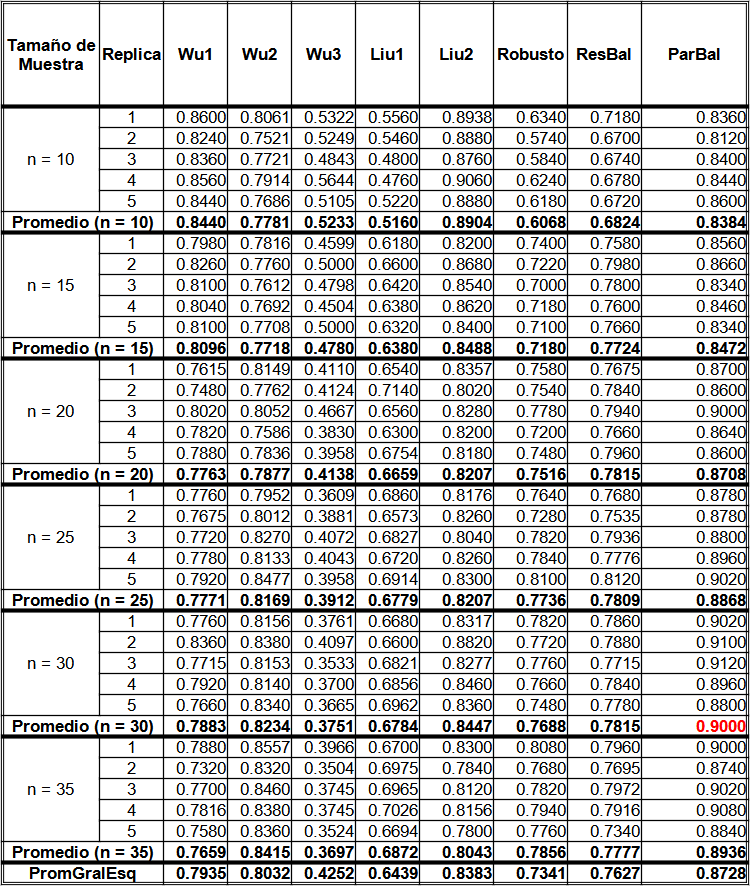
\includegraphics[width=0.70\linewidth]{img/EP_NNVD_Efic_Esq.png} 
	\caption{Eficiencia promedio de los esquemas por tamaño de muestra y esquema de remuestreos para el caso EP-NNVD.} 
	\label{fig:EP_NNVD_Esq}
\end{figure}
\FloatBarrier

%%Tipo de intervalo y esquema para evaluar la precision. 8 recomendaciones

%%%%%%%%%%%%%%%%%%%

\subsubsection{Promedio de supuestos para el caso EP}
Dados los modelos de tipo EP para los casos: Normalidad - Varianza Constante (NVC), No normalidad - Varianza Constante (NNVC), Normalidad - Varianza Distinta (NVD) y  No normalidad - Varianza Distinta (NNVD), con base en los promedios generales (Figura 11), se sugiere el uso de 




\begin{figure}[ht] 
	\centering 
	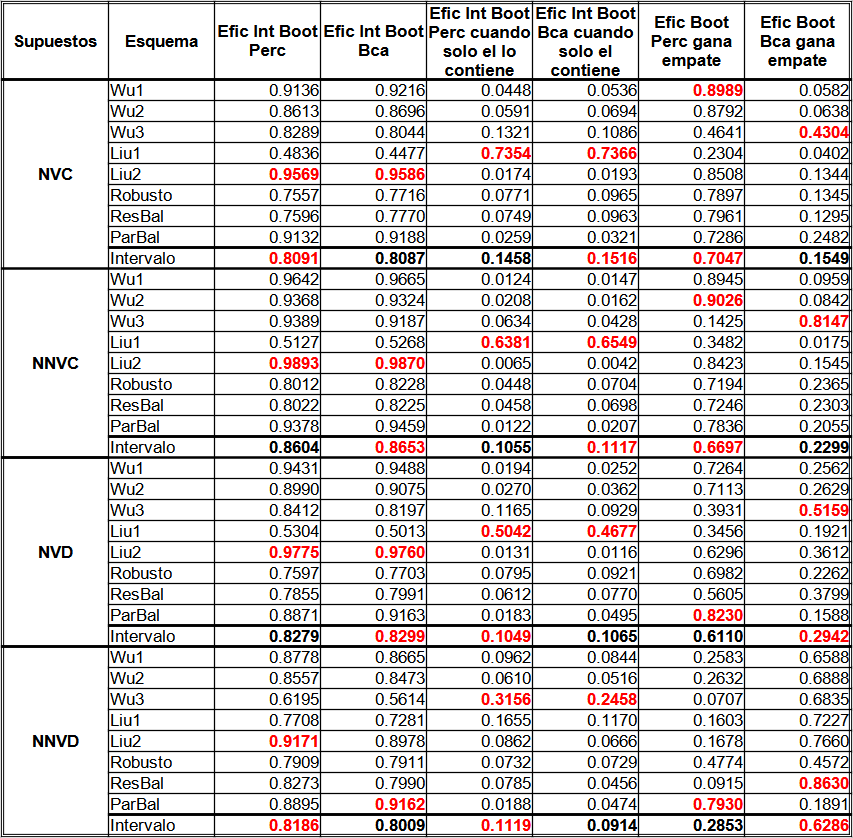
\includegraphics[width=0.80\linewidth]{img/EP_Prom_Supuestos.png} 
	\caption{Promedio de supuestos utilizados para el caso EP.} 
	\label{fig:EP_Supuestos}
\end{figure}
\FloatBarrier



%%%%%%%%%%%%%%%%%%%%%%%%%
%Empieza EI
\subsubsection{Eficiencia de los intervalos Bootstrap para el caso EI-NVC}
Con base en el promedio general (Figura 12) para: Eficiencia del ICB Percentil (Efic Int Boot Perc) y Eficiencia en ICB BCa (Efic Int Boot Bca) el mejor esquema resulto Liu2, 0.9627 y 0.9052 respectivamente;
 Eficiencia del ICB Percentil cuando solo el lo contiene a la $R^{2}$ y Eficiencia del ICB BCa cuando solo el contiene a la $R^{2}$ el mejor esquema resulto Liu1, 0.5864 y 0.5751 respectivamente; 
 la Eficiencia de ICB Percentil cuando gana en el empate a ICB BCa (Efic Boot Perc gana empate), el mejor esquema es Wu3 (0.3019) y la Eficiencia ICB BCa cuando gana el empate al ICB Percentil (Efic Boot Bca gana empate), el mejor esquema es Wu2 (0.8626).
\vspace{.5cm}


Sin considerar el tamaño de la muestra, para el caso EI-NVC los ICB mejores en promedio general (Figura 12) son: Eficiencia del ICB Percentil (Efic Int Boot Perc) con $0.8745$ ante la Eficiencia en ICB BCa (Efic Int Boot Bca); la Eficiencia del ICB Percentil cuando solo el contiene a la $R^{2}$ $(0.1413)$ y la Eficiencia de ICB BCa cuando gana en el empate al ICB Perc (Efic Boot Bca gana empate) con $0.7469$.

\begin{figure}[ht] 
	\centering 
	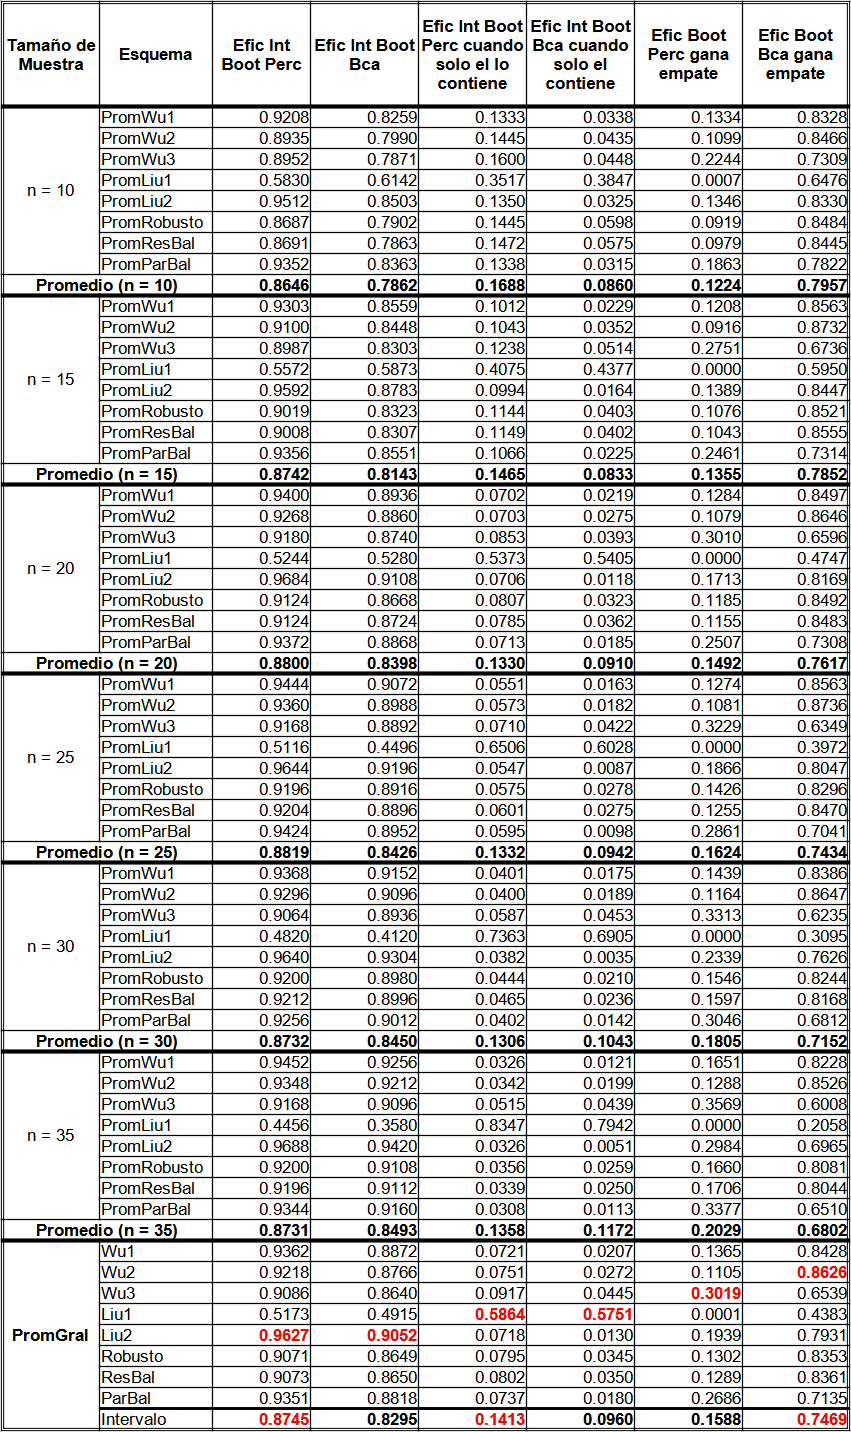
\includegraphics[width=0.55\linewidth]{img/EI_NVC_Efic_Boots.png} 
	\caption{Eficiencia promedio de los intervalos Bootstrap por tamaño de muestra y esquema de remuestreos para el caso EI-NVC.} 
	\label{fig:EI_NVC_Boots}
\end{figure}
\FloatBarrier


\subsubsection{Eficiencia de los esquemas para el caso EI-NVC}
Con base en el promedio de eficiencia por tamaño de muestra (Figura 12) y un nivel de confianza mayor o igual a 0.90: con tamaño de muestra 10 y 15 ningún esquema cumplió la condición, sin embargo con ambos el mejor esquema es Liu2, con 0.8227 y 0.8639 respectivamente; con los tamaños de muestra 20, 25, 30 el mejor fue el esquema Lui2 y con el tamaño de muestra 35 los mejores esquemas fueron Wu1, Wu2, Liu2 y Pareado Balanceado (ParBal).
\vspace{.5cm}

Sin considerar el tamaño de la muestra, para el caso EI-NVC el mejor promedio general (Figura 12) en eficiencia de esquema es Liu2 (0.8938).


\begin{figure}[ht] 
	\centering 
	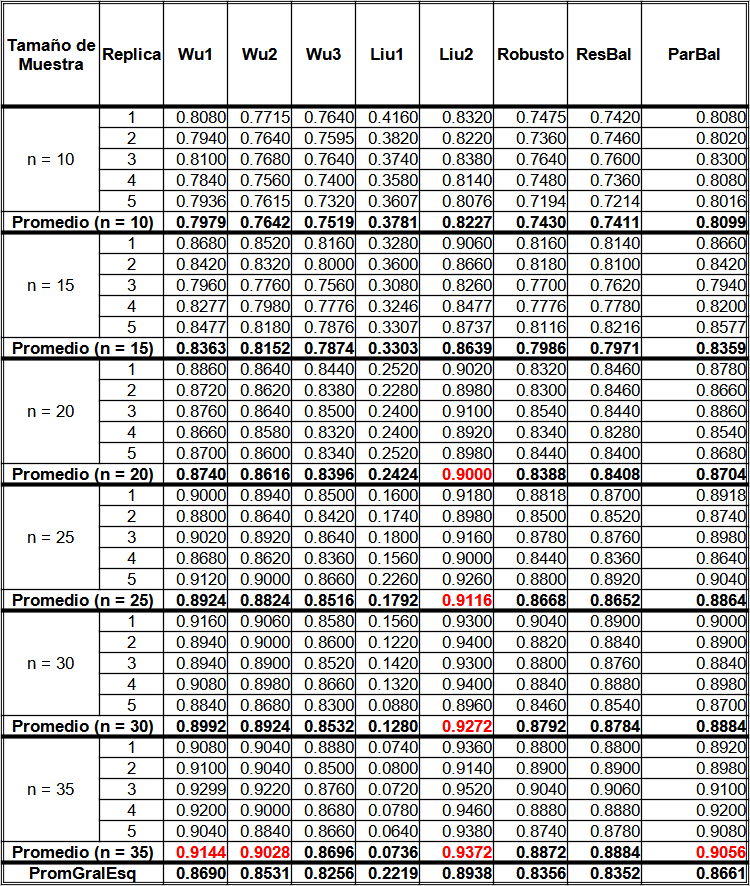
\includegraphics[width=0.70\linewidth]{img/EI_NVC_Efic_Esq.png} 
	\caption{Eficiencia promedio de los esquemas por tamaño de muestra y esquema de remuestreos para el caso EI-NVC.} 
	\label{fig:EI_NVC_Esq}
\end{figure}
\FloatBarrier


%%%%%%%%%%%%%%%%%%%%%%%%%%%%%%%%%%%%%%%

\subsubsection{Eficiencia de los intervalos Bootstrap para el caso EI-NNVC}
Con base en el promedio general (Figura 14) para: Eficiencia del ICB Percentil (Efic Int Boot Perc) y Eficiencia en ICB BCa (Efic Int Boot Bca) el mejor esquema resulto Liu2, 0.9603 y 0.9005 respectivamente;
 Eficiencia del ICB Percentil cuando solo el lo contiene a la $R^{2}$ y Eficiencia del ICB BCa cuando solo el contiene a la $R^{2}$ el mejor esquema resulto Liu1, 0.5224 y 0.5304 respectivamente; la Eficiencia de ICB Percentil cuando gana en el empate a ICB BCa (Efic Boot Perc gana empate), el mejor esquema es Wu3 (0.6169) y la Eficiencia ICB BCa cuando gana el empate al ICB Percentil (Efic Boot Bca gana empate), el mejor esquema es Pareado Balanceado (ParBal) con 0.7493.
\vspace{.5cm}

Sin considerar el tamaño de la muestra, para el caso EI-NNVC los ICB mejores en promedio general (Figura 14) son: Eficiencia del ICB Percentil (Efic Int Boot Perc) con $0.8833$ ante la Eficiencia en ICB BCa (Efic Int Boot Bca); la Eficiencia del ICB Percentil cuando solo el contiene a la $R^{2}$ $(0.1467)$ y la Eficiencia de ICB BCa cuando gana en el empate al ICB Perc (Efic Boot Bca gana empate) con $0.6252$.


\begin{figure}[ht] 
	\centering 
	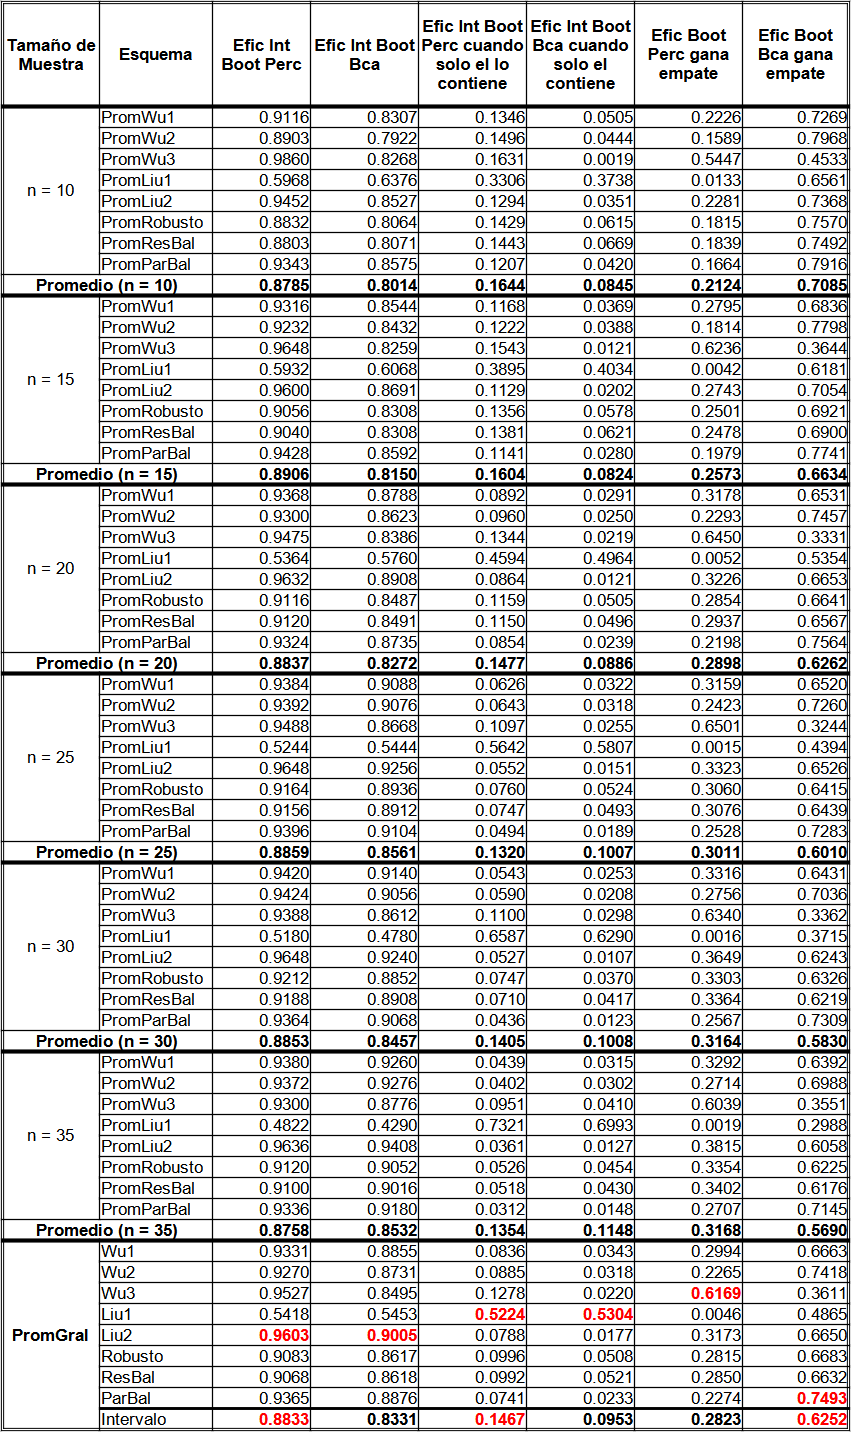
\includegraphics[width=0.55\linewidth]{img/EI_NNVC_Efic_Boots.png} 
	\caption{Eficiencia promedio de los intervalos Bootstrap por tamaño de muestra y esquema de remuestreos para el caso EI-NNVC.} 
	\label{fig:EI_NNVC_Boots}
\end{figure}
\FloatBarrier

\subsubsection{Eficiencia de los esquemas para el caso EI-NNVC}
Con base en el promedio de eficiencia por tamaño de muestra (Figura 15) y un nivel de confianza mayor o igual a 0.90: con los tamaños de muestra 10, 15 y 20 ningún esquema cumplió la condición, sin embargo, al no considerar el criterio anterior, el mejor esquema para: n=10 es Wu3 (0.8252) y Liu2 (0.8215), n=15 es Liu2 (0.8515) y Pareado Balanceado (ParBar) con 0.8352 y n=20 es Liu2 (0.8800) y Wu1 (0.8532). Con el tamaño de muestra 25 el mejor esquema es Liu2 (0.9116) seguido por ParBal (0.8932), con tamaño de muestra 30 el mejor esquema es Liu2 (0.9140) seguido por ParBal (0.8956) y con el tamaño de muestra 35 los mejores esquemas son Liu2 y ParBal, con 0.9288 y 0.904 respectivamente.
\vspace{.5cm}

Sin considerar el tamaño de la muestra, para el caso EI-NNVC los mejores promedios generales (Figura 15) en eficiencia de esquema son Liu2 (0.8848) y ParBal (0.8671).


\begin{figure}[ht] 
	\centering 
	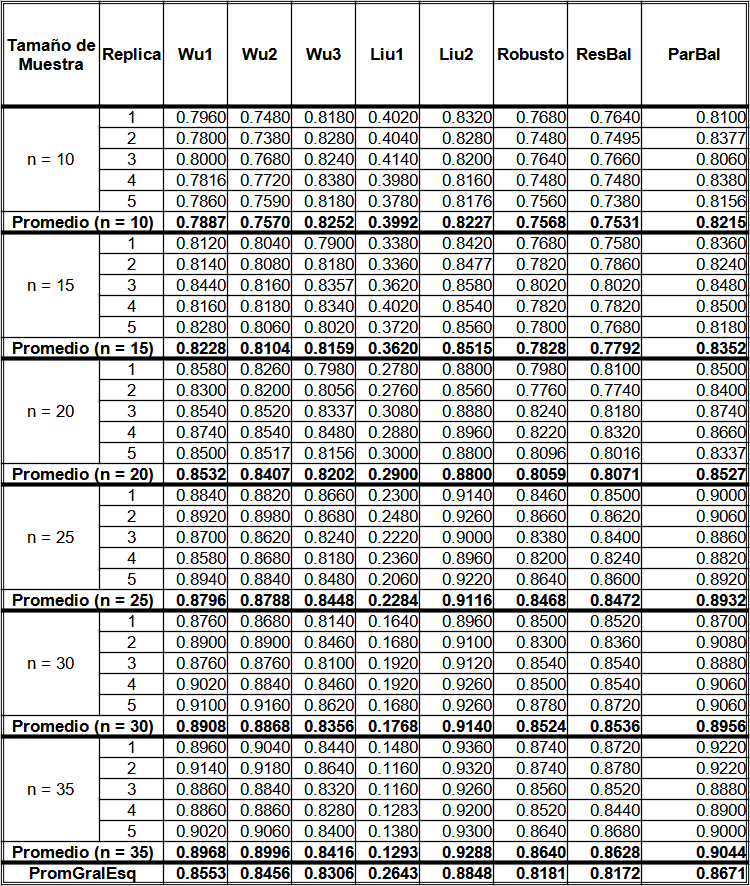
\includegraphics[width=0.70\linewidth]{img/EI_NNVC_Efic_Esq.png} 
	\caption{Eficiencia promedio de los esquemas por tamaño de muestra y esquema de remuestreos para el caso EI-NNVC.} 
	\label{fig:EI_NNVC_Esq}
\end{figure}
\FloatBarrier


%%%%%%%%%%%%%%%%%%%%%%%%%%%%%%%
\subsubsection{Eficiencia de los intervalos Bootstrap para el caso EI-NVD}
Con base en el promedio general (Figura 16) para: Eficiencia del ICB Percentil (Efic Int Boot Perc) el mejor esquema resulto Liu2 (0.9837), Eficiencia en ICB BCa (Efic Int Boot Bca) el mejor esquema resulto Pareado Balanceado(ParBal) con 0.8915; Eficiencia del ICB Percentil cuando solo el lo contiene a la $R^{2}$ y Eficiencia del ICB Bca cuando solo el contiene a la $R^{2}$ el mejor esquema resulto Liu1, 0.3799 y 0.3885 respectivamente; la Eficiencia de ICB Percentil cuando gana en el empate a ICB BCa (Efic Boot Perc gana empate), el mejor esquema es Residuales Balanceados(ResBal) con 0.3364 y la Eficiencia ICB BCa cuando gana el empate al ICB Percentil (Efic Boot Bca gana empate), el mejor esquema es Wu2 (0.7012).
\vspace{.5cm}


Sin considerar el tamaño de la muestra, para el caso EI-NVD los ICB mejores en promedio general (Figura 16) son: Eficiencia del ICB Percentil (Efic Int Boot Perc) con $0.9030$ ante la Eficiencia en ICB BCa (Efic Int Boot Bca); la Eficiencia del ICB Percentil cuando solo el contiene a la $R^{2}$ $(0.1402)$ y la Eficiencia de ICB BCa cuando gana en el empate al ICB Perc (Efic Boot Bca gana empate) con $0.6501$.


\begin{figure}[ht] 
	\centering 
	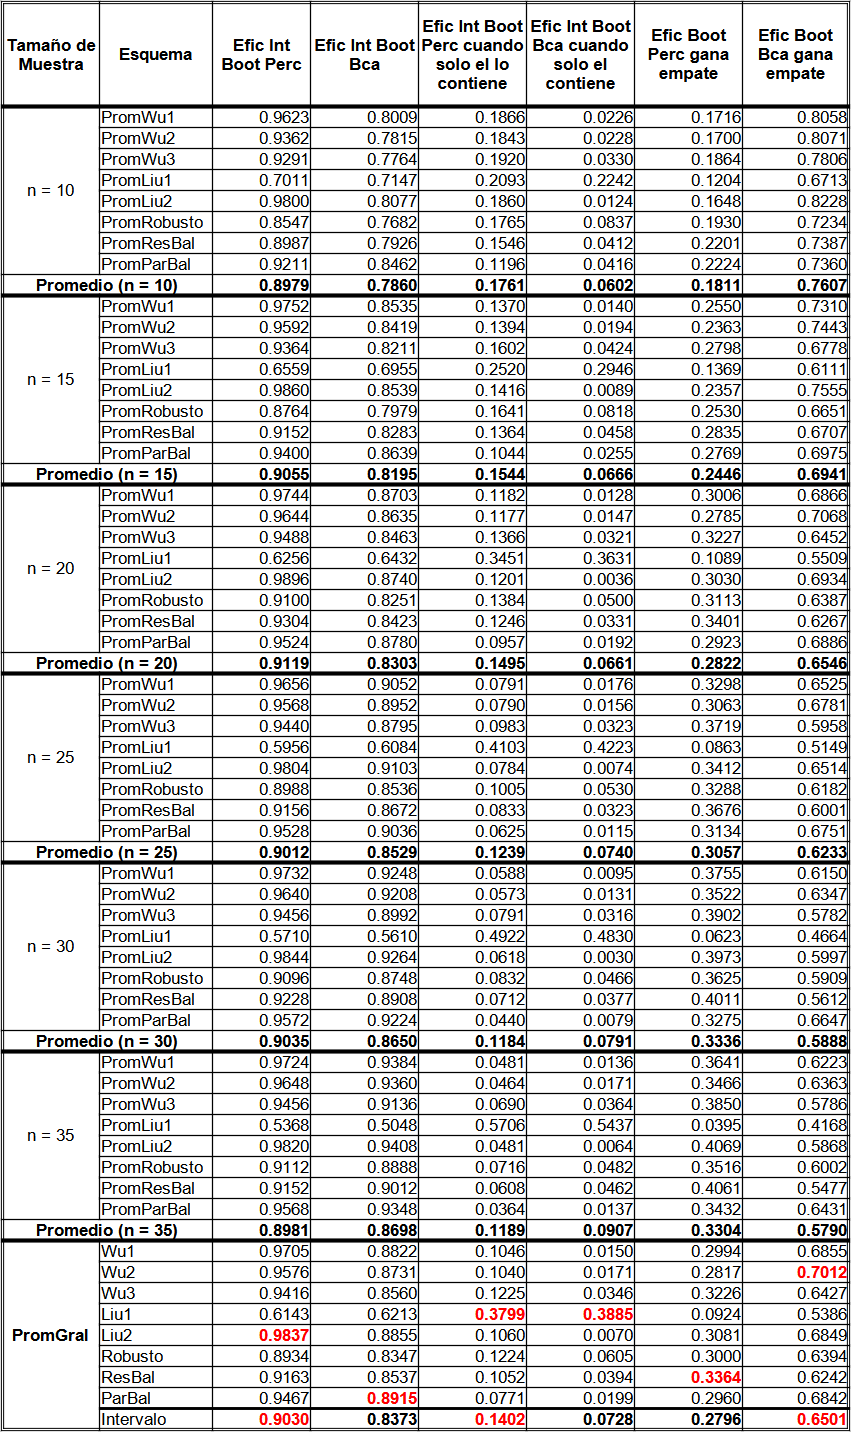
\includegraphics[width=0.55\linewidth]{img/EI_NVD_Efic_Boots.png} 
	\caption{Eficiencia promedio de los intervalos Bootstrap por tamaño de muestra y esquema de remuestreos para el caso EI-NVD.} 
	\label{fig:EI_NVD_Boots}
\end{figure}
\FloatBarrier



\subsubsection{Eficiencia de los esquemas para el caso EI-NVD}
Con base en el promedio de eficiencia por tamaño de muestra (Figura 17) y un nivel de confianza mayor o igual a 0.90: con tamaño de muestra 10, 15 y 20 ningún esquema cumplió la condición,
sin embargo, al no considerar el criterio anterior, el mejor esquema para: n=10 es Pareado Balanceado (ParBal) con 0.8110, Liu2 (0.7977), Wu1 (0.7829) y Wu2 (0.7637); n=15 es Liu2 (0.8463), ParBal (0.8419), Wu1 (0.8415) y Wu2 (0.8255), y n=20 Liu2 (0.8708), ParBal (0.8612), Wu1 (0.8591) y Wu2 (0.7637). Con el tamaño de muestra 25 el mejor esquema es Liu2 (0.9035) seguido por ParBal (0.8932), Wu1 (0.8892) y Wu2 (0.881); con tamaño de muestra 30 los mejores esquemas son Liu2 (0.9236),  Wu1 (0.9160), ParBal (0.9152) y Wu2 (0.9088), y con el tamaño de muestra 35 los mejores esquemas son Liu2 (0.9348),  Wu1 (0.9256), ParBal (0.922) y Wu2 (0.92).
\vspace{.5cm}

Sin considerar el tamaño de la muestra, para el caso EI-NVD el mejor promedio general (Figura 17) en eficiencia de esquema son Liu2 (0.8794), ParBal (0.8741), Wu1 (0.8690) y Wu2 (0.8583).


\begin{figure}[ht] 
	\centering 
	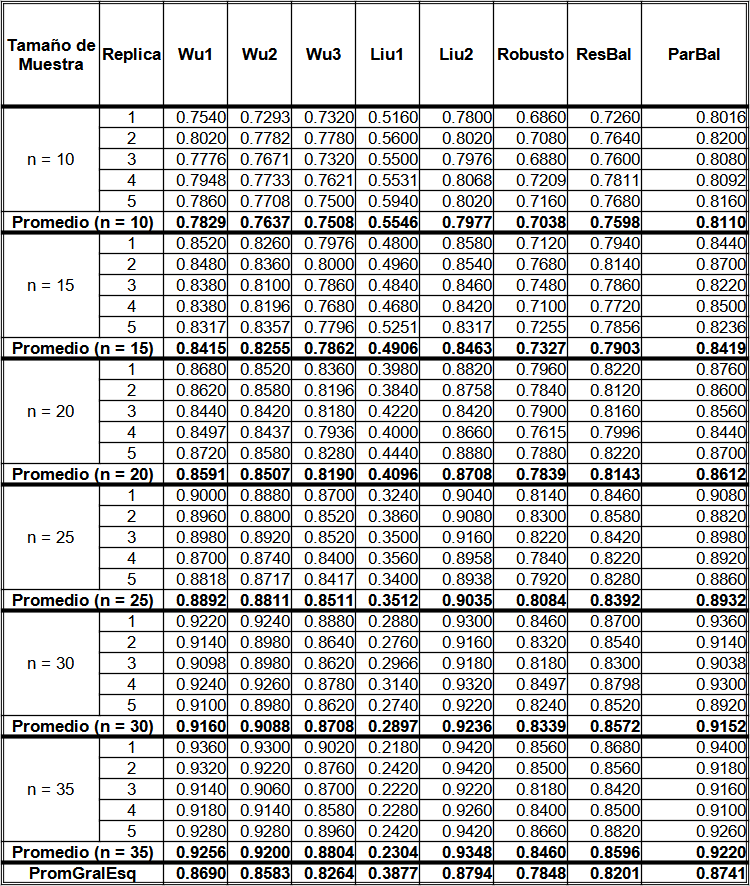
\includegraphics[width=0.70\linewidth]{img/EI_NVD_Efic_Esq.png} 
	\caption{Eficiencia promedio de los esquemas por tamaño de muestra y esquema de remuestreos para el caso EI-NVD.} 
	\label{fig:EI_NVD_Esq}
\end{figure}
\FloatBarrier


%%%%%%%%%%%%%%%%%%%%%%%%%%%%%%%%
\subsubsection{Eficiencia de los intervalos Bootstrap para el caso EI-NNVD}
Con base en el promedio general (Figura 18) para: Eficiencia del ICB Percentil (Efic Int Boot Perc) el mejor esquema resulto Liu2 (0.9554), Eficiencia en ICB BCa (Efic Int Boot Bca) el mejor esquema resulto Pareado Balanceado (ParBal) con 0.8882; Eficiencia del ICB Percentil cuando solo el lo contiene a la $R^{2}$ el mejor esquema resulto Wu3 (0.2807), Eficiencia del ICB BCa cuando solo el contiene a la $R^{2}$ el mejor esquema resulto Liu1 (0.1632); la Eficiencia de ICB Percentil cuando gana en el empate a ICB BCa (Efic Boot Perc gana empate), el mejor esquema es Residuales Balanceados(ResBal) con 0.5197 y la Eficiencia ICB BCa cuando gana el empate al ICB Percentil (Efic Boot Bca gana empate), el mejor esquema es ParBal (0.5074).
\vspace{.5cm}

Sin considerar el tamaño de la muestra, para el caso EI-NNVD los ICB mejores en promedio general (Figura 18) son: Eficiencia del ICB Percentil (Efic Int Boot Perc) con $0.9035$ ante la Eficiencia en ICB BCa (Efic Int Boot Bca); la Eficiencia del ICB Percentil cuando solo el contiene a la $R^{2}$ $(0.1940)$ y la Eficiencia de ICB BCa cuando gana en el empate al ICB Perc (Efic Boot Bca gana empate) con $0.5074$.

\begin{figure}[ht] 
	\centering 
	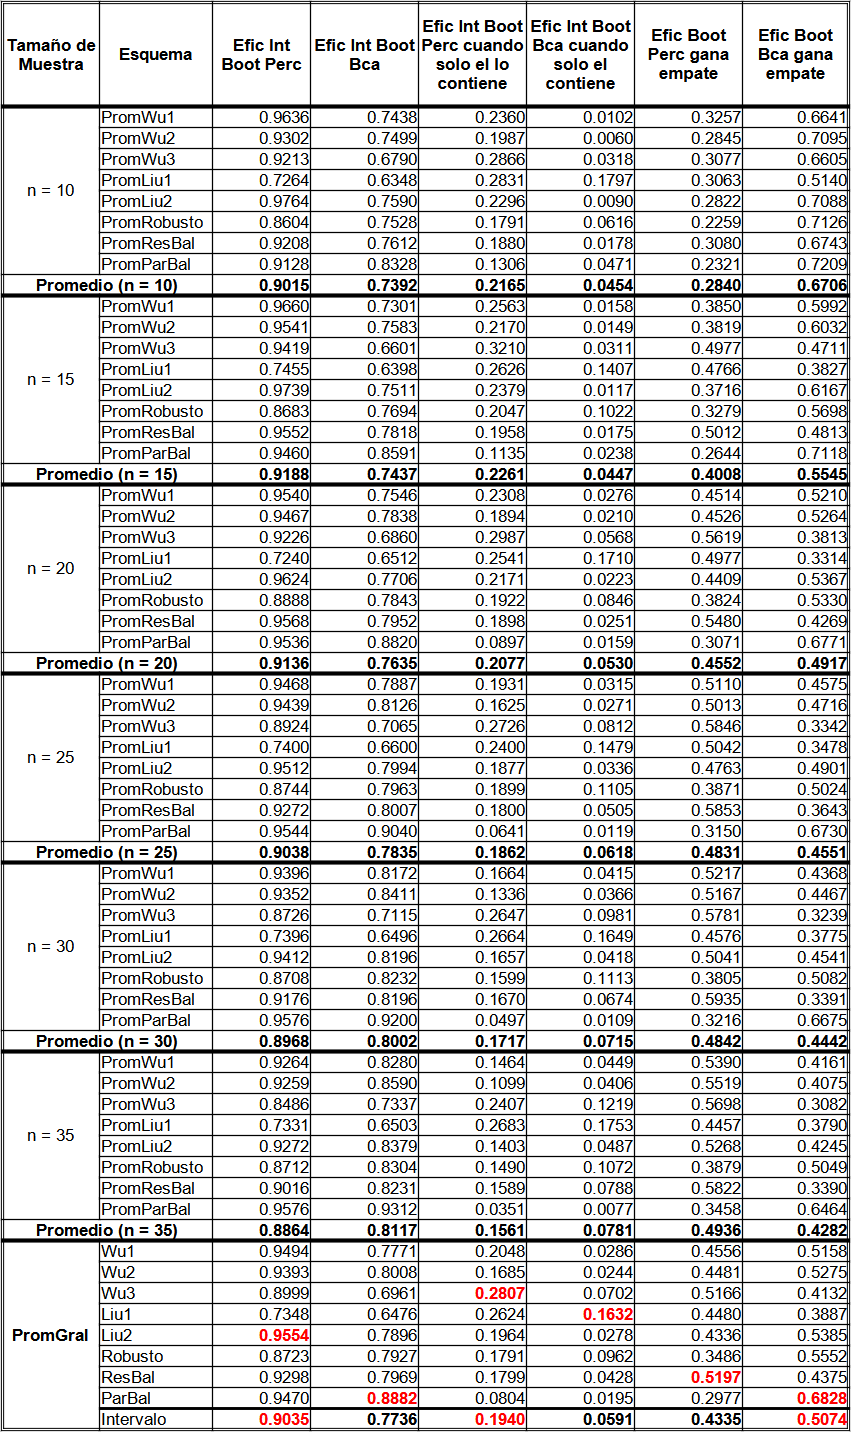
\includegraphics[width=0.55\linewidth]{img/EI_NNVD_Efic_Boots.png} 
	\caption{Eficiencia promedio de los intervalos Bootstrap por tamaño de muestra y esquema de remuestreos para el caso EI-NNVD.} 
	\label{fig:EI_NNVD_Boots}
\end{figure}
\FloatBarrier

\subsubsection{Eficiencia de los esquemas para el caso EI-NNVD}
Con base en el promedio de eficiencia por tamaño de muestra (Figura 18) y un nivel de confianza mayor o igual a 0.90: con tamaño de muestra 10, 15, 20 y 25 ningún esquema cumplió la condición, sin embargo, al no considerar el criterio anterior, el mejor esquema para: n=10 es Pareado Balanceado (ParBal) con 0.7936; n=15 es (ParBal) con 0.8387;  n=20 es ParBal (0.8680) y  n=25 es ParBal (0.8932). Con los tamaños de muestra 30 y 35 el mejor esquema es ParBal, 0.91 y 0.9240 respectivamente.
\vspace{.5cm}

Sin considerar el tamaño de la muestra, para el caso EI-NNVD el mejor promedio general (Figura 18) en eficiencia de esquema es ParBal (0.8713).


\begin{figure}[ht] 
	\centering 
	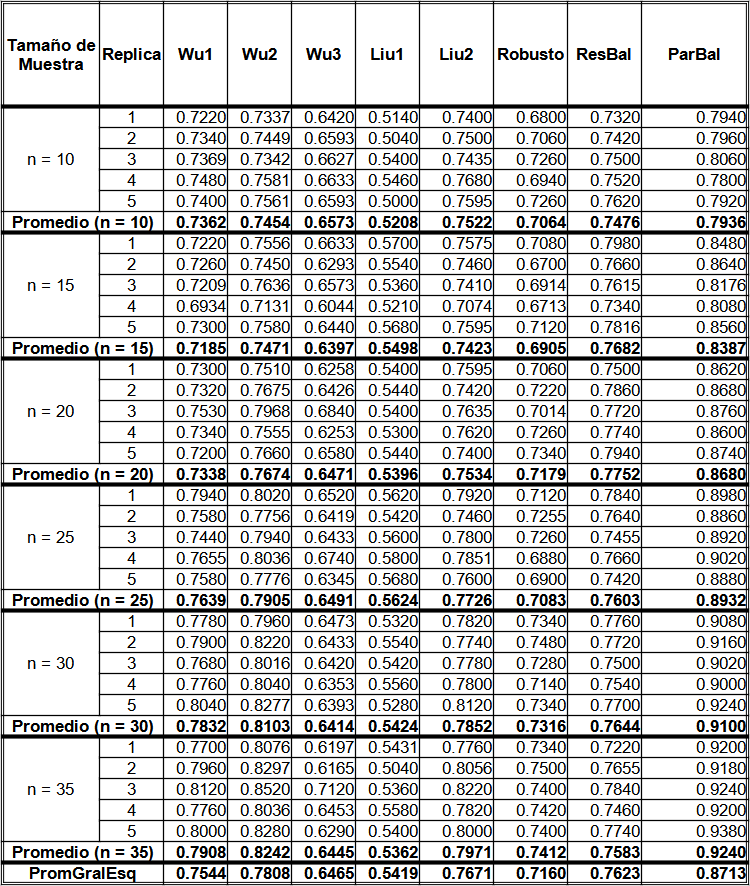
\includegraphics[width=0.70\linewidth]{img/EI_NNVD_Efic_Esq.png} 
	\caption{Eficiencia promedio de los esquemas por tamaño de muestra y esquema de remuestreos para el caso EI-NNVD.} 
	\label{fig:EI_NNVD_Esq}
\end{figure}
\FloatBarrier



%%%%%%%%%%%%%%%%%%%
\subsubsection{Promedio de supuestos para el caso EI}
Dados los modelos de tipo EI para los casos: Normalidad - Varianza Constante (NVC), No normalidad - Varianza Constante (NNVC), Normalidad - Varianza Distinta (NVD) y  No normalidad - Varianza Distinta (NNVD), con base en los promedios generales (Figura 20), se sugiere el uso de 
\begin{figure}[ht] 
	\centering 
	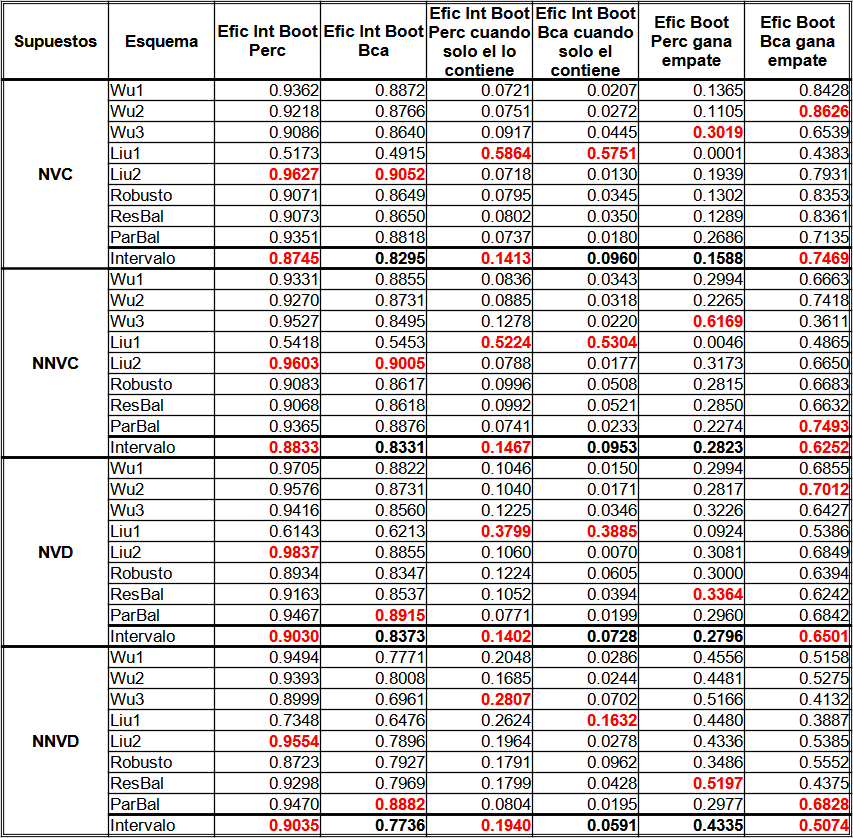
\includegraphics[width=0.80\linewidth]{img/EI_Prom_Supuestos.png} 
	\caption{Promedio de supuestos utilizados para el caso EI.} 
	\label{fig:EI_Supuestos}
\end{figure}







	\newpage
	\section{Conclusión}

En este trabajo se propuso un método para evaluar la precisión de un modelo con la técnica de regresión lineal; basado en ocho esquemas de remuestreo, dos tipos de modelo y seis tamaños de muestra; a través de dos intervalos de confianza Bootstrap para el coeficiente de determinación $R^2$, del modelo de regresión que resulta entre los valores reales y predichos del modelo a evaluar.\\

En la medición de la precisión, se consideraron cuatro escenarios posibles (NVC, NNVC, NVD y NNVD) para estimar la distribución del coeficiente de determinación $R^2$, mediante la implementación de los ocho esquemas de remuestreos: el Bootstrap simple, el Wild Bootstrap robusto con los tres esquemas propuestos por Wu (1986) y con los dos esquemas propuestos por Liu (1988), el Bootstrap de residuales balanceado y el Bootstrap pareado balanceado. Finalmente, por medio de los intervalos de confianza Bootstrap método percentil y Bca se estimó $R^2$ con $B=1,000$ remuestras para cada uno de los esquemas.\\

Se realizó un estudio de simulación para comparar las eficiencias de los intervalos de confianza para cada tipo de supuesto con respecto a los diferentes esquemas Bootstrap, tamaños de muestra y tipo de modelo; para ello se simularon mediante la propuesta de \textcite{febles-2014} y \textcite{zacarias-2023} , y evaluaron 60,000 modelos Exactos-Precisos (EP) y 60,000 modelos Exactos-Imprecisos (EI). Para cada modelo se identificó la $R^2$ de origen utilizada para su simulación.\\


Se consideraron tres criterios principales para determinar las eficiencias de los intervalos de confianza para cada esquema Bootstrap, el primer criterio determinó la eficiencia como el porcentaje de las veces en que el intervalo de confianza contiene a la $R^2$ de origen para los modelos EP simulados; y viceversa, para los modelos EI la eficiencia se determinó como el porcentaje de las veces en que el intervalo de confianza no contiene a la $R^2$ de origen. El segundo criterio determinó la eficiencia como el porcentaje de las veces en que ambos intervalos contienen de manera simultánea a la $R^2$ de origen para los modelos EP y cuando ambos no la contienen para los modelos EI; y el tercer criterio determinó la eficiencia como el porcentaje de las veces en que uno de los intervalos de confianza es más estrecho que el otro cuando ambos intervalos contienen simultáneamente la $R^2$ de origen para los modelos EP y de manera viceversa uno de los intervalos es más estrecho que el otro cuando ambos no la contienen simultáneamente para los modelos EI.\\
eficiencia
Se analizaron los resultados del estudio de simulación a través de un ANOVA factorial y se determinó con al menos un 95\% que para los supuestos NVC, NNVC o NVD se utilice el ICB Percentil con el esquema de remuestreo Liu2 sin importar el tamaño de muestra. Y se determinó con al menos el 88.8\% que para el supuesto NNVD se utilice el ICB BCa con el esquema de remuestreo pareado balanceado; con la limitación de que para modelos EI con tamaños de muestra “pequeño” $n=10, 15, 20,$ no se obtuvo un buen desempeño.\\


Con el propósito de que los resultados de este trabajo conformen una herramienta que permita evaluar la precisión de un modelo con la técnica de regresión lineal, se consideró como propuesta final: para los supuestos NVC, NNVC o NVD se utilice el ICB Percentil con el esquema de remuestreo Liu2 (NVC: residuales de regresión lineal simple, NNVC: residuales robustos sin ponderar y NVD: residuales robustos ponderados) y para el supuesto NNVD se utilice el ICB BCa con el esquema de remuestreo pareado balanceado. Esta herramienta se implementó en el lenguaje R.\\

En la aplicación de la propuesta final, para la ganancia diaria de peso en ovinos, el modelo resultó ser de tipo NVC y preciso, coincidiendo con \textcite{balam-2012}, cabe señalar que usó ICB BCa con residuales balanceados y en este trabajo se usó ICB Percentil con el esquema de remuestreo Liu2. Para el volumen por parcela, el modelo resultó de tipo NNVD y preciso, coincidiendo con \textcite{balam-2012}, tanto en la decisión como en el esquema e ICB que utilizó.\\


Como trabajo futuro, se podría desarrollar una librería en el lenguaje R que contenga la propuesta de este trabajo para la evaluación de la precisión, junto con la propuesta desarrollada por \textcite{zacarias-2023} para la evaluación de la exactitud y de esta manera tener una herramienta integral para la evaluación de un modelo con la técnica de regresión lineal. También esta propuesta se podría integrar al Sistema de Validación de Modelos \parencite{mazun-2014}, contribuyendo con un módulo más para la validación de un modelo. \\


Por ultimo, para otro trabajo futuro se propone evaluar otros ICB que requieren cómputos más exhaustivos pero utilizando la programación en paralelo.\\









	\newpage
	\printbibliography
	\newpage
	\section*{Anexo A. Tablas de Eficiencias de I.C. Bootstrap y Esquemas de los Modelo EI}


\textbf{EI-NVC}\\

\begin{figure}[ht] 
	\centering 
	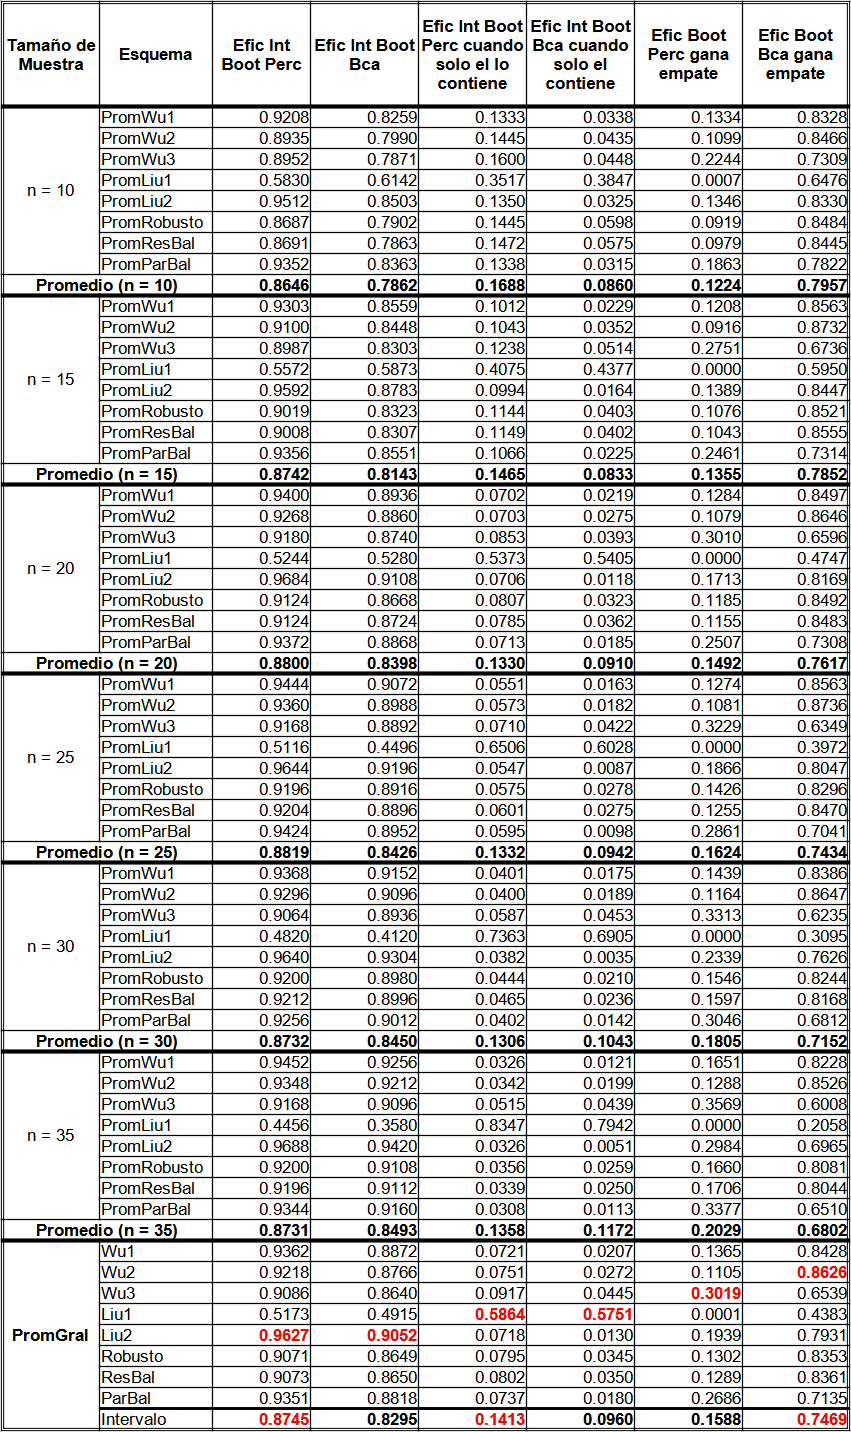
\includegraphics[width=0.55\linewidth]{img/EI_NVC_Efic_Boots.png} 
	\caption{Eficiencia promedio de los intervalos Bootstrap por tamaño de muestra y esquema de remuestreos para el caso EI-NVC.} 
	\label{fig:EficPromIntBootsTamMuestEsqRemuEI-NVC}
\end{figure}
\FloatBarrier


\begin{figure}[ht] 
	\centering 
	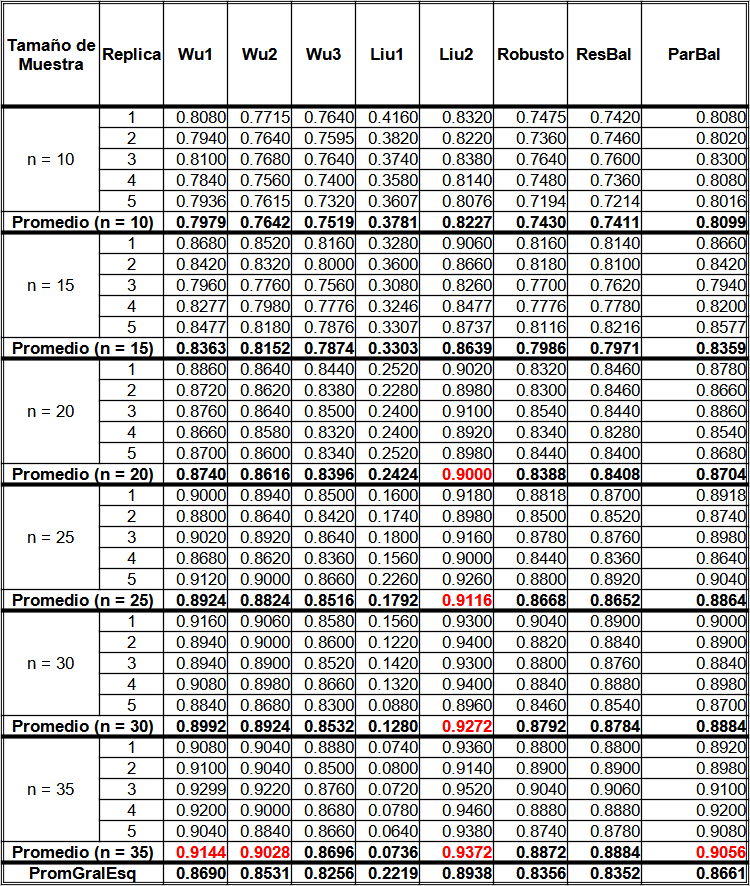
\includegraphics[width=0.70\linewidth]{img/EI_NVC_Efic_Esq.png} 
	\caption{Eficiencia promedio de los esquemas por tamaño de muestra y esquema de remuestreos para el caso EI-NVC.} 
	\label{fig:EficPromEsqTamMuesEsqRemuEI-NVC}
\end{figure}
\FloatBarrier


\textbf{EI-NNVC}\\

\begin{figure}[ht] 
	\centering 
	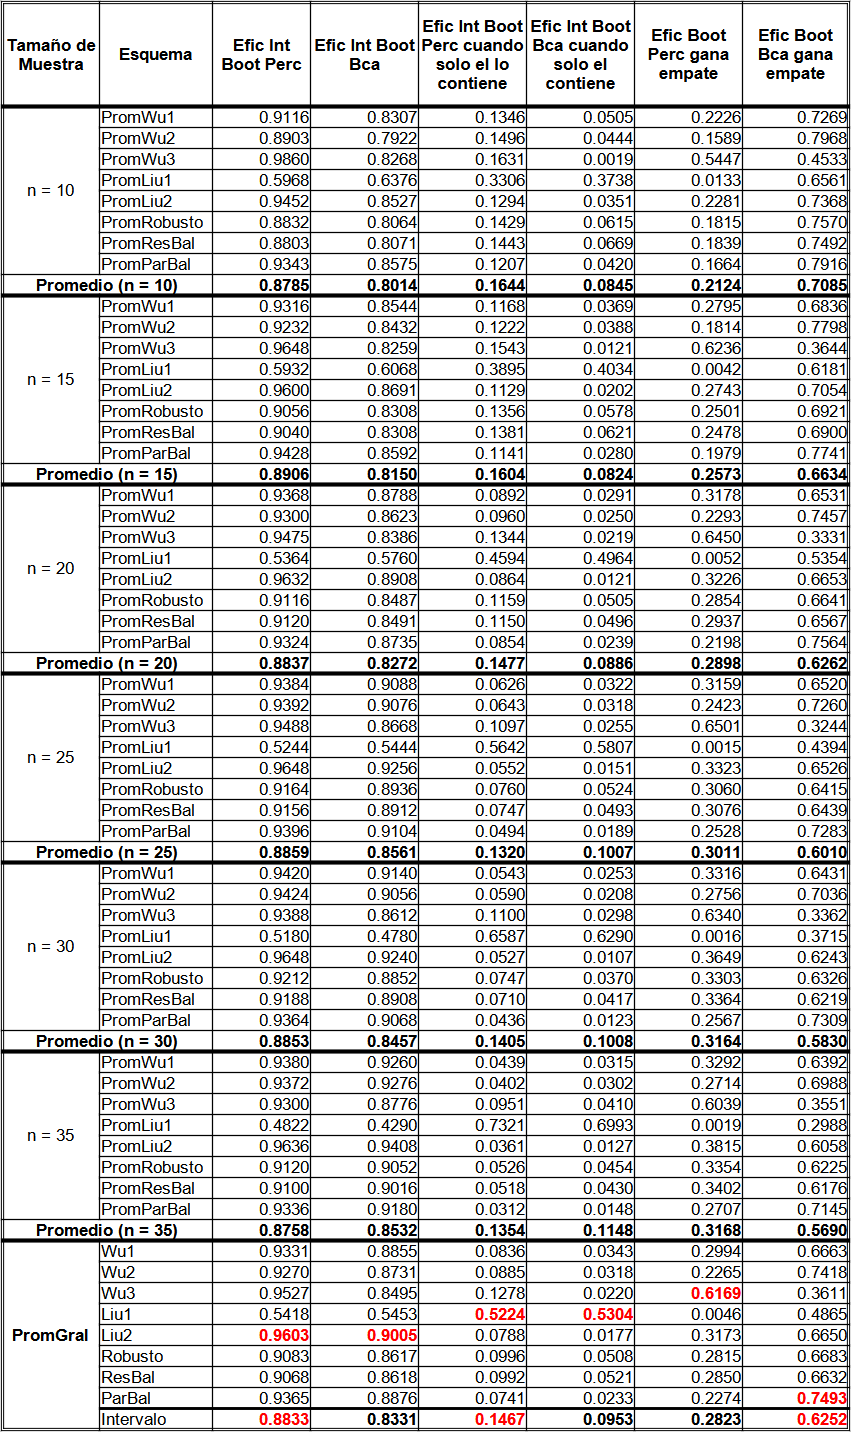
\includegraphics[width=0.55\linewidth]{img/EI_NNVC_Efic_Boots.png} 
	\caption{Eficiencia promedio de los intervalos Bootstrap por tamaño de muestra y esquema de remuestreos para el caso EI-NNVC.} 
	\label{fig:EficPromIntBootsTamMuestEsqRemuEI-NNVC}
\end{figure}
\FloatBarrier



\begin{figure}[ht] 
	\centering 
	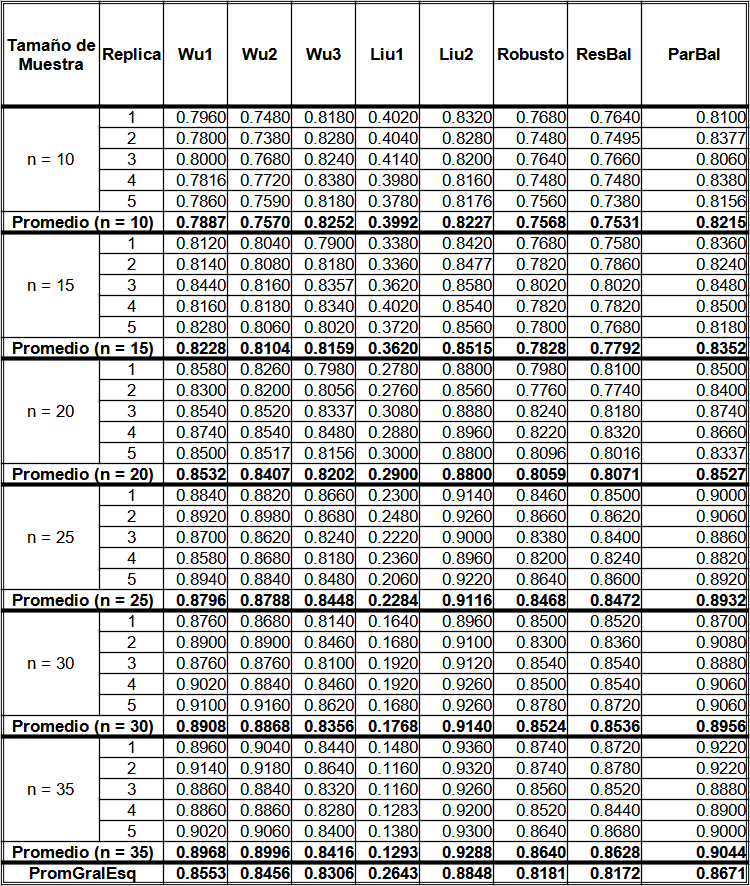
\includegraphics[width=0.70\linewidth]{img/EI_NNVC_Efic_Esq.png} 
	\caption{Eficiencia promedio de los esquemas por tamaño de muestra y esquema de remuestreos para el caso EI-NNVC.} 
	\label{fig:EficPromEsqTamMuesEsqRemuEI-NNVC}
\end{figure}
\FloatBarrier



\textbf{EI-NVD}\\

\begin{figure}[ht] 
	\centering 
	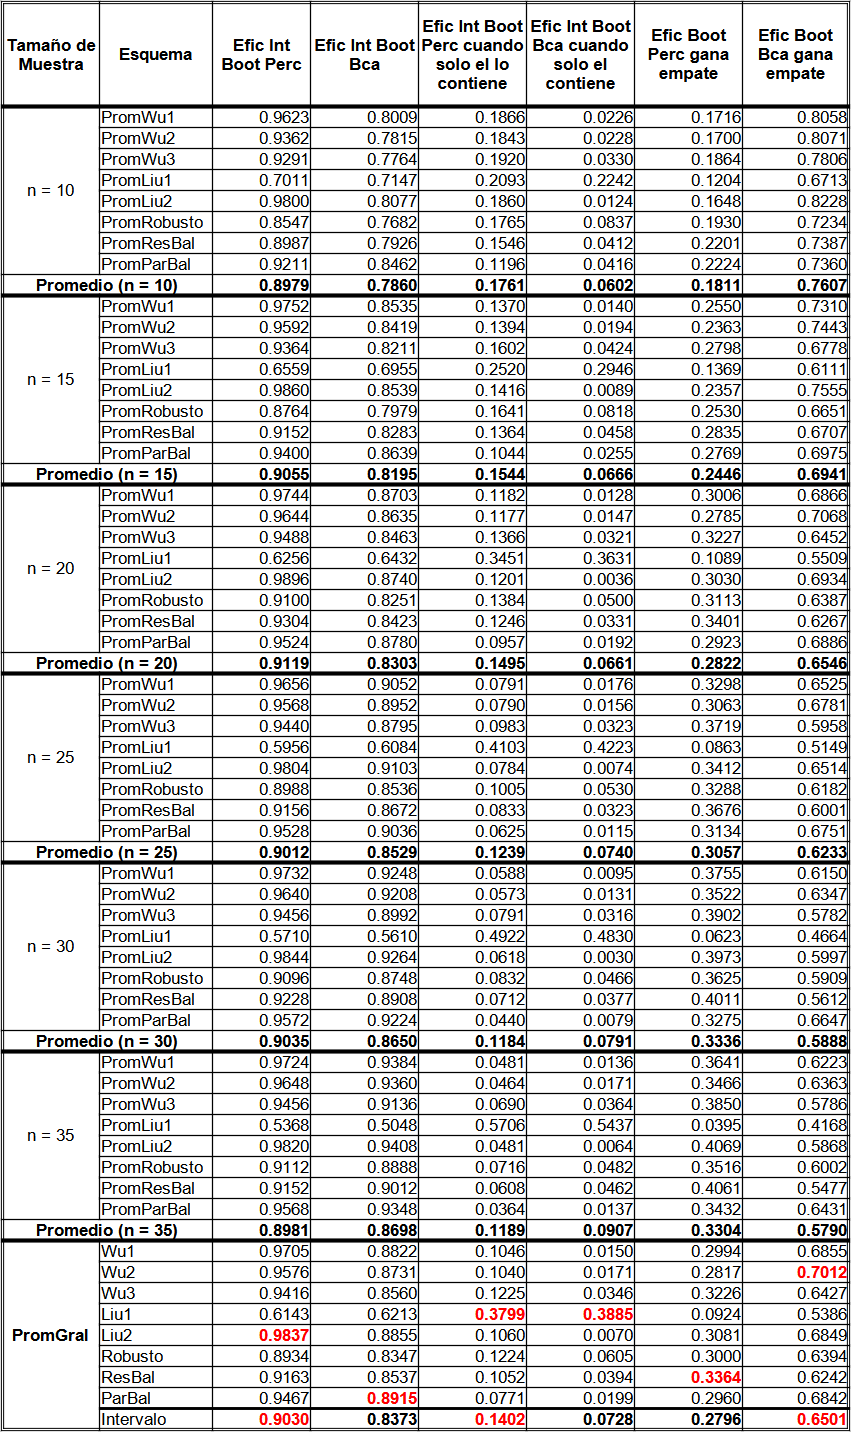
\includegraphics[width=0.55\linewidth]{img/EI_NVD_Efic_Boots.png} 
	\caption{Eficiencia promedio de los intervalos Bootstrap por tamaño de muestra y esquema de remuestreos para el caso EI-NVD.} 
	\label{fig:EficPromIntBootsTamMuestEsqRemuEI-NVD}
\end{figure}
\FloatBarrier


\begin{figure}[ht] 
	\centering 
	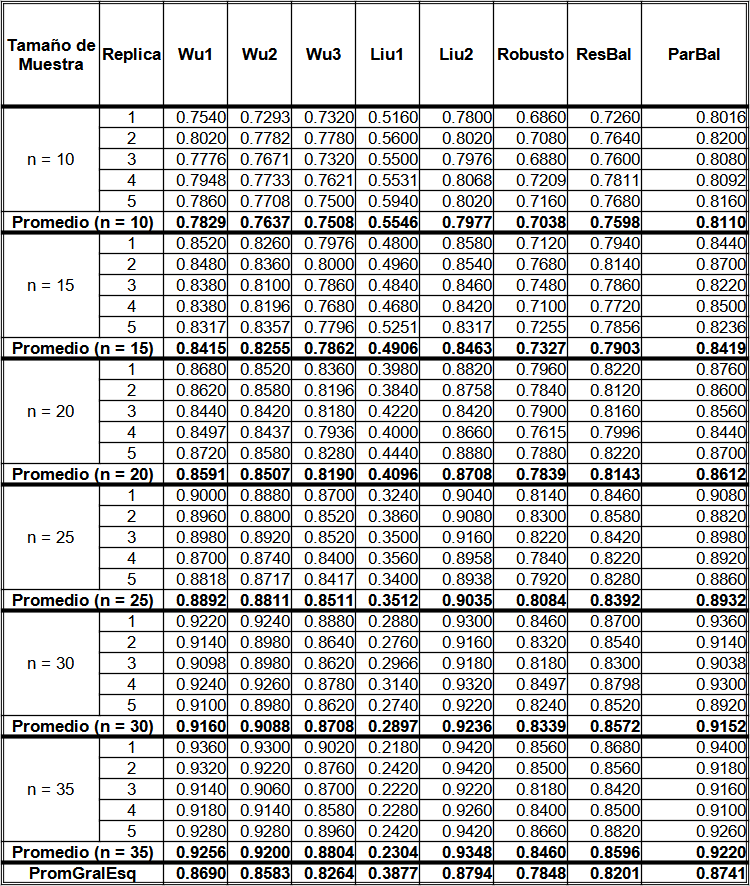
\includegraphics[width=0.70\linewidth]{img/EI_NVD_Efic_Esq.png} 
	\caption{Eficiencia promedio de los esquemas por tamaño de muestra y esquema de remuestreos para el caso EI-NVD.} 
	\label{fig:EficPromEsqTamMuesEsqRemuEI-NVD}
\end{figure}
\FloatBarrier




\textbf{EI-NNVD}\\

\begin{figure}[ht] 
	\centering 
	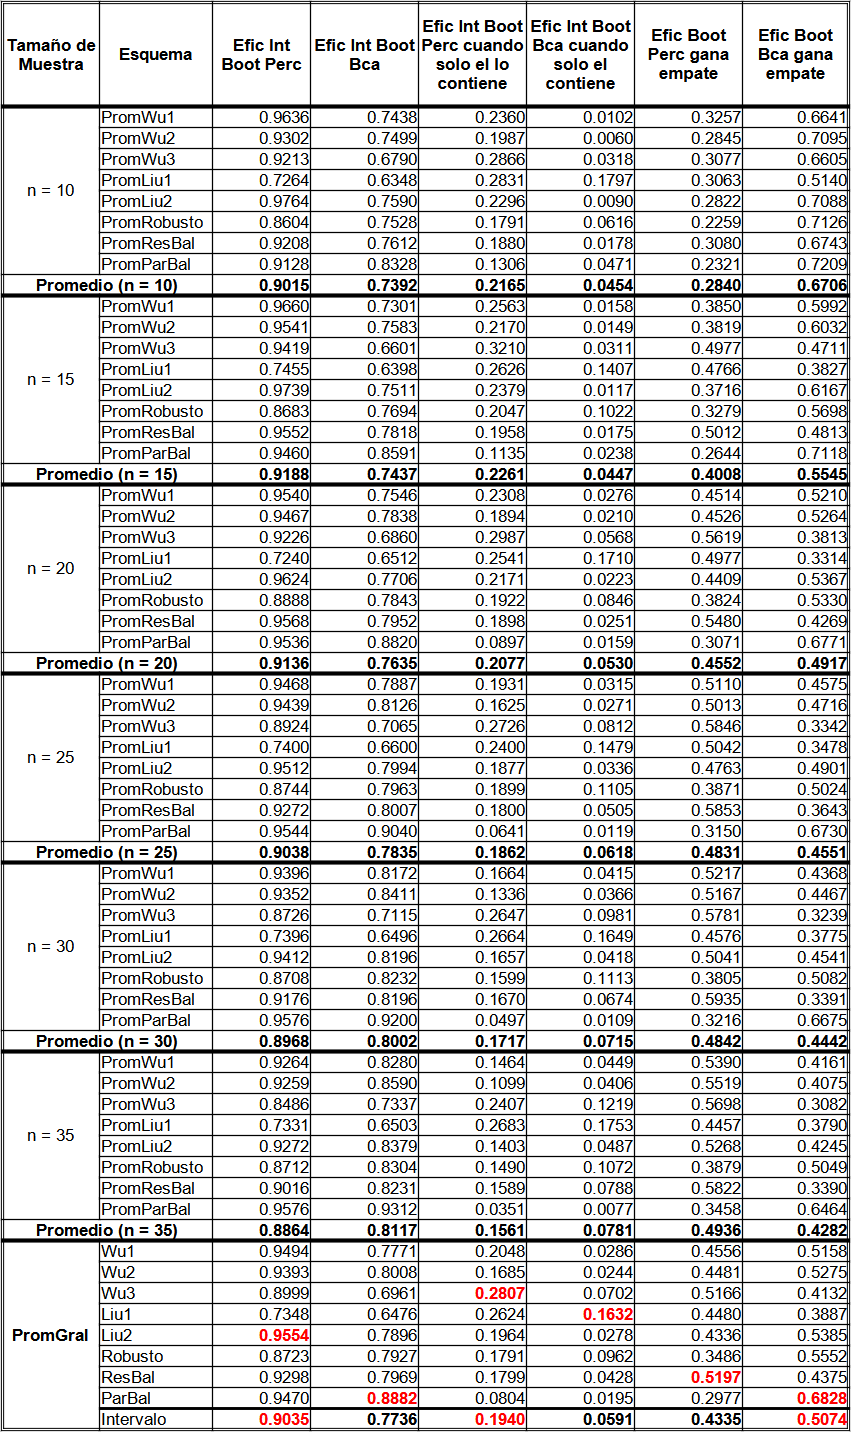
\includegraphics[width=0.55\linewidth]{img/EI_NNVD_Efic_Boots.png} 
	\caption{Eficiencia promedio de los intervalos Bootstrap por tamaño de muestra y esquema de remuestreos para el caso EI-NNVD.} 
	\label{fig:EficPromIntBootsTamMuestEsqRemuEI-NNVD}
\end{figure}
\FloatBarrier




\begin{figure}[ht] 
	\centering 
	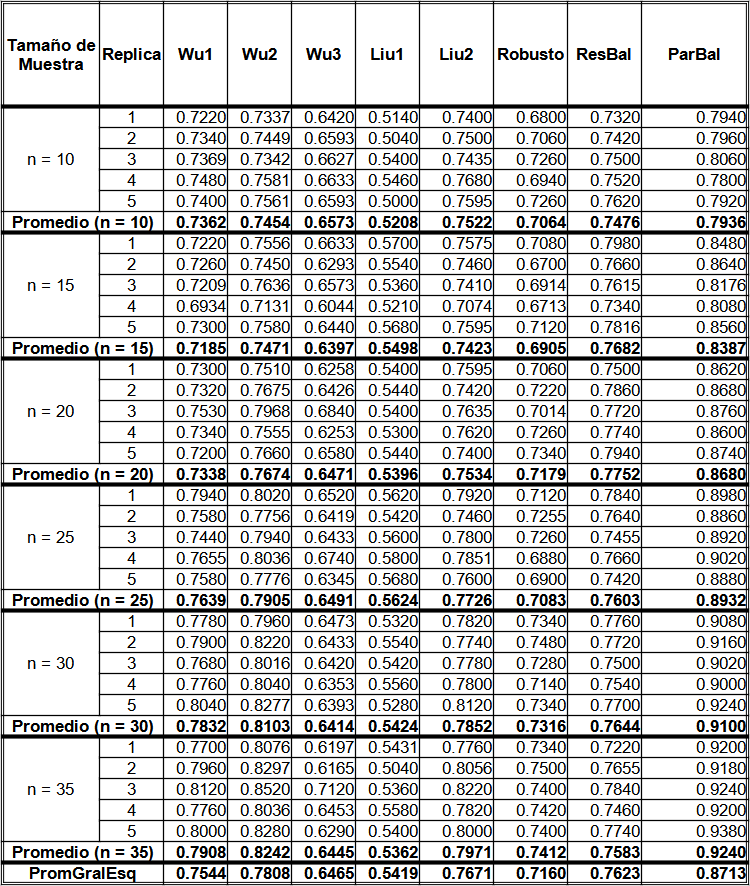
\includegraphics[width=0.70\linewidth]{img/EI_NNVD_Efic_Esq.png} 
	\caption{Eficiencia promedio de los esquemas por tamaño de muestra y esquema de remuestreos para el caso EI-NNVD.} 
	\label{fig:EficPromEsqTamMuesEsqRemuEI-NNVD}
\end{figure}
\FloatBarrier


\textbf{Para todos los supuestos para el caso EI}

\begin{figure}[ht] 
	\centering 
	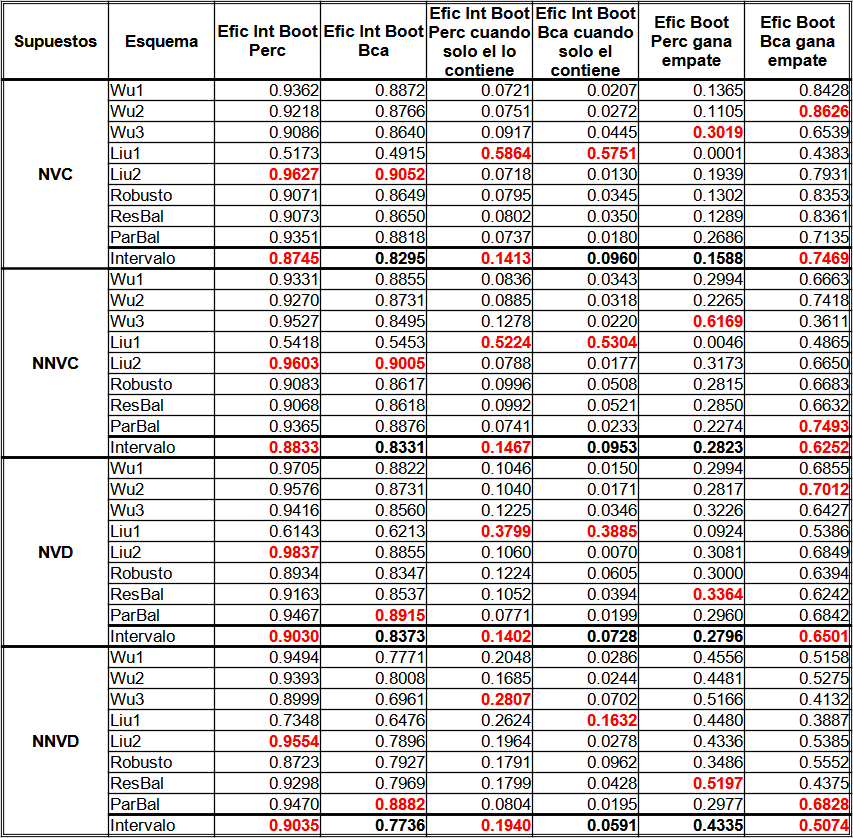
\includegraphics[width=0.80\linewidth]{img/EI_Prom_Supuestos.png} 
	\caption{Promedio de supuestos utilizados para el caso EI.} 
	\label{fig:PromSupuUtiliEI}
\end{figure}

\input{B_anexo.tex}
\newpage
\section*{Anexo C. Programas en R}
\addcontentsline{toc}{section}{Anexo C. Programas en R}

\subsection*{C1. Función CalcularR2Bootstrap}
\addcontentsline{toc}{subsection}{C1 Función CalcularR2Bootstrap}

En este anexo se muestra el script en R \parencite{R-2024}, el cual se utilizó para utilizar los esquemas Bootstrap dependiendo del caso del modelo.


\linespread{1}
\small
\begin{verbatim}
#Función de apoyo para obtener las muestras Bootstrap de R²
#Sea y <- los observador,
# z <- los estimados,
#yAjRob <- y ajustados 
#residuales <- residuales por regresion lineal,
#residualesRob <- residuales por regresion lineal robusta, 
#residualesRP <- residuales robustos ponderados,
#hii<- valor de aplacamiento del modelo con 
#regresion simple, n <- tamaño de la muestra de residuos, 
#B <- repeticiones Bootstrap,
#tipo <- sea el tipo de esquema Boostrap Robusto. 
#1<-Wu 1, 2<-Wu 2, 3<-Wu 3,
# 4<-Liu 1, 5<-Liu 2, 6<- Robusto/Simple
# 7<-residuales balanceados, 8<- pareado balanceado
CalcularR2Bootstrap <- function(y, z, yAjRob, residuales, 
					residualesRob, residualesRP, hii, n, B, tipo) {
	sqrt_hii <- sqrt(1 - hii)
	RsBoot <- numeric(B)
	
	if((tipo == 7) || (tipo ==8)){
		N     <- rep(1:n,B)
		NPerm <- sample(N)
	}
	
	for (i in 1:B) {
		
		residualBT <- switch(
		tipo,
		{
			tt <- rnorm(n)
			(tt * residualesRP) / sqrt_hii
		},
		{
			ai <- (residuales - mean(residuales)) / sd(residuales)
			tt <- sample(ai, replace = TRUE)
			(tt * residualesRP) / sqrt_hii
		},
		{
			mediana <- median(residualesRP)
			NMAD <- (1 / 0.6745) * median(abs(residualesRP - mediana))
			Rai <- (residualesRP - mediana) / NMAD
			tt <- sample(Rai, replace = TRUE)
			(tt * residualesRP) / sqrt_hii
		},
		{
			tt <- rgamma(n, 2, 4)
			(tt * residualesRP) / sqrt_hii
		},
		{
			media1 <- 0.5 * sqrt(17 / 6) + sqrt(1 / 6)
			media2 <- 0.5 * sqrt(17 / 6) - sqrt(1 / 6)
			H <- rnorm(n, media1, sqrt(0.5))
			D <- rnorm(n, media2, sqrt(0.5))
			tt <- H * D - media1 * media2
			(tt * residualesRP) / sqrt_hii
		},
		{
			sample(residualesRob, replace = TRUE)
		},
		{
			posI <- (i-1)*n+1
			posF <- i*n
			VPosi <- NPerm[posI:posF]
			residualesRP[VPosi]
		},
		{
			posI <- (i-1)*n+1
			posF <-i*n
			NPerm[posI:posF]
		},
		stop("Esquema no válido")
		)
		
		if(tipo != 8){
			yBoots <- yAjRob + residualBT
			modeloBoots <- lm(yBoots ~ z)
		}else{
			YP <- y[residualBT]
			ZP <- z[residualBT]
			modeloBoots <- lm(YP ~ ZP)
		}
		
		RsBoot[i] <- summary(modeloBoots)$r.squared
	}
	
	return(RsBoot)
}
\end{verbatim}


\newpage

\subsection*{C2. Función ContruirIntervBoot}
\addcontentsline{toc}{subsection}{C2. Función ContruirIntervBoot}

En este anexo se muestra el script en R \parencite{R-2024}, el cual se utilizó para la construcción de los ICB Percentil e ICB BCa.

\begin{verbatim}
#Función de apoyo para construir el intervalo de confianza 
#la muestra de R² Bootstraps del modelo
#Sea data <- los valores z e y del modelo,
# R2 <- la R² estimada del modelo, 
#muestrasR2Boot <- la muestra de R² Bootstrap,
# B <- repeticiones Bootstrap, nivConfianza<- nivel de confianza,
#tipo<- sea el tipo de intervalo de confiaza que desea construir,opciones:
#1<- percentil, 2<-BCa

ContruirIntervBoot <- function(data, R2, muestrasR2Boot, B, 
								nivConfianza, tipo){
	
	intervalo <- numeric(2) 
	alpha <- 1-nivConfianza
	z <- as.numeric(data[[1]])
	y <- as.numeric(data[[2]])
	vectorR2Bootstrap <- muestrasR2Boot
	
	intervalo <- switch(
	tipo,
	{
		puntosCriticos <- quantile(vectorR2Bootstrap, 
									c(alpha/2, 1 - alpha/2))
		as.vector(puntosCriticos)
	},
	{
		n <- length(z)
		z0 <- qnorm(mean(vectorR2Bootstrap < R2))
		suma0=0
		suma02=0
		suma03=0
		for(i in 1:n)
		{R2MI=summary(lm(y[-i]~z[-i]))$r.squared
			suma0=R2MI+suma0
		}
		R2PMI=suma0/n
		for(i in 1:n)
		{Dif0=R2PMI-summary(lm(y[-i]~z[-i]))$r.squared
			suma02=Dif0^2+suma02
			suma03=Dif0^3+suma03
		}
		a=suma03/(6*(suma02^1.5))
		
		z_alfa1 <- qnorm(alpha / 2)
		z_alfa2 <- qnorm(1 - alpha / 2)
		alfa1 <- pnorm(z0 + (z0 + z_alfa1) / (1 - a * (z0 + z_alfa1)))
		alfa2 <- pnorm(z0 + (z0 + z_alfa2) / (1 - a * (z0 + z_alfa2)))
		
		ICInfBootBCa <- quantile(muestrasR2Boot, alfa1)
		ICSupBootBCa <- quantile(muestrasR2Boot, alfa2)
		as.vector(c(ICInfBootBCa, ICSupBootBCa))
	},
	stop("Intervalo no válido")
	)
	
	return (intervalo)
}
\end{verbatim}

\newpage

\subsection*{C3. Función EvalPrecisionModel}
\addcontentsline{toc}{subsection}{C3. Función EvalPrecisionModel}

En este anexo se muestra el script en R \parencite{R-2024}, el cual se utilizó para evaluar la precisión de un modelo construyendo intervalos de confianza para cada esquema Bootstrap.\\

\begin{verbatim}
	
	#Función propuesta para evaluar la precisión de un modelo creando
	#intervalos de confianza con la tecnica de regresion lineal
	#con estimadores robustos y esquemas Booststrap
	#Sea data<- el modelo con las columnas z e y
	#caso <- 1 #Normalidad- homocedasticidad,
	#2 #Normalidad-heterocidasticidad,
	#3 #No normalidad-homocedasticidad y 
	#4 #No normalidad-heterocidastecidad 
	EvalPrecisionModel <- function (data, alpha, nivConfianza, caso){
		library("robustbase")
		library("readxl")
		z <- as.numeric(data[[1]])
		y <- as.numeric(data[[2]])
		n <- length(z)
		B <- 1000 #Remuestras bootstrap
		
		#Regresion lineal simple
		modeloLineal <- lm(y~z)
		residuales <- residuals(modeloLineal)
		R2 <- summary(modeloLineal)$r.squared
		hii <- hatvalues(modeloLineal)
		yAju <- fitted(modeloLineal)
		
		#Casos
		NVC <- 1 #Normalidad- homocedasticidad
		NVD <- 2 #Normalidad-heterocidasticidad
		NNVC <- 3 #No normalidad-homocedasticidad
		NNVD <- 4 #No normalidad-heterocidastecidad 
		numRemues <- 8 #Numero de tipos de remuestreos implementados
		rsBoot <- matrix(0,nrow = B, ncol = numRemues)
		
		#Uso de los estimadores dependendiendo el caso
		if(NVC == caso){
			#Minimos cuadrados
			residualesRob <- residuales
			yAjRob <- yAju
			residualesRP <- residuales
			
		}else{
			# Uso de estimador robusto MM  
			modeloLinealRob <- lmrob(y ~ z, method = "MM")
			residualesRob <- modeloLinealRob$residuals
			yAjRob <- modeloLinealRob$fitted.values
			
			#Segundo caso,no cumple normalidad, si varianza
			if(NNVC==caso){
				# Residuales robustos sin ponderacion
				residualesRP <- residualesRob
			}
			
			#Tercer caso, no hay homocedasticidad
			if((NNVD==caso) || (NVD==caso)){
				# Residuales robustos con ponderacion
				CMERob <- modeloLinealRob$scale**2
				#Llamar función para ponderar residuales
				residualesRP <- PodResidRobu (residualesRob,CMERob)
			}
		}
		
		#Procesamiento de los residuales en distintos esquemas
		for(i in 1:numRemues){
			BootR <- CalcularR2Bootstrap(y,z, yAjRob,residuales
			,residualesRob,residualesRP,hii,n,B,tipo=i)
			rsBoot[, i] <- BootR
		}
		resultadosInter <- vector("list", numRemues)
		
		#Cálculo de los intervalos para el R²
		for(i in 1:numRemues){
			muestrasR2Boot <- rsBoot[,i]
			perc <- ContruirIntervBoot(data,R2,muestrasR2Boot
			,B,nivConfianza=0.95,tipo=1)
			bca <- ContruirIntervBoot(data,R2,muestrasR2Boot,
			B,nivConfianza=0.95,tipo=2)
			resultadosInter[[i]] <- list(perc, bca)
		}
		
		return(resultadosInter)
	}
\end{verbatim}

\newpage
\subsection*{C4. Función ProcesarModels}
\addcontentsline{toc}{subsection}{C4. Función ProcesarModels}

En este anexo se muestra el script en R \parencite{R-2024}, el cual se utilizó para la evaluación de la precisión de los modelos.\\

\begin{verbatim}
# Función para procesar y capturar los resultados 
#sobre la precisión de las muestras con sus I.C.
# Dado archivos_encontrados <-  list(muestra,R2) 
#con rutas de archivos
# para el parametro caso, 1-NVC, 2-NVD, 3-NNVC, 4-NNVD
# para replicas sea el número de replicas
# con nivConfinza entre 0 - 1
# y sea para N el tamaño de las muestras
ProcesarModels <- function(archivos_encontrados, caso,
						 replicas, nivConfianza, N, MODELO, CASO) {
	library(openxlsx)
	library(readxl)
	archivo_muestra <- archivos_encontrados$muestra
	archivo_R2 <- archivos_encontrados$R2
	data_muestra <- read_excel(archivo_muestra, col_names = TRUE)
	data_R2 <- read_excel(archivo_R2, col_names = TRUE)
	
	block <- 1000
	cols_por_model <- 2
	limit_model <- 500 #modelos a procesar
	esquemas <- 8
	
	#Tablas de conteos
	nombre_cols <- c("Replica","Esquema", "NumMod", 
					"NumModEfic", "FrecEficIB1","FrecEficIB2",
	"FrecEficIB1Unico","FrecEficIB2Unico",
	"FrecEficIB1Emp2", "FrecEficIB2Emp2","NingunGanador")
	conteos_totales <- matrix(0, ncol = length(nombre_cols),
							 nrow = replicas * esquemas)
	colnames(conteos_totales) <- nombre_cols
	
	#Tabla de eficiencia
	nombre_cols_efi <- c("Replicas", "NumMod", "Esq1", 
						"Esq2", "Esq3", "Esq4", "Esq5",
						 "Esq6", "Esq7", "Esq8")
	conteo_efi <- matrix(ncol=length(nombre_cols_efi),
						nrow = replicas)
	colnames(conteo_efi) <- nombre_cols_efi
	
	nombre_archivo_conteos <- paste(MODELO, "__", 
								CASO, "__N", N, "__resultados_conteo__",
								 ".xlsx", sep = "")
	nombre_archivo_efi <- paste(MODELO, "__", CASO, "__N", 
							N,"__resultados_eficiencia__", ".xlsx", sep = "")
	
	#Creando libros de excel
	wb_conteos <- createWorkbook()
	addWorksheet(wb_conteos, "Conteos")
	wb_eficiencia <- createWorkbook()
	addWorksheet(wb_eficiencia, "Eficiencia")
	
	for (replica in 1:replicas) {
		print(paste("Replica #", replica))
		num_m <- 0 #num de modelos
		#Conteos por replica
		conteo_replica <- matrix(0, nrow = 8,
						 ncol = length(nombre_cols))
		replica_vector <- rep(replica, each = esquemas)
		esquema_vector <- rep(1:esquemas)#vector de 1-8
		numMode_vector <- rep(limit_model, each = esquemas)
		#Matriz de datos iniciales
		matriz_inicial <- cbind(replica_vector,
						 esquema_vector,numMode_vector)
		conteo_replica[, 1:3] <- matriz_inicial
		#Eficiencia por replica
		conteo_efi_replica <- numeric(length(nombre_cols_efi))
		conteo_efi_replica[1] <- replica
		#Indices de incio y fin de replica
		fila_inicio <- (replica - 1) * N + 1
		fila_fin <- replica * N
		replica_data <- data_muestra[fila_inicio:fila_fin, ]
		R2_replica <- as.numeric(data_R2[replica, ])
		
		#Procesamiento de fila replica
		for (i in seq(1, ncol(replica_data), by = block)) {
			block_end <- min(i + block - 1, ncol(replica_data))
			block_caso <- replica_data[, i:block_end]
			R2_block <- as.numeric(R2_replica[i:500])
			Rmod <- 0 #Indice de R² a procesar
			
			#Procesamiendo de modelos replica
			for (j in seq(1, ncol(block_caso), by = cols_por_model)) {
				model_end <- min(j + cols_por_model - 1, ncol(block_caso))
				modeloActual <- block_caso[, j:model_end]
				R2_modelo <- R2_block[Rmod + 1]
				Rmod <- Rmod + 1
				resultadosInter <- EvalPrecisionModel(modeloActual,
											 alpha, nivConfianza, caso)
											 #Funcion propuesta
				print(R2_modelo)
				print(resultadosInter)
				
				#Procesando resultados del modelo por esquema
				for (numEsquema in 1:length(resultadosInter)) {
					resultados_esquema <- resultadosInter[[numEsquema]]
					intervalos_ganadores <- list()
					modelo_esquema_eficaz <- TRUE # Bandera de modelo eficaz en esquema
					
					#Procesando intervalos por esquema
					for (numIntervalo in 1:length(resultados_esquema)) {
						intervalo <- resultados_esquema[[numIntervalo]]
						# Verifica si el intervalo es NaN
						if (any(is.na(intervalo)) || length(intervalo) != 2) {
							modelo_esquema_eficaz <- FALSE
							warning(paste("Intervalo inválido en esquema",
											 numEsquema, "intervalo", numIntervalo, 
							"Intervalo:", paste(intervalo, collapse = ","), 
							"con R2_modelo:", R2_modelo))
							break
						} else {
							# Intervalo es válido, revisar si contiene el R2
							if (!is.na(R2_modelo)) {
								R2_intervalo <- ifelse(R2_modelo
												 >= intervalo[1] & R2_modelo <= intervalo[2], 1, 0)
								if (R2_intervalo == 1) {
									intervalos_ganadores[[length(intervalos_ganadores) + 1]]
									 <- list(Intervalo = numIntervalo, 
									 	Longitud = intervalo[2] - intervalo[1])
								}
							}
						}
					}#Fin procesado intervalos por esquema
					
					# Si ambos intervalos fueron calculados correctamente
					if (modelo_esquema_eficaz) {
						conteo_replica[numEsquema, 4] <-
							 conteo_replica[numEsquema, 4] + 1 #Modelo eficiente
						
						
						# Lógica para ganador único o empate
						if (length(intervalos_ganadores) == 1) {
							if (intervalos_ganadores[[1]]$Intervalo == 1){
						conteo_replica[numEsquema, 5] <- conteo_replica[numEsquema, 5] + 1 
							#Eficiencia
						conteo_replica[numEsquema, 7] <- conteo_replica[numEsquema, 7] + 1
							 #Ganador
							}
							if (intervalos_ganadores[[1]]$Intervalo == 2){
							conteo_replica[numEsquema, 6] <- conteo_replica[numEsquema, 6] + 1 
							#Eficiencia
							conteo_replica[numEsquema, 8] <- conteo_replica[numEsquema, 8] + 1
							 #Ganador
							}
							
						} else if (length(intervalos_ganadores) == 2) {
							#Conteo ambas contuvieron a R²
							conteo_replica[numEsquema, 5]<-conteo_replica[numEsquema, 5]+1
							conteo_replica[numEsquema, 6]<-conteo_replica[numEsquema, 6]+1
							conteo_efi_replica[numEsquema+2]<-conteo_efi_replica[
																			numEsquema+ 2]+1 
							#Entro en los dos
							mejor_intervalo <- intervalos_ganadores[[which.min(
												sapply(intervalos_ganadores, function(x) x$Longitud))]]
							if (mejor_intervalo$Intervalo == 1) 
								conteo_replica[numEsquema, 9]<-conteo_replica[numEsquema, 9]+1
							if (mejor_intervalo$Intervalo == 2) 
								conteo_replica[numEsquema, 10]<-conteo_replica[numEsquema, 10]+1
						}else{
						conteo_replica[numEsquema, 11] <- conteo_replica[numEsquema, 11]+1 
						#Sin ganadores
						}
					}
					
				}#Fin por esquemas
				
				#Segumiento de modelos
				num_m <- num_m + 1
				if (num_m %% 50 == 0) {
					print(paste("Procesados", m, "modelos de replica",
								 replica, "/",replicas))
				}
				if (num_m == limit_model) {
					break
				}
				
			}#Fin de modelos replica
		}#Fin de replica
		
		#Guardar resultados obtenidos de replica
		fila_inicio <- (replica - 1) * esquemas + 1
		fila_fin <- replica * esquemas
		conteos_totales[fila_inicio:fila_fin, ] <- conteo_replica
		conteo_efi_replica[2] <- num_m
		conteo_efi[replica, ] <- conteo_efi_replica
		
		#Guardar resultados en xlsx
		writeData(wb_conteos, "Conteos", conteos_totales, 
				startCol = 1, startRow = 1, rowNames = FALSE)
		writeData(wb_eficiencia, "Eficiencia", conteo_efi,
				 startCol = 1, startRow = 1, rowNames = FALSE)
		saveWorkbook(wb_conteos, nombre_archivo_conteos, overwrite = TRUE)
		saveWorkbook(wb_eficiencia, nombre_archivo_efi, overwrite = TRUE)
		
	}#Fin de replicas
	
	cat("Fin de cálculos")
}
\end{verbatim}


\newpage
\subsection*{C5. Función SimMod}
\addcontentsline{toc}{subsection}{C5. Función SimMod}

En este anexo se muestra el script en R \parencite{R-2024}, el cual se utilizó para la simulación y el respaldo de todos los modelos.\\


\begin{verbatim}

##SIMULACION DE MODELOS##
#N=numero de modelos a simular
#n=tamano de la muestra
#r=numero de replicas por tamano
#TipoPres=tipo de presicion del modelo;
# 1:Preciso; 2:Impreciso
#TipoSupues=tipo de supuesto que cumple 
#el modelo de regresion; 1:NVC; 2:NVD; 3:NNVC; 4:NNVD
#Los modelos son exactos, b0=0 y b1=1

SimMod=function(N,n,r,TipoPres,TipoSupues)
{library(writexl)
	cat("\n\n Simulacion de modelos de tamano",n,"\n")
	A=matrix(nrow=n*r,ncol=2*N)#Matriz de modelos
	B=matrix(nrow=r,ncol=N)#Matriz de R2
	b0=0
	b1=1
	for(j in 1:r)
	{s=n*(j-1)+1
		m=j*n
		for(i in 1:N)
		{if(TipoPres==1){R2=round(runif(1,min=0.8,max=0.99),4)}
			if(TipoPres==2){R2=round(runif(1,min=0.1,max=0.3),4)}
			B[j,i]=R2
			muz=round(runif(1,5,100),0)
			li=2*(i-1)+1
			ls=2*i
			if(TipoSupues==1){A[s:m,li:ls]=ModNVC(n,b0,b1,R2,muz)}
			if(TipoSupues==2){A[s:m,li:ls]=ModNVD(n,b0,b1,R2,muz)}
			if(TipoSupues==3){A[s:m,li:ls]=ModNNVC(n,b0,b1,R2,muz)}
			if(TipoSupues==4){A[s:m,li:ls]=ModNNVD(n,b0,b1,R2,muz)}
			if(i%%100==0){cat("\nYa se simularon",
						i,"modelos de la replica",j,"\n")}
		}
		cat("\n Listo la replica",j,"\n")
	}
	
	#Guarda los modelos
	A=as.data.frame(A)
	if(TipoPres==1 && TipoSupues==1){nomarch="EPNVC"}
	if(TipoPres==1 && TipoSupues==2){nomarch="EPNVD"}
	if(TipoPres==1 && TipoSupues==3){nomarch="EPNNVC"}
	if(TipoPres==1 && TipoSupues==4){nomarch="EPNNVD"}
	if(TipoPres==2 && TipoSupues==1){nomarch="EINVC"}
	if(TipoPres==2 && TipoSupues==2){nomarch="EINVD"}
	if(TipoPres==2 && TipoSupues==3){nomarch="EINNVC"}
	if(TipoPres==2 && TipoSupues==4){nomarch="EINNVD"}
	nomarch=paste(nomarch,n)
	nomarch=paste(nomarch,".xlsx")
	write_xlsx(A,path=nomarch)
	
	#Guarda las R2
	B=as.data.frame(B)
	if(TipoPres==1 && TipoSupues==1){nomarch2="R2EPNVC"}
	if(TipoPres==1 && TipoSupues==2){nomarch2="R2EPNVD"}
	if(TipoPres==1 && TipoSupues==3){nomarch2="R2EPNNVC"}
	if(TipoPres==1 && TipoSupues==4){nomarch2="R2EPNNVD"}
	if(TipoPres==2 && TipoSupues==1){nomarch2="R2EINVC"}
	if(TipoPres==2 && TipoSupues==2){nomarch2="R2EINVD"}
	if(TipoPres==2 && TipoSupues==3){nomarch2="R2EINNVC"}
	if(TipoPres==2 && TipoSupues==4){nomarch2="R2EINNVD"}
	nomarch2=paste(nomarch2,n)
	nomarch2=paste(nomarch2,".xlsx")
	write_xlsx(B,path=nomarch2)
	cat("\n\n Fin de la simulacion de modelos de tamano n=",n,"\n\n")
}#Termina la funcion SimMod
\end{verbatim}


\newpage
\subsection*{C6. Ejecuciones de la Función SimMod}
\addcontentsline{toc}{subsection}{C6. Ejecuciones de la Función SimMod}

En este anexo se muestra el script en R \parencite{R-2024}, el cual se utilizó para ejecutar la simulación y el respaldo de todos los modelos.\\ 


\begin{verbatim}
#Genaración de las matrices de modelos y sus correspondiente R2 
#por cada tamano de muestra
#Modelos EPNVC por cada tamano de muestra
SimMod(N=500,n=10,r=5,TipoPres=1,TipoSupues=1)
SimMod(N=500,n=15,r=5,TipoPres=1,TipoSupues=1)
SimMod(N=500,n=20,r=5,TipoPres=1,TipoSupues=1)
SimMod(N=500,n=25,r=5,TipoPres=1,TipoSupues=1)
SimMod(N=500,n=30,r=5,TipoPres=1,TipoSupues=1)
SimMod(N=500,n=35,r=5,TipoPres=1,TipoSupues=1)

#Modelos EPNVD por cada tamano de muestra
SimMod(N=500,n=10,r=5,TipoPres=1,TipoSupues=2)
SimMod(N=500,n=15,r=5,TipoPres=1,TipoSupues=2)
SimMod(N=500,n=20,r=5,TipoPres=1,TipoSupues=2)
SimMod(N=500,n=25,r=5,TipoPres=1,TipoSupues=2)
SimMod(N=500,n=30,r=5,TipoPres=1,TipoSupues=2)
SimMod(N=500,n=35,r=5,TipoPres=1,TipoSupues=2)

#Modelos EPNNVC por cada tamano de muestra
SimMod(N=500,n=10,r=5,TipoPres=1,TipoSupues=3)
SimMod(N=500,n=15,r=5,TipoPres=1,TipoSupues=3)
SimMod(N=500,n=20,r=5,TipoPres=1,TipoSupues=3)
SimMod(N=500,n=25,r=5,TipoPres=1,TipoSupues=3)
SimMod(N=500,n=30,r=5,TipoPres=1,TipoSupues=3)
SimMod(N=500,n=35,r=5,TipoPres=1,TipoSupues=3)

#Modelos EPNNVD por cada tamano de muestra
SimMod(N=500,n=10,r=5,TipoPres=1,TipoSupues=4)
SimMod(N=500,n=15,r=5,TipoPres=1,TipoSupues=4)
SimMod(N=500,n=20,r=5,TipoPres=1,TipoSupues=4)
SimMod(N=500,n=25,r=5,TipoPres=1,TipoSupues=4)
SimMod(N=500,n=30,r=5,TipoPres=1,TipoSupues=4)
SimMod(N=500,n=35,r=5,TipoPres=1,TipoSupues=4)
#############################################
#Modelos IPNVC por cada tamano de muestra
SimMod(N=500,n=10,r=5,TipoPres=2,TipoSupues=1)
SimMod(N=500,n=15,r=5,TipoPres=2,TipoSupues=1)
SimMod(N=500,n=20,r=5,TipoPres=2,TipoSupues=1)
SimMod(N=500,n=25,r=5,TipoPres=2,TipoSupues=1)
SimMod(N=500,n=30,r=5,TipoPres=2,TipoSupues=1)
SimMod(N=500,n=35,r=5,TipoPres=2,TipoSupues=1)

#Modelos IPNVD por cada tamano de muestra
SimMod(N=500,n=10,r=5,TipoPres=2,TipoSupues=2)
SimMod(N=500,n=15,r=5,TipoPres=2,TipoSupues=2)
SimMod(N=500,n=20,r=5,TipoPres=2,TipoSupues=2)
SimMod(N=500,n=25,r=5,TipoPres=2,TipoSupues=2)
SimMod(N=500,n=30,r=5,TipoPres=2,TipoSupues=2)
SimMod(N=500,n=35,r=5,TipoPres=2,TipoSupues=2)

#Modelos IPNNVC por cada tamano de muestra
SimMod(N=500,n=10,r=5,TipoPres=2,TipoSupues=3)
SimMod(N=500,n=15,r=5,TipoPres=2,TipoSupues=3)
SimMod(N=500,n=20,r=5,TipoPres=2,TipoSupues=3)
SimMod(N=500,n=25,r=5,TipoPres=2,TipoSupues=3)
SimMod(N=500,n=30,r=5,TipoPres=2,TipoSupues=3)
SimMod(N=500,n=35,r=5,TipoPres=2,TipoSupues=3)

#Modelos IPNNVD por cada tamano de muestra
SimMod(N=500,n=10,r=5,TipoPres=2,TipoSupues=4)
SimMod(N=500,n=15,r=5,TipoPres=2,TipoSupues=4)
SimMod(N=500,n=20,r=5,TipoPres=2,TipoSupues=4)
SimMod(N=500,n=25,r=5,TipoPres=2,TipoSupues=4)
SimMod(N=500,n=30,r=5,TipoPres=2,TipoSupues=4)
SimMod(N=500,n=35,r=5,TipoPres=2,TipoSupues=4)
\end{verbatim}



\newpage
\subsection*{C7. Función EvaluaPrecICB}
\addcontentsline{toc}{subsection}{C7. Función EvaluaPrecICB}

En este anexo se muestra el script en R \parencite{R-2024}, el cual se utilizó para la propuesta final para evaluar la precisión de un modelo.


\begin{verbatim}

#Propuesta final
#Sean los parametros: data una matriz,
# con la columna 1 las "z" la columna 2 las "y" 
# y niConfinza un nivel de confinza entre 0-1
EvaluaPrecICB <- function(data, nivConfianza=0.95){
	library("nortest")
	library("lmtest")
	library("robustbase")
	
	z <<- as.numeric(data[[1]])
	y <<- as.numeric(data[[2]])
	n <<- length(z)
	B <<- 2500 #Remuestras bootstrap necesarias
	caso <<- 0
	IC_proces <<- 1 #Construir IC, metodo percentil como inicial
	alpha <<- 1-nivConfianza
	#Casos posibles
	NVC <- 1 #Normalidad- homocedasticidad
	NVD <- 2 #Normalidad-heterocidasticidad
	NNVC <- 3 #No normalidad-homocedasticidad
	NNVD <- 4 #No normalidad-heterocidastecidad 
	#Verificación de supuestos
	hay_normalidad <- FALSE
	varianza_constante <- FALSE
	media_cero <- FALSE
	hay_independencia <-FALSE
	conceptosClave <<- rep(0,4) #Banderas de apoyo en las 4 pruebas
	limite_precision <<-0.7
	
	#Regresion lineal simple
	modeloLineal <- lm(y~z)
	residuales <- residuals(modeloLineal)
	R2 <- summary(modeloLineal)$r.squared
	hii <- hatvalues(modeloLineal)
	yAju <- fitted(modeloLineal)
	
	# Función para imprimir texto con colores 
	print_colored <- function(text, text_color = 37, bg_color = NULL) {
		if (!is.null(bg_color)) {
			cat(sprintf("\033[%d;%dm%s\033[0m", text_color, bg_color, text))# Texto-fondo
		} else {
			cat(sprintf("\033[%dm%s\033[0m", text_color, text)) #Texto coloreado
		}
	}
	
	#Supuesto de normalidad
	{
		pValShap <- shapiro.test(residuales)$p.value  #Shapiro-Wilk
		ValCShap <- shapiro.test(residuales)$statistic
		pValLILLIE <- lillie.test(residuales)$p.value   #Lilliefort
		ValCLILLIE <- lillie.test(residuales)$statistic
		#Resultados
		pValor <- c(pValShap, pValLILLIE)
		ValorCal <- c(ValCShap, ValCLILLIE)
		Estadistica <- c("Shapiro-Wilk","Liliefort")
		tablaNormal <- data.frame(Estadistica,ValorCal,pValor)
		print_colored("\nPRUEBA DE NORMALIDAD\n", 37, 40)
		print(tablaNormal)
		
		pVal_Min <- min(pValor)
		hay_normalidad <-  pVal_Min > alpha
		
		if (hay_normalidad) {
			cat("\nConclusión: Se cumple el supuesto de normalidad
				 con Shapiro y Lilliefort al",alpha*100,"%.\n")
			conceptosClave[1] <- 1
		}else{
			cat("\nConclusión: No se cumple el supuesto 
				de normalidad con Shapiro y Lilliefort al",alpha*100,"%.\n")
			conceptosClave[1] <- 2
		}
	}#Fin prueba normalidad
	
	
	#Media cero
	{
		#Prueba
		pValor <-t.test(residuales)$p.value #test T-student
		ValorCal <- t.test(residuales)$statistic
		#Construccion de la tabla
		Estadistica = c("T-Student")
		tablaVar <- data.frame(Estadistica, ValorCal, pValor)
		print_colored("\nPRUEBA T-STUDENT PARA MEDIA CERO EN LOS RESIDUALES\n", 37, 40)
		print(tablaVar)
		media_cero <- alpha < pValor
		
		if(media_cero){
			cat("\nConclusión: Se cumple el supuesto de
				 media cero en los residuales al ",alpha*100,"%.\n")
			conceptosClave[3] <- 1
		}else{
			cat("\nConclusión: No se cumple el supuesto de 
				media cero en los residuales al",alpha*100,"%.\n")
			conceptosClave[3] <- 2
		}
	}#Fin de prueba de media cero
	
	
	
	#Prueba de varianzas
	{
		pValor <- 0
		prueba_var <- NULL
		aviso_varianza <- NULL
		ValorCal <- 0
		
		if(hay_normalidad){
			#Aplicar Breusch-Pagan Test
			pValor <- bptest(modeloLineal)$p.value
			ValorCal <- bptest(modeloLineal)$statistic
			conceptosClave[2] <- 1
			Estadistica <- c("Breush-Pagan")
		}else{
			#Aplicar White test
			pValor <- bptest(modeloLineal, varformula = ~ I(z^2))$p.value
			ValorCal <- bptest(modeloLineal, varformula = ~ I(z^2))$statistic
			conceptosClave[2] <- 2
			Estadistica <- c("White")
		}
		
		valorTestVa <-c(pValor)
		tablaVarianza <- data.frame(Estadistica,ValorCal, pValor)
		
		aviso_varianza <- switch(
		conceptosClave[2],
		{
			print_colored("\nPRUEBA DE IGUALDAD DE VARIANZAS CON BREUSH-PAGAN\n", 37, 40)
		},
		{
			print_colored("\nPRUEBA DE IGUALDAD DE VARIANZAS CON WHITE\n", 37, 40)
		},
		stop("Prueba invalida")
		)
		
		print(tablaVarianza)
		
		varianza_constante <- alpha < pValor
		
		if(varianza_constante){
			aviso_varianza <- switch(
			conceptosClave[2],
			{
				cat("\nConclusión: Se cumple el supuesto de varianza 
				constante con el estadístico de Breush-Pagan al",alpha*100,"%.\n")   
			},
			{
				cat("\nConclusión: Se cumple el supuesto de varianza 
				constante con el estadístico de White al",alpha*100,"%.\n")
			},
			stop("Prueba invalida")
			)
		}else{
			aviso_varianza <- switch(
			conceptosClave[2],
			{
				cat("\nConclusión: No se cumple el supuesto de varianza
				 constante con el estadístico de Breush-Pagan al",alpha*100,"%.\n")   
			},
			{
				cat("\nConclusión: No se cumple el supuesto de varianza 
				constante con el estadístico de White al",alpha*100,"%.\n")
			},
			stop("Prueba invalida")
			)
		}
	}#Fin prueba varianzas
	
	
	
	#Independencia
	{
		#Prueba
		pValor <- dwtest(modeloLineal)$p.value #Durbin-Watson test
		ValorCal <- dwtest(modeloLineal)$statistic
		Estadistica = c("Durbin-Watson test")
		tablaVar <- data.frame(Estadistica,ValorCal, pValor)
		print_colored("\nPRUEBA DE DURBIN-WATSON PARA INDEPENDENCIA\n", 37, 40)
		print(tablaVar)
		hay_independencia <- alpha < pValor
		
		if(hay_independencia){
			cat("\nConclusión: Se cumple el supuesto de
				 independencia con Durbin-Watson al",alpha*100,"%.\n")
			conceptosClave[4] <- 1
		}else{
			cat("\nConclusión: No se cumple el supuesto de
				 independencia con Durbin-Watson al",alpha*100,"%.\n")
			conceptosClave[4] <- 2
		}
	}#Fin de prueba independencia
	
	
	
	
	#Decision de caso que nos encontramos
	if(hay_normalidad && varianza_constante){
		caso <- NVC
		print_colored("\n ****** CASO: NORMALIDAD 
			- HOMOCEDASTICIDAD (NVC) ******\n", 37, 34)
	}else{
		# Uso de estimador robusto MM  
		modeloLinealRob <<- lmrob(y ~ z, method = "MM")
		
		if (hay_normalidad && !varianza_constante) {
			caso <- NVD
			print_colored("\n ****** CASO: NORMALIDAD 
				- HETEROCIDASTICIDAD (NVD) ******\n", 37, 34)
		}
		if(!hay_normalidad && varianza_constante){
			caso <- NNVC
			print_colored("\n ****** CASO: NO NORMALIDAD
				 - HOMOCEDASTICIDAD (NNVC) ******\n", 37, 34)
		}
		if(!hay_normalidad && !varianza_constante){
			caso <- NNVD
			print_colored("\n ****** CASO: NO NORMALIDAD
			 - HETEROCIDASTICIDAD (NNVD) ******\n", 37, 34)
			IC_proces <- 2
		}
	}
	
	RsBoot <<- numeric(B)#Remuestra de R^2
	#Comienza remuestreos Bootstrap para el coeficiente de determinación
	{
		if(caso != NNVD){
			
			residuales_utilizar <- switch(
			caso,
			{
				residuales #Usar minimos cuadrados -> NVC
			},
			{
				resTemp <- modeloLinealRob$residuals 
				CMERob <- modeloLinealRob$scale**2
				consPes <- 3
				x <- abs(resTemp)/sqrt(CMERob)
				w <- rep(1,n)
				xx <- which(x > consPes) 
				w[xx] <- (consPes / w[xx])
				w*resTemp #Usar residuales robustos ponderados MM-estimador->NVD
			},
			{
				modeloLinealRob$residuals #Usar residuales robustosMM-estimador ->NNVC
			},
			stop("Caso no valido para residuales")
			)
			
			yajus_usar <- if (caso == NVC ) yAju else modeloLinealRob$fitted.values
			
			#Efectuando Esquema Liu 2
			sqrt_hii <- sqrt(1 - hii)
			for (i in 1:B) {
				media1 <- 0.5 * sqrt(17 / 6) + sqrt(1 / 6)
				media2 <- 0.5 * sqrt(17 / 6) - sqrt(1 / 6)
				H <- rnorm(n, media1, sqrt(0.5))
				D <- rnorm(n, media2, sqrt(0.5))
				tt <- H * D - media1 * media2
				resBoot <- (tt * residuales_utilizar) / sqrt_hii
				yBoots <- yajus_usar + resBoot
				modeloBoots <- lm(yBoots ~ z)
				RsBoot[i] <- summary(modeloBoots)$r.squared
			}
		}else{#Caso NNVD
			N     <- rep(1:n,B)
			NPerm <- sample(N)
			for (i in 1:B) {
				posI <- (i-1)*n+1
				posF <- i*n
				pares_boots<- NPerm[posI:posF]
				YP <- y[pares_boots]
				ZP <- z[pares_boots]
				modeloBoots <- lm(YP ~ ZP)
				RsBoot[i] <- summary(modeloBoots)$r.squared
			}
		}
	}#Fin Bootstrap
	
	intervalo <- numeric(2)#Intervalo
	#Construir intervalo de confinza para R^2
	{
		intervalo <- switch(
		IC_proces,
		{
			puntosCriticos <- quantile(RsBoot, c(alpha/2, 1 - alpha/2))
			as.vector(puntosCriticos)
		},
		{
			z0 <- qnorm(mean(RsBoot < R2))
			suma0 <-0
			suma02<-0
			suma03<-0
			for(i in 1:n){
				R2MI<-summary(lm(y[-i]~z[-i]))$r.squared
				suma0<-R2MI+suma0
			}
			R2PMI<- suma0/n
			for(i in 1:n){
				Dif0<-R2PMI-summary(lm(y[-i]~z[-i]))$r.squared
				suma02<-Dif0^2+suma02
				suma03<-Dif0^3+suma03
			}
			a<-suma03/(6*(suma02^1.5))
			z_alfa1 <- qnorm(alpha / 2)
			z_alfa2 <- qnorm(1 - alpha / 2)
			alfa1 <- pnorm(z0 + (z0 + z_alfa1) / (1 - a * (z0 + z_alfa1)))
			alfa2 <- pnorm(z0 + (z0 + z_alfa2) / (1 - a * (z0 + z_alfa2)))
			
			ICInfBCa <- quantile(RsBoot, alfa1)
			ICSupBCa <- quantile(RsBoot, alfa2)
			as.vector(c(ICInfBCa, ICSupBCa))
		},
		stop("Intervalo no válido")
		)
	}
	
	#Resultado final
	{
		resultado <- switch(
		IC_proces,
		{
			print_colored("\nPRECISION (R2) CON EL 
			ICB PERCENTIL-ESQUEMA BOOTSTRAP LIU2   \n", 37, 40)
		},
		{
			print_colored("\nPRECISION (R2) CON EL
			 ICB BCa-ESQUEMA BOOTSTRAP PAREADO BALANCEADO \n", 37, 40)
		},
		stop("Prueba invalida")
		)
		
		Atributos <- c("R2","R2BootMedia","DesvEstR2Boots","LIR2","LSR2")
		Valores <- c(R2,mean(RsBoot),sd(RsBoot),intervalo[1],intervalo[2])
		tabla_IC <-data.frame(Atributos,Valores)
		print(tabla_IC)
		
		R2_preciso <- ifelse( (limite_precision>=intervalo[1]
			 & limite_precision <= intervalo[2]) ||
			 	 (intervalo[1] >= limite_precision) , 1, 0)
		
		conclusion <- switch(
		IC_proces,
		{
			if (R2_preciso == 1) {
				cat("\nConclusión: El modelo es preciso con
					 el ICB Percentil al ",nivConfianza*100,"%.\n")   
			}else{
				cat("\nConclusión: El modelo es impreciso con
					 el ICB Percentil al",nivConfianza*100,"%.\n")
			}
		},{
			if (R2_preciso == 1) {
				cat("\nConclusión: El modelo es preciso con
					 el ICB BCa al",nivConfianza*100,"%.\n")   
			}else{
				cat("\nConclusión: El modelo es impreciso con
				 el ICB BCa al",nivConfianza*100,"%.\n")
			}
		}
		)
		cat("\n Criterio: Si el ",limite_precision, " 
				está contenido en el ICB o es mayor
					 igual al limite inferior del ICB.\n")
	}#Fin de bloque final
	
}#Fin propuesta final	
\end{verbatim}









  
	
\end{document}